% Referências em
%% http://www.abntex.net.br/
% ------------------------------------------------------------------------
% ------------------------------------------------------------------------
% Template adaptado por Armando Leopoldo Keller - Unisinos
% ------------------------------------------------------------------------
% ------------------------------------------------------------------------



\documentclass[
	% -- opções da classe memoir --
	12pt,				% tamanho da fonte
	%openright,			% capítulos começam em pág ímpar (insere página vazia caso preciso)
	oneside,
	%twoside,			% para impressão em recto e verso. Oposto a oneside
	a4paper,			% tamanho do papel. 
	% -- opções da classe abntex2 --
	chapter=TITLE,		% títulos de capítulos convertidos em letras maiúsculas
	section=TITLE,		% títulos de seções convertidos em letras maiúsculas
	subsection=TITLE,	% títulos de subseções convertidos em letras maiúsculas
	%subsubsection=TITLE,% títulos de subsubseções convertidos em letras maiúsculas
	% -- opções do pacote babel --
	english,			% idioma adicional para hifenização
	french,				% idioma adicional para hifenização
	spanish,			% idioma adicional para hifenização
	brazil				% o último idioma é o principal do documento
	]{abntex2}

\usepackage{unisinos} % Necessário para customização para padrão da universidade

% Conserva as margens verticais sem arredondar a altura do bloco de texto.
\setulmarginsandblock{3cm}{2cm}{*}
\checkandfixthelayout[fixed]

% ---
% Pacotes básicos 
% ---
\usepackage[T1]{fontenc}		% Selecao de codigos de fonte.
\usepackage[utf8]{inputenc}		% Codificacao do documento (conversão automática dos acentos)
\usepackage{indentfirst}		% Indenta o primeiro parágrafo de cada seção.
\usepackage{color}				% Controle das cores
\usepackage{graphicx}			% Inclusão de gráficos
\usepackage{amsmath}			% Ambientes e comandos matemáticos (\text, align, etc.)
\usepackage{microtype} 			% para melhorias de justificação
\usepackage{seqsplit}			% permite quebra de sequências longas (identificadores)
% Permite quebra de linha dentro de identificadores em fonte monoespaçada
% (ex.: cmor2.0-0.9549), evitando que ultrapassem a margem direita.
\newcommand{\codigo}[1]{\texttt{\seqsplit{#1}}}
% ---
		
% ---
% Pacotes adicionais: Insira aqui os pacotes customizados para todo o documento
% ---
\usepackage{lipsum}				% para geração de dummy text
\usepackage{multirow}			% células com múltiplas linhas em tabelas
\usepackage{placeins}             % barreiras pontuais para preservar a sequência dos elementos
\usepackage{threeparttable}       % títulos e fontes na largura natural de tabelas e quadros
% ---

\usepackage{helvet}                         % Configuração da fonte padronizada no documento
\renewcommand{\familydefault}{\sfdefault}

% ---
% Pacotes de citações
% ---
%\usepackage[brazilian,hyperpageref]{backref}	 % Paginas com as citações na bibl
\usepackage[alf]{abntex2cite}	% Citações padrão ABNT

% ---
% Ajuste da colocação de floats: mantém figuras mais próximas de onde são
% referenciadas, aceitando maior área de float por página e mais floats por página.
% ---
\setcounter{topnumber}{3}
\setcounter{bottomnumber}{2}
\setcounter{totalnumber}{4}
\renewcommand{\topfraction}{0.9}
\renewcommand{\bottomfraction}{0.7}
\renewcommand{\textfraction}{0.1}
\renewcommand{\floatpagefraction}{0.75}
\setlength{\floatsep}{18pt plus 2pt minus 2pt}
\setlength{\textfloatsep}{12pt}
\setlength{\intextsep}{12pt}
% Evita uma linha isolada de parágrafo no início ou no final da página.
\clubpenalty=10000
\widowpenalty=10000
\displaywidowpenalty=10000

% Identificação em 12 pt e espaço simples. Fontes e notas usam os 10 pt
% de \ABNTEXfontereduzida, sem alterar a tipografia do texto principal.
\captionnamefont{\normalfont\normalsize}
\captiontitlefont{\normalfont\normalsize}
\captionstyle[\raggedright]{\raggedright}
\setlength{\abovecaptionskip}{0pt}
\setlength{\belowcaptionskip}{6pt}
\setfloatadjustment{figure}{\centering\SingleSpacing*\setlength{\parskip}{0pt}}
\setfloatadjustment{table}{\centering\SingleSpacing*\setlength{\parskip}{0pt}}
\newsavebox{\tccfigurebox} % conserva a largura efetiva das imagens limitadas pela altura
\newlength{\tccmaxdepth}
\newlength{\tccoutputdepth}
\NewCommandCopy{\tccfonte}{\fonte}
\renewcommand{\fonte}[2][\fontename]{%
  \begingroup
    \SingleSpacing*
    \setlength{\abovecaptionskip}{6pt}%
    \setlength{\belowcaptionskip}{0pt}%
    \tccfonte[#1]{#2}%
  \endgroup}

% --- late
% CONFIGURAÇÕES DE PACOTES
% ---

% ---
% Configurações do pacote backref (desativado)
% \renewcommand{\backrefpagesname}{Citado na(s) página(s):~}
% \renewcommand{\backref}{}
% \renewcommand*{\backrefalt}[4]{
% 	\ifcase #1 %
% 		Nenhuma citação no texto.%
% 	\or
% 		Citado na página #2.%
% 	\else
% 		Citado #1 vezes nas páginas #2.%
% 	\fi}%
% ---

% ---
% Informações de dados para CAPA e FOLHA DE ROSTO
% ---
\titulo{Análise de Padrões de Escoamento Bifásico em Microcanais Utilizando Processamento Digital de Sinais}
\autor{Luís Felipe Lewandoski Borsoi}
\local{São Leopoldo}
\data{2026}
\orientador{Prof. Jean Schmith}
%\coorientador{Equipe \abnTeX}
\instituicao{%
  UNIVERSIDADE DO VALE DO RIO DOS SINOS -- UNISINOS
  \par
  UNIDADE ACADÊMICA DE GRADUAÇÃO
  \par
  CURSO DE ENGENHARIA DA COMPUTAÇÃO}
\tipotrabalho{Monografia (graduação)}
% O preambulo deve conter o tipo do trabalho, o objetivo,
% o nome da instituição e a área de concentração
\preambulo{Trabalho de Conclusão de curso apresentado como requisito parcial para obtenção do título de Bacharel em Engenharia da Computação, pelo curso de Engenharia da Computação da Universidade do Vale do Rio dos Sinos (UNISINOS).}
% ---


% ---
% Configurações de aparência do PDF final

% alterando o aspecto da cor azul
%\definecolor{blue}{RGB}{41,5,195}
\definecolor{blue}{RGB}{0,0,0}

% informações do PDF
\makeatletter
\hypersetup{
     	%pagebackref=true,
		pdftitle={\@title}, 
		pdfauthor={\@author},
    	pdfsubject={\imprimirpreambulo},
	    pdfcreator={LaTeX with abnTeX2},
		pdfkeywords={abnt}{latex}{abntex}{abntex2}{trabalho acadêmico}, 
		colorlinks=true,       		% false: boxed links; true: colored links
    	linkcolor=blue,          	% color of internal links
    	citecolor=blue,        		% color of links to bibliography
    	filecolor=magenta,      		% color of file links
		urlcolor=blue,
		bookmarksdepth=4
}
\makeatother
% --- 

% ---
% Nas páginas de elementos flutuantes, conserva um intervalo regular entre
% os blocos e deixa a sobra vertical no final, sem esticar os intervalos.
\makeatletter
\setlength{\@fptop}{0pt}
\setlength{\@fpsep}{18pt}
\setlength{\@fpbot}{0pt plus 1fil}
\makeatother
% ---

% ---
% Possibilita criação de Quadros e Lista de quadros.
% Ver https://github.com/abntex/abntex2/issues/176
%
\newcommand{\quadroname}{Quadro}
\newcommand{\listofquadrosname}{Lista de quadros}

\newfloat[chapter]{quadro}{loq}{\quadroname}
\newlistof{listofquadros}{loq}{\listofquadrosname}
\newlistentry{quadro}{loq}{0}

% configurações para atender às regras da ABNT
\setfloatadjustment{quadro}{\centering\SingleSpacing*\setlength{\parskip}{0pt}}
\counterwithout{quadro}{chapter}
\renewcommand{\cftquadroname}{\quadroname\space} 
\renewcommand*{\cftquadroaftersnum}{\hfill--\hfill}

\setfloatlocations{quadro}{hbtp} % Ver https://github.com/abntex/abntex2/issues/176
% ---

% --- 
% Espaçamentos entre linhas e parágrafos 
% --- 

% O tamanho do parágrafo é dado por:
\setlength{\parindent}{1.3cm}

% Controle do espaçamento entre um parágrafo e outro:
\setlength{\parskip}{0.2cm}  % tente também \onelineskip

% ---
% compila o indice
% ---
\makeindex
% ---

% ----
% Início do documento
% ----
\begin{document}

% Seleciona o idioma do documento (conforme pacotes do babel)
%\selectlanguage{english}
\selectlanguage{brazil}

% Retira espaço extra obsoleto entre as frases.
\frenchspacing 

% ----------------------------------------------------------
% ELEMENTOS PRÉ-TEXTUAIS
% ----------------------------------------------------------
% \pretextual

% ---
% Capa
% ---
\imprimircapa
% ---

% ---
% Folha de rosto
% (o * indica que haverá a ficha bibliográfica)
% ---
%\imprimirfolhaderosto*
\imprimirfolhaderosto
% ---



% ---
% Agradecimentos
% ---
\begin{agradecimentos}
Agradeço aos meus pais, Simone e Joel, pelo amor incondicional, pela educação que me
formou como pessoa e pelo apoio em cada etapa da minha trajetória acadêmica. Sem a base
que construíram, este trabalho não seria possível.

À minha namorada, Karolline, pelo companheirismo constante, pela paciência nos momentos
de ausência e pelo incentivo que nunca faltou nos momentos mais difíceis deste trabalho.
Sua presença tornou essa jornada mais leve e significativa.

Ao meu orientador, Jean Schmith, pela disponibilidade, pelas orientações precisas e pela confiança
depositada neste trabalho.

Aos professores do curso de Engenharia da Computação da UNISINOS, pelos ensinamentos que
fundamentam esta e todas as demais etapas da minha formação.

A todos que, de alguma forma, contribuíram para que eu chegasse até aqui, meu sincero
agradecimento.
\end{agradecimentos}
% ---


% ---
% RESUMOS
% ---

% resumo em português
\setlength{\absparsep}{18pt} % ajusta o espaçamento dos parágrafos do resumo
\begin{resumo}
Investigou-se a caracterização de padrões de escoamento bifásico com isobutano em
microtubo horizontal de 1\,mm por meio de sinais de intensidade extraídos de panoramas
de imagens. Analisaram-se 26 ensaios de cinco padrões, formando 87 pares do mesmo padrão
e 238 de padrões diferentes. Extraiu-se a intensidade média por coluna em uma faixa dos panoramas.
Os sinais foram invertidos, tiveram a tendência linear removida e foram normalizados. Aplicou-se a transformada
\textit{wavelet} contínua de Morlet às funções de correlação para obter os
espectros de potência e cruzado e a coerência
wavelet alternativa. Comparou-se diretamente a forma dos perfis de potência no atraso
zero dos panoramas completos pelo coeficiente de Pearson $r$. Os mapas de coerência wavelet
utilizaram os trechos iniciais de comprimento comum dos sinais.
Examinaram-se visualmente exemplos selecionados e resumiu-se cada mapa por seus
valores mínimos, médios, medianos e máximos.
Compararam-se também as coerências wavelet médias dos pares dentro e entre padrões.
O coeficiente de Pearson $r$
apresentou média de $0{,}7642$ dentro dos padrões e de $0{,}5814$ entre padrões,
indicando maior semelhança espectral média interna, acompanhada de sobreposição das
distribuições. A média das coerências médias dos pares foi de $0{,}0607$
dentro dos padrões e de $0{,}0874$ entre padrões, apresentando comportamento
distinto de Pearson. Em análise complementar, estimaram-se a
fração de vazio e a densidade espacial de transições a partir de máscaras de gás,
nas mesmas 54 linhas utilizadas na análise wavelet. Foram elegíveis 25 ensaios, após a exclusão
de um registro saturado. O anular apresentou a maior mediana da fração de vazio
estimada e a menor mediana da densidade de transições. Essas medidas apoiaram a interpretação
dos descritores espectrais. A estimativa de fração de vazio permaneceu sem calibração
volumétrica independente. Os pares compartilharam aquisições e os grupos tiveram números
diferentes de ensaios. A avaliação permaneceu descritiva, sem testes de
significância estatística ou estimativa de acurácia de classificação.

 \textbf{Palavras-chave}: escoamento bifásico. microcanais. transformada \textit{wavelet} contínua. coerência \textit{wavelet}. fração de vazio. identificação de padrões de escoamento.
\end{resumo}

% resumo em inglês
\begin{resumo}[Abstract]
 \begin{otherlanguage*}{english}
Two-phase flow patterns of isobutane in a horizontal 1\,mm microtube were investigated
using intensity signals extracted from image panoramas. Twenty-six acquisitions from
five patterns were analyzed, yielding 87 within-pattern and 238 between-pattern pairs.
The mean intensity per column within a panorama band was extracted, followed by intensity inversion,
linear detrending and normalization. The Morlet continuous wavelet transform was applied to correlation
functions to obtain the power and cross
spectra and alternative wavelet coherence. The shapes of zero-lag power profiles from full
panoramas were compared directly using Pearson's correlation coefficient $r$. Wavelet
coherence maps used equal-length initial segments of the signals.
Selected examples were examined visually, and every map was summarized by its
minimum, mean, median, and maximum values.
Mean wavelet coherence per pair was also compared within and between patterns.
Mean Pearson's correlation coefficient $r$ was 0.7642 within patterns and 0.5814 between
patterns, indicating greater mean within-pattern spectral similarity, with overlapping
distributions. The average of pairwise mean coherence values was 0.0607 within
patterns and 0.0874 between patterns, showing a different pattern from Pearson's
correlation. A complementary analysis estimated void fraction and
spatial transition density from gas masks over the same 54 rows used in the wavelet analysis.
Twenty-five acquisitions were eligible after excluding one saturated record.
The annular pattern exhibited the highest median estimated void fraction and the lowest
median transition density. These measures supported the interpretation of
spectral descriptors. The void fraction estimate lacked independent volumetric calibration.
Pairs shared acquisitions, and groups had different numbers of acquisitions.
The evaluation remained descriptive, without statistical significance testing
or estimation of classification accuracy.

   \vspace{\onelineskip}

   \noindent
   \textbf{Keywords}: two-phase flow. microchannels. continuous wavelet transform. wavelet coherence. void fraction. flow pattern identification.
 \end{otherlanguage*}
\end{resumo}


% ---
% inserir lista de ilustrações
% ---
\pdfbookmark[0]{\listfigurename}{lof}
\listoffigures*
\cleardoublepage
% ---

% ---
% inserir lista de quadros
% ---
\pdfbookmark[0]{\listofquadrosname}{loq}
\listofquadros*
\cleardoublepage
% ---

% ---
% inserir lista de tabelas
% ---
\pdfbookmark[0]{\listtablename}{lot}
\listoftables*
\cleardoublepage
% ---

% ---
% inserir lista de abreviaturas e siglas
% ---
\begin{siglas}
  \item[CNN] Rede Neural Convolucional (\textit{Convolutional Neural Network})
  \item[CWT] Transformada Wavelet Contínua (\textit{Continuous Wavelet Transform})
  \item[DWT] Transformada Wavelet Discreta (\textit{Discrete Wavelet Transform})
  \item[FFT] Transformada Rápida de Fourier (\textit{Fast Fourier Transform})
  \item[LDR] Resistor Dependente de Luz (\textit{Light Dependent Resistor})
  \item[LED] Diodo Emissor de Luz (\textit{Light Emitting Diode})
  \item[LETEF] Laboratório de Estudos Térmicos e Fluidodinâmicos
  \item[LWE] Coeficiente de Energia Wavelet Local (\textit{Local Wavelet Energy coefficient})
  \item[OS] Sensor Óptico (\textit{Optical Sensor})
  \item[PD] Transdutor de Pressão Diferencial
  \item[PH] Pré-aquecedor (\textit{Pre-Heater})
  \item[PSD] Densidade Espectral de Potência (\textit{Power Spectral Density})
  \item[SNR] Relação Sinal-Ruído (\textit{Signal-to-Noise Ratio})
  \item[TS] Seção de Teste (\textit{Test Section})
  \item[VS] Seção de Visualização (\textit{Visualization Section})
  \item[WCO] Coerência Wavelet (\textit{Wavelet Coherence})
  \item[WCS] Espectro Cruzado Wavelet (\textit{Wavelet Cross Spectrum})
  \item[WPS] Espectro de Potência Wavelet (\textit{Wavelet Power Spectrum})
\end{siglas}
% ---

% ---
% inserir lista de símbolos
% ---
\begin{simbolos}
  % --- Quantidades espectrais ---
  \item[$W_x(a,b)$] Coeficiente da CWT do sinal $x$ na escala $a$ e posição $b$
  \item[$P_x(a,b)$] Espectro de potência wavelet clássico do sinal $x$
  \item[$C_{xy}(a,b)$] Espectro cruzado wavelet clássico entre os sinais $x$ e $y$
  \item[$\gamma_{xy}(a,b)$] Coerência wavelet clássica quadrática entre os sinais $x$ e $y$
  \item[$R_{xx}(\tau)$] Função de autocorrelação do sinal $x$
  \item[$R_{xy}(\tau)$] Função de correlação cruzada entre os sinais $x$ e $y$
  \item[$\widetilde{P}_x(a,b)$] Campo de potência wavelet alternativo do sinal $x$
  \item[$\widetilde{C}_{xy}(a,b)$] Espectro cruzado wavelet alternativo entre os sinais $x$ e $y$
  \item[$\widetilde{\gamma}_{xy}(a,b)$] Coerência wavelet alternativa entre os sinais $x$ e $y$
  \item[$\lambda_k$] Comprimento de onda espacial na escala $k$ [px]
  \item[$P_{ik}$] Potência alternativa no atraso nulo do ensaio $i$ na escala $k$
  \item[$M_{ik}$] Potência alternativa média nos atrasos do ensaio $i$ na escala $k$
  \item[$r_{ij}$] Coeficiente de Pearson entre os perfis de potência dos ensaios $i$ e $j$
  % --- Descritores ópticos complementares ---
  \item[$\alpha$] Fração volumétrica de vazio
  \item[$\widehat\alpha_{\mathrm{opt}}$] Estimativa óptica condicional de fração de vazio, média nas colunas
  \item[$\widehat\alpha_{\mathrm{opt},j}$] Fração de vazio estimada na coluna $j$
  \item[$d_{ij}$] Largura radial do intervalo de gás $i$ na coluna $j$ [px]
  \item[$D_{\mathrm{px}}$] Diâmetro interno adotado na análise das máscaras [px]
  \item[$H$, $W$] Número de linhas e número de colunas da máscara, respectivamente
  \item[$N_{\mathrm{trans}}$] Número de mudanças de valor entre pixels vizinhos na mesma linha da máscara
  \item[$F$] Densidade espacial de transições da máscara por par de pixels vizinhos
  % --- Variáveis termofluidodinâmicas ---
  \item[$x$] Título de vapor, razão entre a vazão mássica de vapor e a vazão mássica total
  \item[$S$] Razão de deslizamento entre as velocidades médias do vapor e do líquido
  \item[$\beta$] Parâmetro adimensional de identificação do padrão de escoamento
  \item[$G$] Fluxo mássico [kg\,m$^{-2}$\,s$^{-1}$]
  \item[$q''$] Fluxo de calor [kW\,m$^{-2}$]
  \item[$Co$] Número de confinamento
  \item[$\sigma$] Tensão superficial [N\,m$^{-1}$]
  \item[$\rho_l$] Massa específica do líquido [kg\,m$^{-3}$]
  \item[$\rho_v$] Massa específica do vapor [kg\,m$^{-3}$]
  \item[$D_h$] Diâmetro hidráulico [m]
  \item[$i_{lv}$] Calor latente de vaporização [J\,kg$^{-1}$]
\end{simbolos}
% ---

% ---
% inserir o sumario
% ---
\pdfbookmark[0]{\contentsname}{toc}
\tableofcontents*
\cleardoublepage
% ---



% ----------------------------------------------------------
% ELEMENTOS TEXTUAIS
% ----------------------------------------------------------
\textual
\flushbottom
\setlength{\parskip}{0.2cm plus 1pt minus 1pt}
% Inclui a profundidade da última linha no limite inferior da página.
\setlength{\tccmaxdepth}{\maxdepth}
\makeatletter
\setlength{\tccoutputdepth}{\@maxdepth}
\maxdepth=0pt
\@maxdepth=0pt
\makeatother

\chapter{Introdução}\label{cap:introducao}

A dissipação de calor em dispositivos eletrônicos compactos motiva o
desenvolvimento de tecnologias de resfriamento eficientes. O escoamento
bifásico com mudança de fase em microcanais é uma alternativa para essa
aplicação, pois permite dissipar elevados fluxos de calor em pequenas
áreas \cite{cheng2023}. Nesse processo, o fluido refrigerante absorve calor
ao percorrer o canal e passar do estado líquido para o vapor.

Para o controle e a otimização desses sistemas, é necessário identificar o padrão de
escoamento, isto é, a configuração geométrica assumida pelas fases líquida e vapor dentro
do canal. Padrões como \textit{dispersed bubbles}, \textit{plug}, \textit{slug}, \textit{churn} e
\textit{wavy annular} apresentam comportamentos térmicos e hidrodinâmicos distintos, relevantes
para avaliar a transferência de calor e a queda de pressão \cite{cheng2023,deoliveira2021}. A identificação dos padrões por
inspeção visual de imagens de câmera de alta velocidade é subjetiva e depende
do observador \cite{dias2025knn}, o que motiva o desenvolvimento de métodos
automáticos de classificação.

No Laboratório de Estudos Térmicos e Fluidodinâmicos (LETEF) da UNISINOS,
\citeonline{deoliveira2021} caracterizam os padrões de isobutano (R600a) em microtubo
horizontal de 1\,mm pela transformada \textit{Wavelet} contínua (CWT) das séries
temporais de pressão diferencial e do sensor óptico. \citeonline{dias2025knn} e
\citeonline{dias2025cnn} apresentam classificadores baseados em imagens da seção
de visualização. Esses estudos motivam a investigação de descritores que permitem examinar quais
características das imagens se repetem entre ensaios de um mesmo padrão.

Neste trabalho, compararam-se as escalas das variações de intensidade entre
ensaios a partir de panoramas. Cada panorama foi construído pela junção de
partes de quadros consecutivos da câmera, formando uma imagem alongada.
Dessa imagem, extraiu-se um sinal unidimensional de intensidade em função da
posição em pixels. Como reuniu-se registros de instantes distintos, o panorama
não correspondeu a uma fotografia instantânea do escoamento. Sua construção
e a extração do sinal foram detalhadas na \autoref{sec:met-extracao}.

\citeonline{schuck2019} apresentam uma formulação alternativa para o cálculo da
coerência \textit{Wavelet} (WCO) em
que a transformada é aplicada às funções de autocorrelação e correlação cruzada dos sinais
em vez de ser aplicada diretamente a eles. Essa abordagem elimina a necessidade de
suavização espectral exigida pela definição clássica \cite{torrence1998,grinsted2004}. A questão
investigada é se a forma dos perfis de potência dos sinais reconstruídos apresenta
maior semelhança entre ensaios do mesmo padrão do que entre padrões distintos.
Os mapas de coerência complementam essa comparação pela leitura das associações
entre sinais em função da escala e do atraso e por resumos numéricos de cada par.
A avaliação é descritiva e não pressupõe que
correlação elevada demonstre identidade do padrão.

Como complemento, examinaram-se a fração de vazio estimada a partir de máscaras de
gás e a densidade de transições dessas máscaras ao longo dos panoramas. A primeira
indicou a ocupação estimada por gás, enquanto a segunda registrou a alternância espacial
entre regiões segmentadas. Essas informações auxiliaram a interpretação dos perfis
\textit{Wavelet}, que descrevem as escalas das variações de intensidade. A combinação de
informações espectrais e de fração de vazio encontra um antecedente em
\citeonline{nguyen2010}. Neste trabalho, estimou-se a ocupação por gás a partir
das regiões identificadas como gás nas imagens, supondo seções gasosas circulares.
A estimativa dependeu, portanto, da identificação dessas regiões e da forma
geométrica assumida. Não se realizou uma calibração por comparação com uma
medição independente do volume real de gás.

% =========================================================
\section{Objetivo Geral}
% =========================================================

O objetivo geral desse trabalho é analisar as semelhanças e diferenças entre
ensaios de um mesmo padrão de escoamento bifásico e de padrões distintos no
arranjo experimental do LETEF, a partir da representação \textit{Wavelet} dos
sinais espaciais extraídos dos panoramas. A análise se concentra na comparação
dos perfis de potência pelo coeficiente de Pearson $r$, na interpretação dos
mapas e nos resumos de coerência, com apoio das medidas ópticas de fração de vazio
estimada e alternância espacial das fases.

% =========================================================
\section{Objetivos Específicos}
% =========================================================

\begin{itemize}
  \item Interpretar os mapas de potência, espectro cruzado e coerência
  \textit{Wavelet} em exemplos de pares do mesmo padrão e de padrões distintos,
  considerando o comprimento de onda e o atraso em pixels.
  \item Resumir os valores de coerência \textit{Wavelet} nos mapas de cada par de
  ensaios, considerando todas as escalas e atrasos analisados, utilizando o
  mínimo e o máximo para identificar os extremos e a média e a mediana para
  descrever os valores centrais.
  \item Comparar a semelhança da forma dos perfis espectrais dentro de cada padrão
  e entre padrões distintos pelo coeficiente de Pearson $r$, considerando
  mínimos, médias, medianas, máximos e a sobreposição das distribuições.
  \item Examinar a complementaridade entre os resultados \textit{Wavelet}, a estimativa
  óptica de fração de vazio e a densidade espacial de transições das máscaras
  de gás, comparando as medidas dos mesmos ensaios.
  \item Delimitar a interpretação dos resultados a partir da qualidade dos
  panoramas, das condições de aquisição e das hipóteses adotadas no
  pré-processamento e nas análises.
\end{itemize}


\chapter{Fundamentação Teórica}\label{cap:fundamentacao}

Reúnem-se neste capítulo os conceitos necessários para entender o que este trabalho realizou e
como ele se insere no que já foi feito na área. A \autoref{sec:revisao} percorre a
literatura sobre padrões de escoamento bifásico e sobre o uso da transformada
\textit{Wavelet} em sinais de escoamento. A \autoref{sec:bases} apresenta os fundamentos
teóricos que sustentam a metodologia: o comportamento do escoamento bifásico em
microcanais e a formulação matemática das transformadas \textit{Wavelet}, incluindo a
formulação alternativa de coerência aplicada neste trabalho.

% =========================================================
\section{Revisão Bibliográfica}\label{sec:revisao}
% =========================================================

Esta seção percorre os principais trabalhos relacionados ao tema deste trabalho, com o
objetivo de situar a proposta dentro do contexto da literatura e identificar a lacuna
que justifica o trabalho.

% ---------------------------------------------------------
\subsection{Padrões de escoamento bifásico em microcanais}\label{sec:rev-padroes}
% ---------------------------------------------------------

Quando um fluido evapora dentro de um tubo de pequeno diâmetro, as duas fases não formam
uma mistura uniforme. Líquido e vapor se organizam em configurações geométricas distintas,
os chamados padrões de escoamento, que mudam conforme a quantidade de vapor presente e a
velocidade do fluido. À medida que o diâmetro diminui, os efeitos de confinamento e a
importância relativa da tensão superficial aumentam, alterando os padrões e as
condições de transição \cite{cheng2023}.

\citeonline{deoliveira2019} investigaram as séries temporais do sensor óptico durante a
ebulição convectiva de hidrocarbonetos (R-600a, R-290 e R-1270) em tubo horizontal
de 1\,mm, a 17\textdegree{}C de temperatura de saturação, com fluxo mássico entre 240 e
480\,kg/(m\textsuperscript{2}s) e fluxo de calor entre 5 e 60\,kW/m\textsuperscript{2}.
Cinco padrões foram identificados e suas frequências características analisadas por
transformada de Fourier e por métricas de não-linearidade, incluindo expoentes de Lyapunov
e retratos de fase. Os resultados indicaram comportamento caótico em todos os padrões e
frequências características distintas associadas à morfologia da interface líquido-vapor.

\citeonline{deoliveira2021} realizaram um estudo experimental mais amplo no mesmo arranjo,
com isobutano (R600a), identificando seis padrões de escoamento. Além do
sensor óptico (OS), analisaram-se as flutuações do transdutor de pressão diferencial
(PD), já presente no arranjo de 2019. A aquisição simultânea permitiu comparar
respostas complementares: a análise por transformada \textit{Wavelet} contínua (CWT)
identificou frequências características
em diversas condições, mas não uma assinatura exclusiva de cada padrão em ambos
os sensores. Essas respostas são descritas na \autoref{sec:padroes}. Os parâmetros
experimentais completos estão listados no \autoref{qua:params-exp}.
Esse estudo fornece a descrição do arranjo experimental considerado neste trabalho.
A análise CWT utilizou um algoritmo adaptado de \citeonline{torrence1998},
conforme explicitado no artigo de \citeonline{deoliveira2021}.

\citeonline{schmid2022} mapearam padrões de escoamento adiabático de
CO\textsubscript{2} em tubo vertical de 8\,mm, nas direções ascendente e
descendente. O estudo mostrou a influência do título de vapor $x$, do fluxo mássico $G$
e da direção do escoamento sobre os padrões observados. Esses resultados
ressaltam a necessidade de considerar as condições de cada arranjo ao comparar
mapas de padrões com os de ebulição horizontal de R600a deste trabalho.

% ---------------------------------------------------------
\subsection{Análise por transformada \textit{Wavelet} em escoamentos bifásicos}\label{sec:rev-wavelet}
% ---------------------------------------------------------

\citeonline{torrence1998} apresentaram um guia prático de análise \textit{Wavelet} contínua
para séries temporais, com ênfase no espectro de potência \textit{Wavelet} (WPS) e em
métodos para avaliar a significância estatística dos resultados. O artigo também introduz
o espectro cruzado (WCS) e discute as limitações do estimador clássico de coerência
\textit{Wavelet} (WCO). A localização em tempo e frequência complementa o espectro
de Fourier global quando o conteúdo espectral varia ao longo do registro.

Um antecedente direto da abordagem adotada neste trabalho foi desenvolvido por
\citeonline{nguyen2010}, que aplicaram a CWT a sinais de fração de vazio em escoamento
bifásico vertical ar-água em tubo de 80\,mm (laboratório KAERI, Coreia). Os autores
combinaram a energia efetiva da CWT, a razão entre o comprimento efetivo estimado
da estrutura gasosa e o diâmetro do tubo, usando a escala efetiva e a velocidade de propagação,
e a fração de vazio média.
Com esses critérios, distinguiram quatro sub-regimes: \textit{discrete bubbly},
\textit{clustered/cap bubbly}, \textit{slug} e \textit{churn}. O resultado
mostra a utilidade de combinar descritores locais da CWT com informações
físicas do escoamento.

\citeonline{morshed2020} aplicaram decomposição por pacotes \textit{Wavelet}
com base db4 a sinais de pressão em escoamentos ar-água e ar-solução de
goma xantana. A entropia de norma evidenciou características dos regimes de
bolhas, de transição entre bolhas e bolhas alongadas e de \textit{slug}, com
limitações de resolução e resposta em frequência do sensor.
\citeonline{tan2015} combinaram sensores de
condutância e capacitância com análise por transformada \textit{Wavelet} contínua (CWT) e
demonstraram que os coeficientes de energia \textit{Wavelet} local (LWE) constituem
descritores das estruturas e transições do escoamento óleo-água, embora os autores
ressaltem que a distribuição característica obtida é específica para o arranjo e fluidos
utilizados (tubo de 50\,mm, óleo branco e água).

\citeonline{sun2012} aplicaram decomposição \textit{Wavelet} e entropia de norma
sobre flutuações de pressão diferencial em escoamento bifásico ar-água horizontal
(tubo de 50\,mm). Os mapas combinaram a entropia de norma média com a vazão mássica
total ou com a fração volumétrica de gás calculada a partir das vazões das fases.
Obtiveram taxas globais de identificação de 98{,}0\% e 95{,}9\%, respectivamente,
para quatro padrões. Nessa avaliação,
pontos sobre as fronteiras receberam meio erro. Esses antecedentes motivam a
investigação de descritores espectrais, cuja capacidade de distinguir padrões
precisou ser examinada nos próprios dados de intensidade de imagem desse trabalho.

No arranjo do LETEF, \citeonline{dias2025knn}
classificaram cinco padrões de escoamento a partir de imagens da câmera de alta velocidade
com o classificador $k$-vizinhos mais próximos ($k$NN), atingindo 87\% de acurácia
média de teste nas dez dobras da validação cruzada. As imagens foram representadas
por 93 atributos, incluindo 18 obtidos pela transformada \textit{Wavelet} discreta
(DWT) Daubechies db2 em dois níveis, que separou componentes de aproximação e
de detalhe das imagens.
\citeonline{dias2025cnn} estenderam
esse trabalho com uma rede neural convolucional (CNN) baseada na arquitetura ResNet50,
alcançando 93\% na melhor dobra e média de 88{,}1\% nas dez dobras sobre o mesmo
conjunto de dados. Na CNN, os quadros foram fornecidos à rede. Ambos utilizaram
imagens rotuladas. Assim, a contribuição investigada nesse estudo foi a representação
espacial dos panoramas e sua comparação por espectros e coerência, complementando
trabalhos que já empregavam atributos \textit{Wavelet}.

\citeonline{schuck2019} propuseram uma formulação alternativa para o cálculo do WPS, do
WCS e da WCO: em vez de aplicar a transformada diretamente aos sinais, aplica-se às
funções de autocorrelação e correlação cruzada. O resultado representa a relação
entre os sinais em função da escala e do atraso, com o denominador da coerência
calculado no atraso nulo $b = 0$. Os fundamentos e limites dessa formulação são apresentados
na \autoref{sec:wps-wcs-wco}. Neste trabalho, ela foi aplicada aos sinais espaciais
reconstruídos para comparar ensaios de um mesmo padrão e de padrões distintos.

% =========================================================
\subsection{Fração de vazio por processamento de imagens}\label{sec:rev-fracao-vazio}
% =========================================================

\citeonline{schepperle2024} segmentaram imagens de ebulição de água em um
microcanal retangular de 0{,}5\,mm de profundidade e 1{,}5\,mm de largura.
A segmentação separou regiões de líquido e vapor por meio de limiarização,
detecção de contornos e comparação com uma imagem de referência contendo
somente líquido. A fração calculada pelos autores correspondeu à proporção
de pixels identificados como vapor na imagem segmentada. O procedimento
fornece um antecedente para identificar as regiões de fase, mas sua geometria
difere da seção circular do tubo considerado nesse trabalho.

A literatura revisada fundamenta a descrição dos padrões no arranjo do LETEF,
a formulação da coerência \textit{Wavelet} alternativa e a análise complementar
das regiões de vapor nas imagens. As próximas seções apresentam esses conceitos.

% =========================================================
\section{Bases Teóricas}\label{sec:bases}
% =========================================================

Esta seção apresenta os conceitos teóricos que embasam a metodologia adotada, cobrindo
a fenomenologia do escoamento bifásico em microcanais, a fração de vazio e a formulação matemática das
transformadas \textit{Wavelet} utilizadas, incluindo a formulação alternativa de coerência
de \citeonline{schuck2019}.

% ---------------------------------------------------------
\subsection{Escoamento bifásico: ebulição convectiva em microcanais}\label{sec:ebolicao}
% ---------------------------------------------------------

Na ebulição convectiva em microcanais, um fluido líquido é aquecido ao percorrer um canal
de diâmetro reduzido. O aquecimento pode promover a nucleação e o crescimento de
bolhas. Com a evaporação, aumenta a participação do vapor na vazão mássica
ao longo do canal. Essa participação é descrita pelo título de vapor $x$,
definido como a razão entre a vazão mássica de vapor e a vazão mássica total
\cite{deoliveira2021}.
Com título de vapor $x$ elevado, o filme líquido na parede pode secar, expondo a
parede ao vapor. A secagem do filme, denominada \textit{dryout}, e as instabilidades
do escoamento integram os fenômenos considerados na caracterização de padrões de
ebulição em microcanais \cite{cheng2023}.

A transição entre padrões depende do balanço entre forças de inércia, tensão superficial
e cisalhamento. Nos ensaios em microtubo horizontal considerados na literatura deste
trabalho, foram observados os padrões \textit{dispersed bubbles},
\textit{plug}, \textit{slug}, \textit{churn}, \textit{wavy annular} e \textit{smooth annular}
\cite{deoliveira2021,cheng2023}. As respostas espectrais observadas para esses padrões nos
sinais do PD e do OS são descritas em detalhe na \autoref{sec:padroes}.

Neste trabalho, o título de vapor $x$ serviu apenas para contextualizar as
condições relatadas na literatura. A fração de vazio $\alpha$, que expressa
a ocupação volumétrica do gás, é definida na \autoref{sec:fracao-vazio}.

\subsubsection{Arranjo Experimental}\label{sec:arranjo}

O arranjo experimental considerado neste trabalho foi desenvolvido no Laboratório de Estudos
Térmicos e Fluidodinâmicos (LETEF) da UNISINOS para investigar ebulição convectiva, queda
de pressão e padrões de escoamento em microcanais \cite{deoliveira2019,deoliveira2021}.
O circuito opera em malha fechada com controle independente de fluxo mássico $G$ e de fluxo de
calor $q''$, conforme esquematizado na \autoref{fig:arranjo-experimental}. O fluido refrigerante (R600a)
percorre, em sequência, uma bomba de engrenagem magnética, um sub-resfriador, um medidor de
vazão mássico tipo Coriolis, o pré-aquecedor (PH), a seção de teste (TS) e a seção de
visualização (VS). Após a VS, o fluido retorna ao condensador e ao vaso de líquido
antes de recircular. O reservatório de refrigerante é conectado entre esses componentes
e auxilia no controle da pressão \cite{deoliveira2021}.

\begin{figure}[!htbp]
  \centering
  \begin{minipage}{0.85\textwidth}
  \caption[Arranjo experimental do LETEF.]{Arranjo experimental do LETEF em
  circuito fechado, com pré-aquecedor (PH), seção de teste (TS) e seção de
  visualização (VS).}
  \label{fig:arranjo-experimental}
  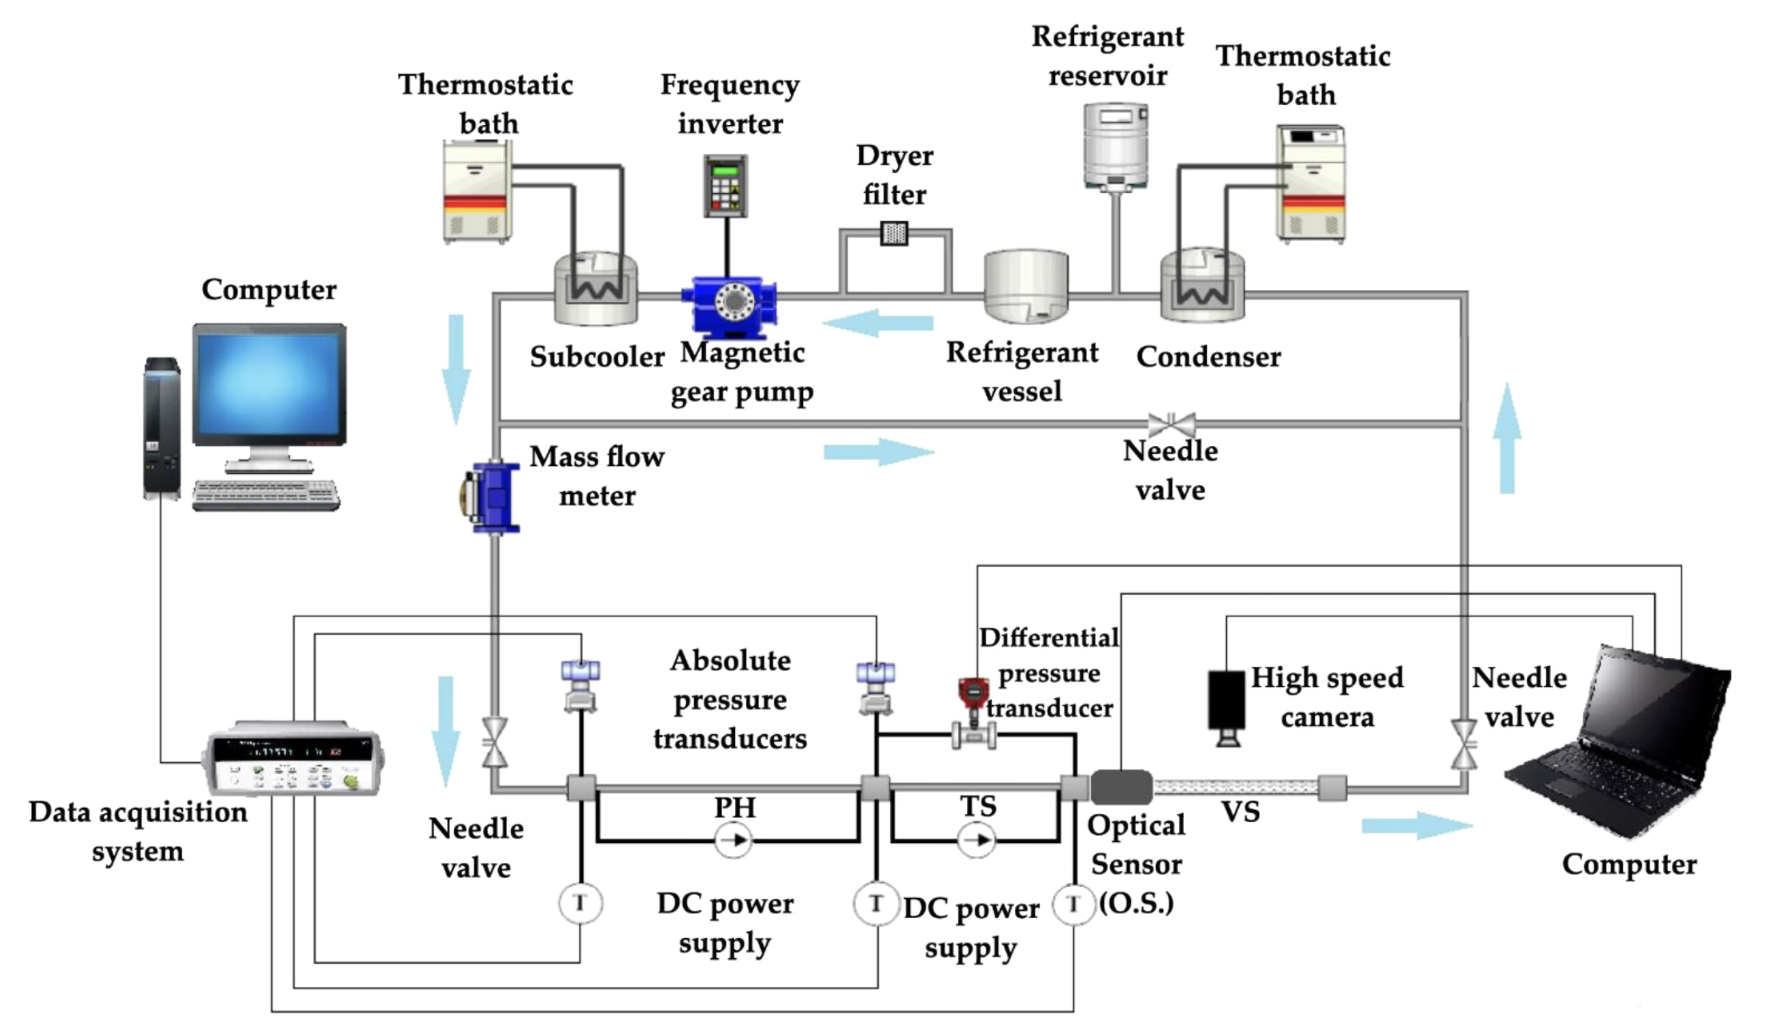
\includegraphics[width=\linewidth]{figuras/deoliveira2021-fig1-arranjo}
  \fonte{Adaptado de \citeonline{deoliveira2021}.}
  \end{minipage}
\end{figure}

\paragraph{Pré-aquecedor e seção de teste.}
O pré-aquecedor (PH) e a seção de teste (TS) são tubos horizontais de aço inoxidável com
diâmetro interno de 1,0\,mm, aquecidos por efeito Joule com aplicação direta de corrente
elétrica controlada por fonte de corrente contínua (SORENSEN\texttrademark{} DCS~8-125E).
O PH tem comprimento total de 515\,mm (440\,mm
aquecidos) e estabelece a condição termodinâmica na entrada da TS. A TS tem comprimento
total de 366\,mm (265\,mm aquecidos). O aquecimento permite estabelecer diferentes
condições de ebulição na saída da TS. A jusante da TS há uma seção de
visualização (VS) de tubo de vidro com 136\,mm e mesmo diâmetro interno, onde os padrões
são registrados visualmente e o sensor óptico é posicionado \cite{deoliveira2019,deoliveira2021}.

\paragraph{Sensor óptico (OS).}
Para a análise temporal dos padrões de escoamento, foi construído um sensor óptico (OS)
que detecta a refração e a variação de luminosidade da luz na interface
líquido-vapor \cite{deoliveira2019}.
Um LED de alta luminosidade ilumina o tubo transversalmente. Um resistor dependente de luz
(LDR) no lado oposto detecta a variação de transmitância óptica causada pela passagem das
fases. A variação de resistência do LDR é convertida em tensão por um circuito com filtro
passa-baixas de quarta ordem e amplificador operacional OPA\,4227, e o sinal é adquirido
pelo módulo NI\,6009 via LabVIEW\,2013. O sensor é posicionado no início da VS, registrando
as condições da saída da TS. Por responder ao que passa pelo feixe do LED em um dado instante,
o OS captura eventos locais associados à morfologia da interface: a passagem de
bolhas e frentes de vapor modifica o sinal. No padrão \textit{dispersed bubbles}, os autores
associaram a resposta do OS à sobreposição dos sinais produzidos pela passagem de várias bolhas
\cite{deoliveira2021}.

\paragraph{Transdutor de pressão diferencial (PD).}
A queda de pressão na TS é medida pelo transdutor ABB\texttrademark{} 600T, com frequência
de resposta de 10\,kHz \cite{deoliveira2021}. O PD mede a diferença de pressão ao
longo da seção de teste, enquanto o OS observa a transmissão óptica na seção de
visualização. Nos ensaios relatados, as frequências características do PD foram
geralmente menores que as do OS \cite{deoliveira2021}. Essa diferença observada
não equivale a uma limitação da frequência nominal de resposta do transdutor.

\paragraph{Aquisição e parâmetros experimentais.}
Nos ensaios de \citeonline{deoliveira2021}, os sinais do OS e do PD foram adquiridos
\textit{simultaneamente} a 1\,kHz, com 8.000 amostras por ensaio (8\,s por condição de operação).
Os padrões também foram registrados na seção de visualização por uma câmera de alta velocidade.
Os parâmetros dos
ensaios de referência estão resumidos no \autoref{qua:params-exp}.

\begin{quadro}[!htbp]
  \centering
  \begin{threeparttable}
  \caption{Parâmetros experimentais dos ensaios de \citeonline{deoliveira2021}.}
  \label{qua:params-exp}
  \begin{tabular}{ll}
    \hline
    \textbf{Parâmetro}                                        & \textbf{Valor(es)}           \\
    \hline
    Fluido de trabalho                                        & R600a (isobutano)            \\
    Temperatura de saturação [\textdegree{}C]                 & 27                           \\
    Fluxo mássico $G$ [kg/(m\textsuperscript{2}s)]           & 380, 510, 640, 760 e 890     \\
    Fluxo de calor na TS $q''$ [kW/m\textsuperscript{2}]     & 1, 5, 10, 20, 40 e 80        \\
    Frequência de aquisição [kHz]                             & 1                            \\
    Amostras por ensaio                                       & 8.000 (8\,s)                 \\
    Frequência de resposta do transdutor PD [kHz]            & 10                           \\
    \hline
  \end{tabular}
  \fonte{\citeonline{deoliveira2021}.}
  \end{threeparttable}
\end{quadro}

As sequências de quadros da câmera de alta velocidade registradas para cada condição de
fluxo mássico $G$ e fluxo de calor $q''$ constituíram os dados utilizados neste trabalho: delas se
reconstruiu o sinal espacial de brilho sobre o qual se calculou a coerência \textit{Wavelet}
alternativa, conforme detalhado no \autoref{cap:metodologia}.

\subsubsection{Padrões de escoamento e suas características}\label{sec:padroes}

Os padrões de escoamento observados no microtubo de 1\,mm com isobutano R600a são
descritos a seguir com base em \citeonline{deoliveira2021} e \citeonline{dias2025knn},
desde \textit{dispersed bubbles} até \textit{wavy annular} e \textit{smooth annular}. As faixas
espectrais apresentadas referem-se aos sinais de PD e OS do primeiro estudo e às
condições nele investigadas.
Neste trabalho, utilizaram-se os padrões da classificação manual dos ensaios.
A \autoref{fig:padroes-escoamento} ilustra cinco desses padrões.

\begin{figure}[!htbp]
  \centering
  \begin{minipage}{0.90\textwidth}
  \caption[Padrões de escoamento observados no LETEF.]{Padrões de escoamento
  observados no LETEF: (a) \textit{dispersed bubbles}, (b) \textit{plug}, (c) \textit{slug},
  (d) \textit{churn} e (e) \textit{wavy annular}.}
  \label{fig:padroes-escoamento}
  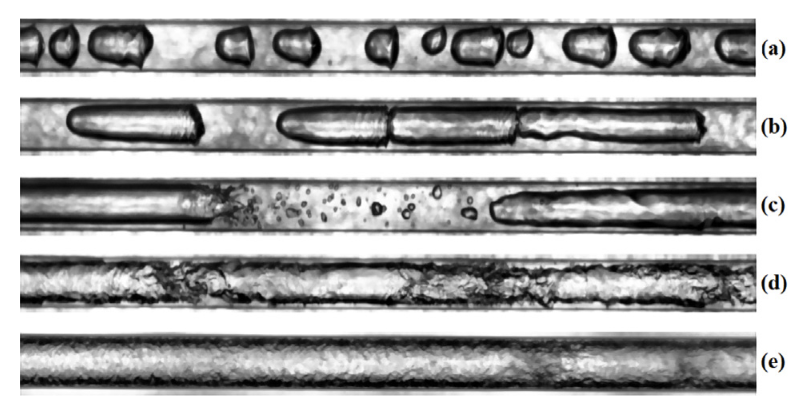
\includegraphics[width=\linewidth]{figuras/dias2025knn-fig4-padroes}
  \fonte{Adaptado de \citeonline{dias2025knn}.}
  \end{minipage}
\end{figure}

\textbf{\textit{Dispersed bubbles}}: esse padrão foi observado com baixo título de vapor $x$,
apenas para o fluxo mássico $G=890\,\text{kg/(m}^2\text{s)}$ e o fluxo de calor
$q''=1\,\text{kW/m}^2$ nos ensaios de \citeonline{deoliveira2021}. Pequenas bolhas ficam
dispersas na fase líquida, com diâmetro menor que o tubo. Nessa condição, o sinal de pressão
diferencial apresentou múltiplos picos entre 6 e 100\,Hz, e o sensor óptico apresentou
energia entre 4 e 35\,Hz. A análise por \textit{Wavelet} mostrou que as frequências
predominantes apareceram de forma intermitente nos dois sinais \cite{deoliveira2021}.

\textbf{\textit{Plug}}: foi observado principalmente em baixos
fluxos de calor $q''$ \cite{deoliveira2021}. As bolhas crescem e assumem forma cilíndrica, com
diâmetro próximo ao do tubo e comprimento maior que o diâmetro, motivo pelo qual esse padrão
também é chamado de \textit{elongated bubble flow} \cite{deoliveira2021}.
Nos ensaios relatados, também ocorreram bolhas dispersas de forma intermitente
entre os \textit{plugs}. As frequências predominantes ficaram entre 0{,}5 e 1\,Hz no PD
e entre 2 e 16\,Hz no OS \cite{deoliveira2021}.

\textbf{\textit{Slug}}: formado pelo coalescimento de \textit{plugs} com o aumento do título de
vapor $x$ e da fração de vazio $\alpha$ nas condições investigadas
\cite{deoliveira2021}. Alterna seções de
líquido e bolsões alongados de vapor com diâmetro próximo ao do tubo
\cite{dias2025knn,deoliveira2021}. A interface é instável e libera
pequenas bolhas dispersas no líquido entre os bolsões. O estudo relatou predominância
de baixas frequências no PD. Para o fluxo mássico $G=510\,\text{kg/(m}^2\text{s)}$, os autores
relataram no OS um pico em 2{,}8\,Hz associado à passagem dos \textit{slugs}. Os autores
sugeriram que as componentes próximas de 8, 12, 23 e 32\,Hz poderiam resultar da passagem
de bolhas dispersas entre os \textit{slugs}. Essas frequências variaram com o fluxo mássico $G$.
A natureza caótica foi indicada pelos maiores expoentes de Lyapunov, positivos, entre 0{,}261
e 0{,}463 no PD e entre 0{,}413 e 4{,}362 no OS \cite{deoliveira2021}.

\textbf{\textit{Churn}}: regime de transição entre \textit{slug} e \textit{annular}
\cite{dias2025knn}.
Nos ensaios de \citeonline{deoliveira2021}, a maior velocidade do vapor foi associada à presença de
jatos e a instabilidades na interface. O sinal de pressão diferencial apresenta
frequências predominantes de baixa energia em 8\,Hz ou menos. No sensor óptico,
observaram-se componentes de baixa frequência e componentes mais altas, entre
15 e 28\,Hz, associadas pelos autores ao aumento do fluxo mássico $G$.


\textbf{\textit{Wavy annular}}: o vapor ocupa o centro
do tubo e o líquido forma um filme na parede
\cite{dias2025knn,deoliveira2021}, sobre o qual deslizam ondas frontais na interface
líquido-vapor \cite{deoliveira2021}. No exemplo analisado pelos autores, a CWT não
identificou frequências características no PD, enquanto o OS apresentou maior energia
entre 2 e 16\,Hz ao longo do tempo.
As flutuações de pressão apresentaram expoente de Hurst abaixo de 0{,}5, indicando
comportamento anti-persistente \cite{deoliveira2021}.

\textbf{\textit{Smooth annular}}: foi observado apenas na combinação
do menor fluxo mássico $G$ com o maior fluxo de calor $q''$ testados
\cite{deoliveira2021}. A interface entre o filme líquido e o núcleo de vapor é
praticamente sem ondas \cite{cheng2023}.
\citeonline{dias2025knn} limitaram a classificação a cinco padrões
de escoamento, não incluindo o \textit{smooth annular}.

As diferenças entre as respostas espectrais do PD e do OS
\cite{deoliveira2021} motivam investigar representações \textit{Wavelet}.
A utilidade da coerência alternativa para os panoramas foi avaliada neste trabalho.



% =========================================================
\subsection{Fração de vazio e representação das fases}\label{sec:fracao-vazio}
% =========================================================

Enquanto o título de vapor $x$ caracteriza a participação do vapor na vazão
mássica, a fração de vazio $\alpha$ expressa a parcela do volume da mistura ocupada
pela fase gasosa. Em escoamento líquido-vapor, essa definição pode ser escrita
como \cite{masiukiewicz2021}:

\begin{equation}\label{eq:fracao-vazio-volume}
  \alpha=\frac{V_v}{V_v+V_l}.
\end{equation}

\noindent
O volume de vapor $V_v$ e o volume de líquido $V_l$ se referem à mesma região
de observação. A fração de vazio $\alpha$ é adimensional: o valor zero
representa somente líquido, e o valor um, somente vapor.

Em uma mesma seção do tubo, a relação entre o título de vapor $x$ e a
fração de vazio $\alpha$ depende das massas específicas e das velocidades médias de cada fase
\cite{deoliveira2021}. A mesma ocupação em volume pode, portanto,
corresponder a participações diferentes na vazão mássica. Por isso, a
proporção de gás identificada nas imagens não determina, por si só,
o título de vapor $x$.

Na análise de imagens, uma máscara binária atribui cada pixel a uma das
fases. A contagem desses pixels fornece uma proporção de área na projeção
observada, como no procedimento de \citeonline{schepperle2024}.
Uma projeção lateral, porém, não informa diretamente a extensão da fase
na profundidade do tubo. A conversão das larguras observadas em áreas de
seções circulares exige uma hipótese geométrica adicional, explicitada na
metodologia. Assim, a estimativa obtida por esse procedimento permanece
condicionada à geometria assumida e à identificação das interfaces.
Os valores de fração de vazio relatados na literatura não foram empregados
como calibração das estimativas obtidas nesse trabalho.

A fração média, isoladamente, não determina a forma ou a distribuição das
estruturas de gás. \citeonline{masiukiewicz2021} destacaram essa limitação ao
combinar a fração volumétrica com parâmetros de tamanho, distribuição e
superfície interfacial. Na análise por \textit{Wavelet},
\citeonline{nguyen2010} também utilizaram a fração de vazio média junto ao
coeficiente de energia \textit{Wavelet} local efetiva na identificação de bolhas discretas
e de casos de \textit{churn}. Esses antecedentes motivam examinar
descritores complementares: a estimativa de fração de vazio resume a
ocupação de vapor, as transições da máscara descrevem as alternâncias
espaciais detectadas e os perfis \textit{Wavelet} caracterizam a distribuição
das variações de intensidade por escala. Essa relação conceitual não
transforma o sinal de intensidade em uma medição calibrada de fração de vazio.

% ---------------------------------------------------------
\subsection{Transformada \textit{Wavelet}}\label{sec:wavelet}
% ---------------------------------------------------------

A transformada \textit{Wavelet} permite examinar como o conteúdo de um sinal
varia ao longo do tempo. Enquanto o espectro de Fourier global resume as
frequências presentes no registro completo, a análise \textit{Wavelet} localiza essas
componentes no sinal. Para isso, utiliza versões dilatadas e deslocadas de uma
função oscilatória localizada, a \textit{Wavelet} mãe. Escalas pequenas favorecem a
localização de variações rápidas. Escalas grandes permitem distinguir melhor
componentes de baixa frequência \cite{torrence1998}. Essa propriedade permite
examinar variações locais nos sinais de escoamento bifásico.
O \autoref{qua:wavelet-fourier} compara as duas transformadas.

\begin{quadro}[!htbp]
  \centering
  \begin{threeparttable}
  \caption{Comparação entre a transformada de Fourier e a transformada \textit{Wavelet}.}
  \label{qua:wavelet-fourier}
  \begin{tabular}{lll}
    \hline
    \textbf{Característica}       & \textbf{Fourier global} & \textbf{\textit{Wavelet} contínua}   \\
    \hline
    Localização temporal          & Não                  & Sim                            \\
    Informação principal          & Espectro global      & Conteúdo por tempo e escala    \\
    Janela de análise              & Registro completo    & Duração variável com a escala  \\
    Variação ao longo do tempo     & Não localizada       & Representada no mapa           \\
    \hline
  \end{tabular}
  \fonte{Adaptado de \citeonline{torrence1998}.}
  \end{threeparttable}
\end{quadro}

\subsubsection{Transformada \textit{Wavelet} Contínua (CWT)}\label{sec:cwt}

A CWT de um sinal $x(t)$ em relação à \textit{Wavelet}-mãe $\psi$ é definida
na forma integral por \cite{schuck2019}:

\begin{equation}\label{eq:cwt}
  W(a, b) = \frac{1}{\sqrt{a}} \int_{-\infty}^{\infty} x(t)\,
  \psi^*\!\left(\frac{t - b}{a}\right) dt,
\end{equation}

\noindent
O coeficiente \textit{Wavelet} $W(a,b)$ quantifica a resposta do sinal à \textit{Wavelet} na escala $a$
e na posição $b$. A escala $a>0$ controla a duração da função de análise,
enquanto a posição $b$ determina onde ela é centrada no sinal. A integral reúne os
produtos entre o sinal e a conjugada complexa dessa função. O fator
$1/\sqrt{a}$ preserva a energia da \textit{Wavelet} ao variar a escala.
Escalas grandes correspondem a baixas frequências, e escalas pequenas,
a altas frequências. A adaptação ao domínio espacial
e a conversão das escalas em comprimentos de onda são descritas na
\autoref{sec:met-wco-morlet}.

O escalograma permite visualizar como o conteúdo do sinal varia ao longo do
tempo e entre escalas \cite{torrence1998}. Exemplos dos padrões
\textit{slug} e \textit{churn} para os dois canais do arranjo experimental
(\autoref{fig:scalogram-slug} a \autoref{fig:scalogram-churn-os}) estão apresentados
na \autoref{sec:wps-wcs-wco}.

A \textit{Wavelet} de Morlet complexa combina oscilações com uma envoltória
gaussiana e pode ser escrita na forma aproximada
\cite{torrence1998,schuck2019}:

\begin{equation}\label{eq:morlet}
  \psi(t) = \pi^{-1/4}\, e^{-t^2/2}\, e^{j\omega_0 t},
\end{equation}

\noindent
em que a coordenada $t$ é adimensional, a unidade imaginária é $j=\sqrt{-1}$ e
o fator $\pi^{-1/4}$ normaliza a energia.
Neste trabalho, adotou-se a frequência angular central adimensional
$\omega_0=6$ nessa forma aproximada
\cite{schuck2019}. Por ser complexa, a Morlet fornece coeficientes com módulo
e fase, permitindo estudar a relação entre dois sinais \cite{torrence1998}.
A \autoref{fig:morlet-mae} apresenta suas partes real e imaginária, cujas
oscilações diminuem em amplitude ao se afastarem da origem.

\begingroup
\setlength{\intextsep}{12pt}
\begin{figure}[!ht]
  \centering
  \caption[\textit{Wavelet} mãe de Morlet complexa utilizada na análise.]{Partes real
  e imaginária da \textit{Wavelet} mãe de Morlet complexa (\autoref{eq:morlet}), com
  $\omega_0=6$, $a=1$ e $b=0$. Eixos adimensionais.}
  \label{fig:morlet-mae}
  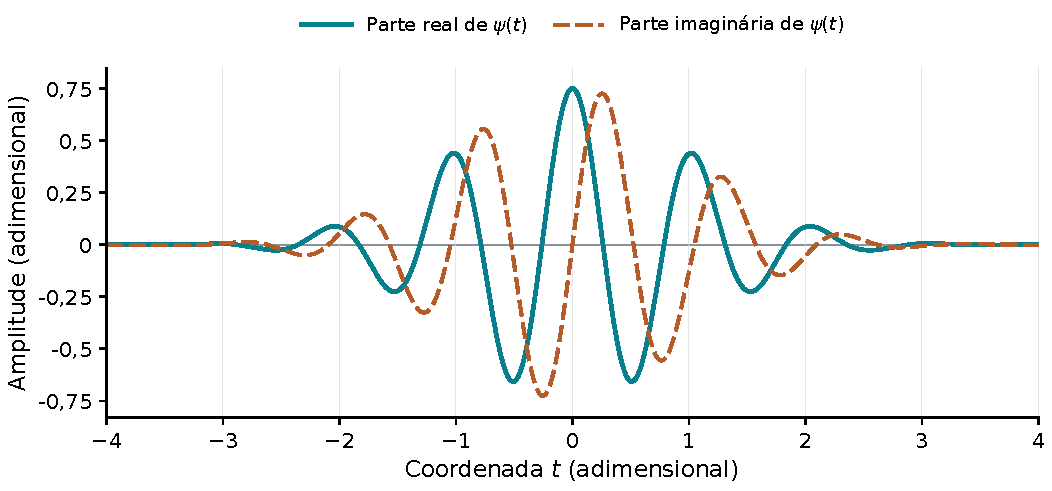
\includegraphics[width=\textwidth]{figuras/morlet_mae.pdf}
  \fonte{Elaborada pelo autor (2026).}
\end{figure}
\endgroup

\subsubsection{Espectro de Potência, Espectro Cruzado e Coerência \textit{Wavelet}}\label{sec:wps-wcs-wco}

A partir da CWT, o espectro de potência descreve as componentes de cada sinal,
o espectro cruzado reúne informações de dois sinais e a coerência quantifica
sua associação por uma medida normalizada \cite{torrence1998}.

\paragraph{Espectro de Potência \textit{Wavelet} (WPS).}
O WPS descreve a distribuição da potência do sinal $x$ entre posições e escalas:

\begin{equation}\label{eq:wps}
  P_x(a, b) = |W_x(a, b)|^2.
\end{equation}

Valores elevados da potência \textit{Wavelet} $P_x(a,b)$ localizam componentes com maior potência
na escala $a$ e na posição $b$.
A média temporal do WPS fornece o espectro \textit{Wavelet} global, comparável a
uma versão suavizada do espectro de Fourier \cite{torrence1998}.

\begingroup
\sloppy
Para ilustrar a interpretação do espectro de potência \textit{Wavelet} $P_x(a,b)$,
apresentam-se os escalogramas de \citeonline{deoliveira2021}, obtidos a partir dos sinais
de pressão diferencial (PD) e do sensor óptico (OS) nos padrões \textit{slug} e
\textit{churn}. Esses mapas mostram como a potência \textit{Wavelet} $P_x(a,b)$
se distribui entre frequências e varia ao longo do tempo.
\par
\endgroup

A \autoref{fig:scalogram-slug} e a \autoref{fig:scalogram-churn} mostram os escalogramas
do WPS do PD para \textit{slug} e \textit{churn}. A \autoref{fig:scalogram-slug-os}
e a \autoref{fig:scalogram-churn-os} apresentam os correspondentes do OS.
Esses exemplos permitem comparar dois padrões pelo mesmo sensor e as respostas
dos dois sensores a um mesmo padrão. Os mapas apresentam distribuições diferentes
de energia e componentes em faixas sobrepostas. O estudo relatou, em geral,
frequências características menores no PD do que no OS \cite{deoliveira2021}.

\begin{figure}[!htbp]
  \centering
  \begin{minipage}{0.85\textwidth}
  \caption[WPS da pressão diferencial no padrão \textit{slug}.]{WPS da pressão
  diferencial em \textit{slug}: (a) sinal e (b, c) escalogramas e perfis de potência
  média. Fluxo mássico $G$ ($\mathrm{kg\,m^{-2}\,s^{-1}}$): (a, c) 760 e (b) 510.}
  \label{fig:scalogram-slug}
  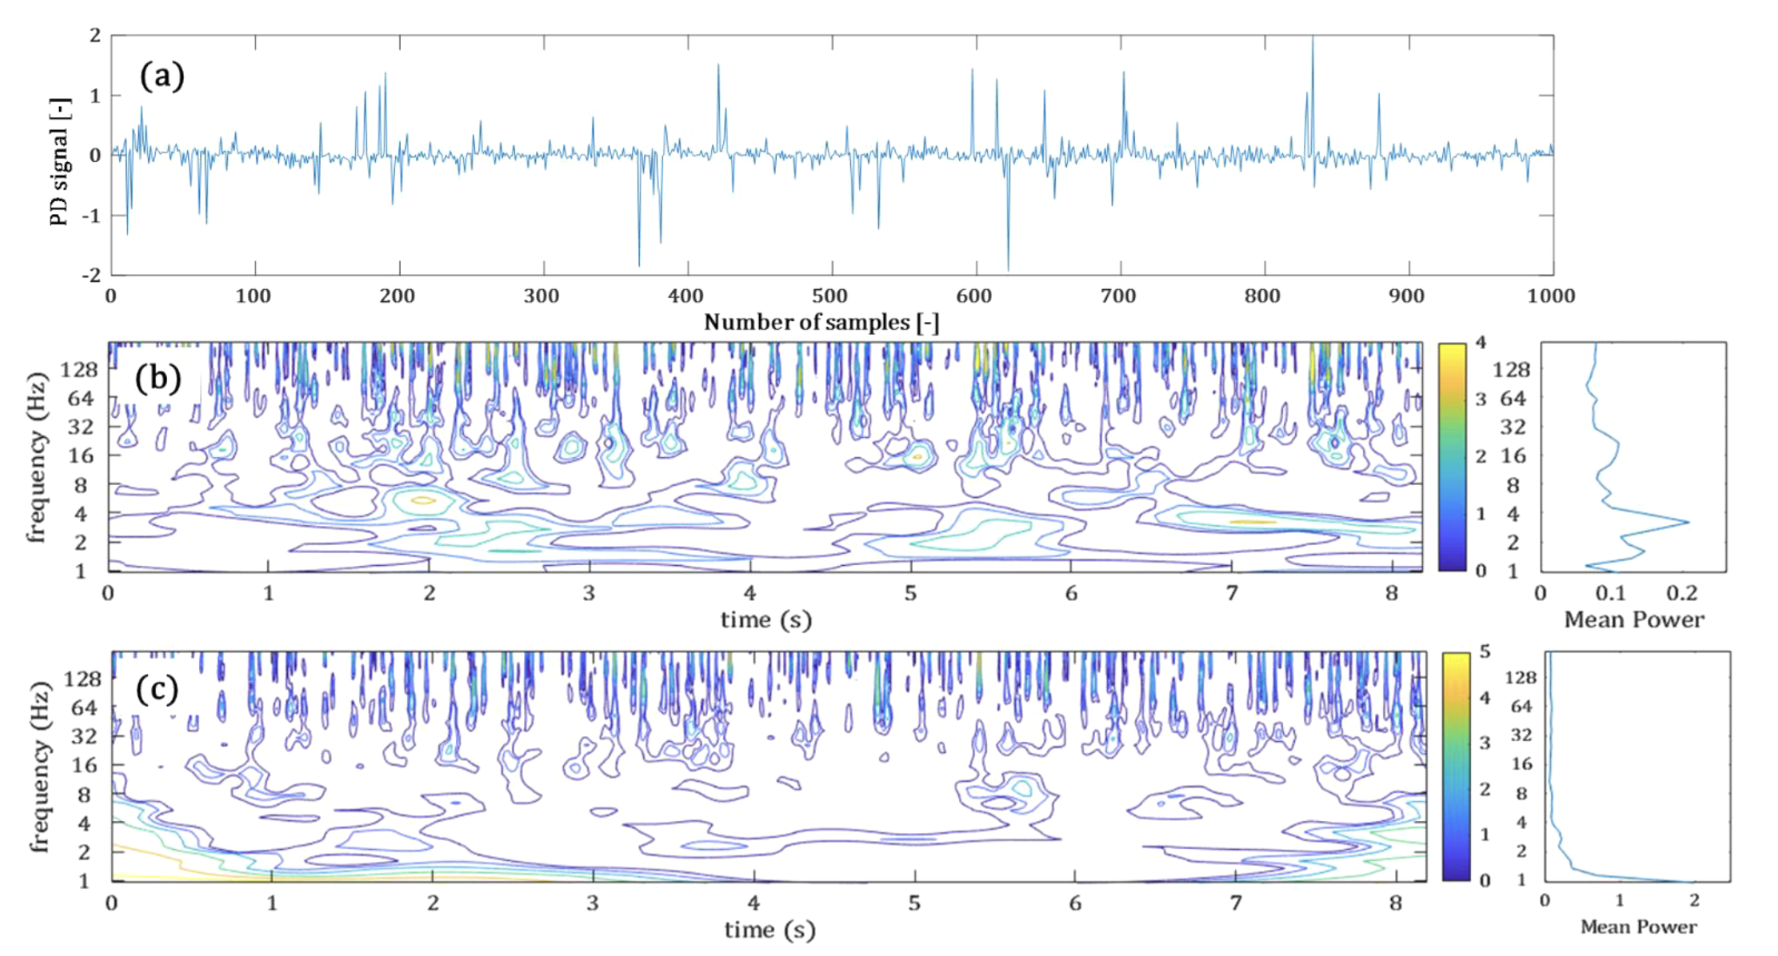
\includegraphics[width=\linewidth]{figuras/deoliveira2021-fig13-slug-pd}
  \fonte{Adaptado de \citeonline{deoliveira2021}.}
  \end{minipage}
\end{figure}

\begin{figure}[!htbp]
  \centering
  \begin{minipage}{0.85\textwidth}
  \caption[WPS do sensor óptico no padrão \textit{slug}.]{WPS do sensor óptico
  em \textit{slug}: (a) sinal e (b, c) escalogramas e perfis de potência média.
  Fluxo mássico $G$ ($\mathrm{kg\,m^{-2}\,s^{-1}}$): (a, c) 760 e (b) 510.}
  \label{fig:scalogram-slug-os}
  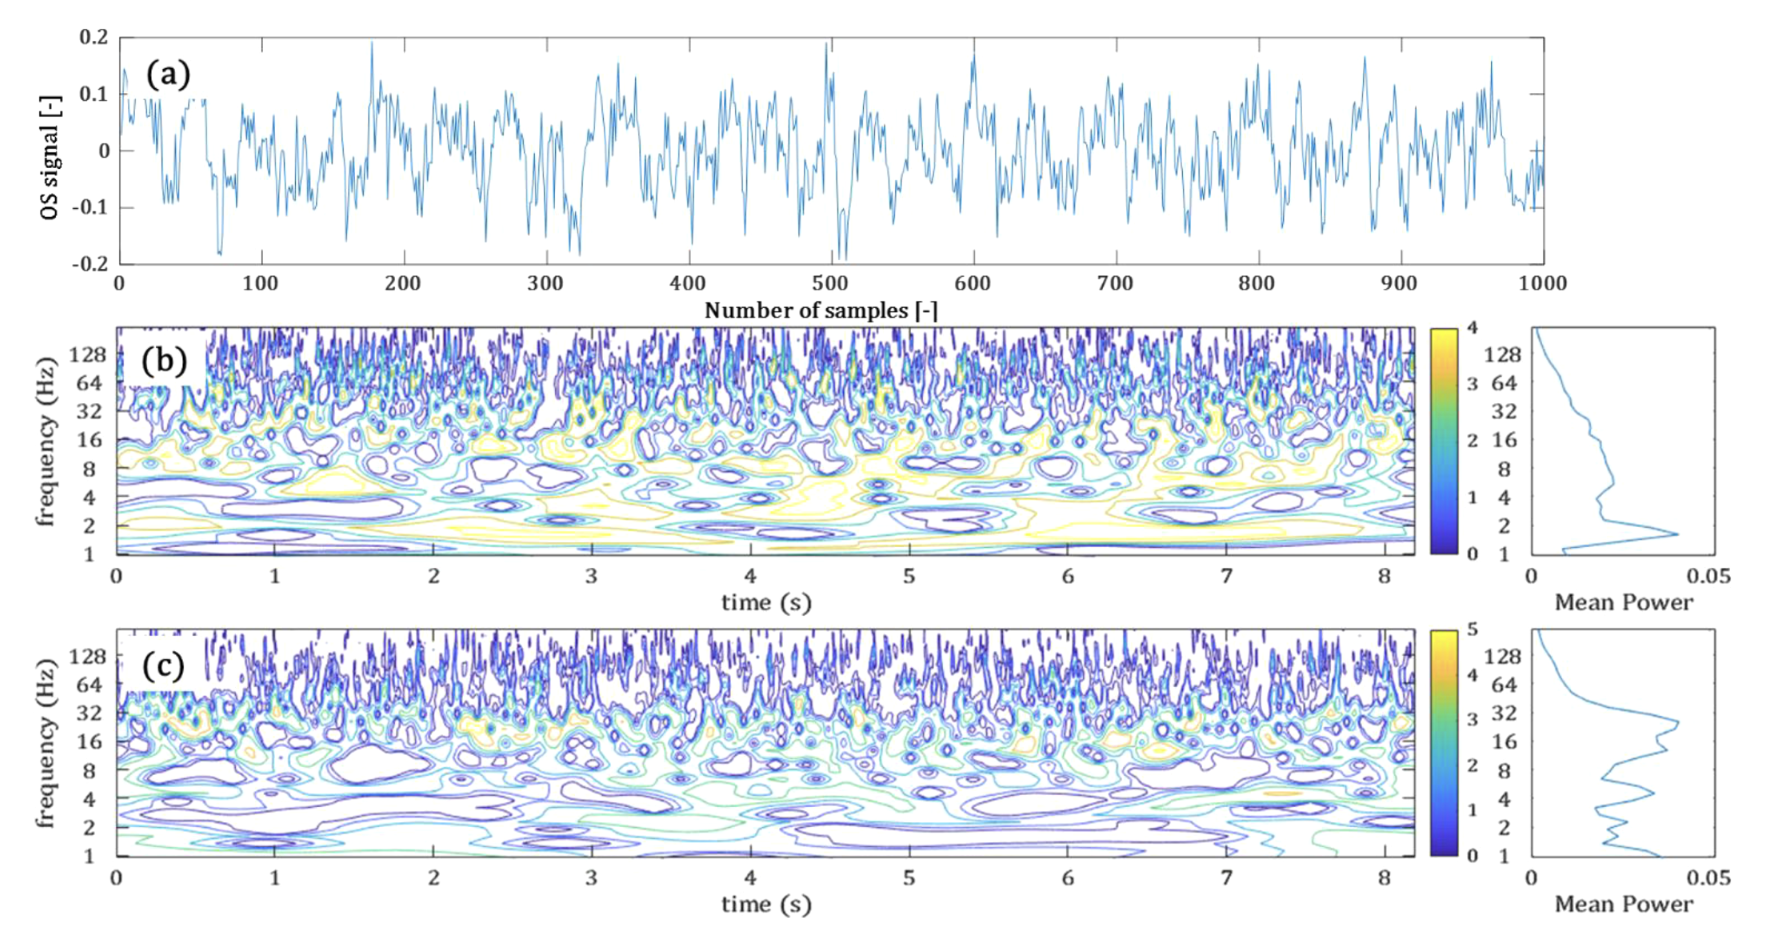
\includegraphics[width=\linewidth]{figuras/deoliveira2021-fig14-slug-os}
  \fonte{Adaptado de \citeonline{deoliveira2021}.}
  \end{minipage}
\end{figure}

\begin{figure}[!htbp]
  \centering
  \begin{minipage}{0.85\textwidth}
  \caption[WPS da pressão diferencial no padrão \textit{churn}.]{WPS da pressão
  diferencial em \textit{churn}: (a) sinal e (b, c) escalogramas e perfis de potência
  média. Fluxo mássico $G$ ($\mathrm{kg\,m^{-2}\,s^{-1}}$): (a, b) 510 e (c) 760.}
  \label{fig:scalogram-churn}
  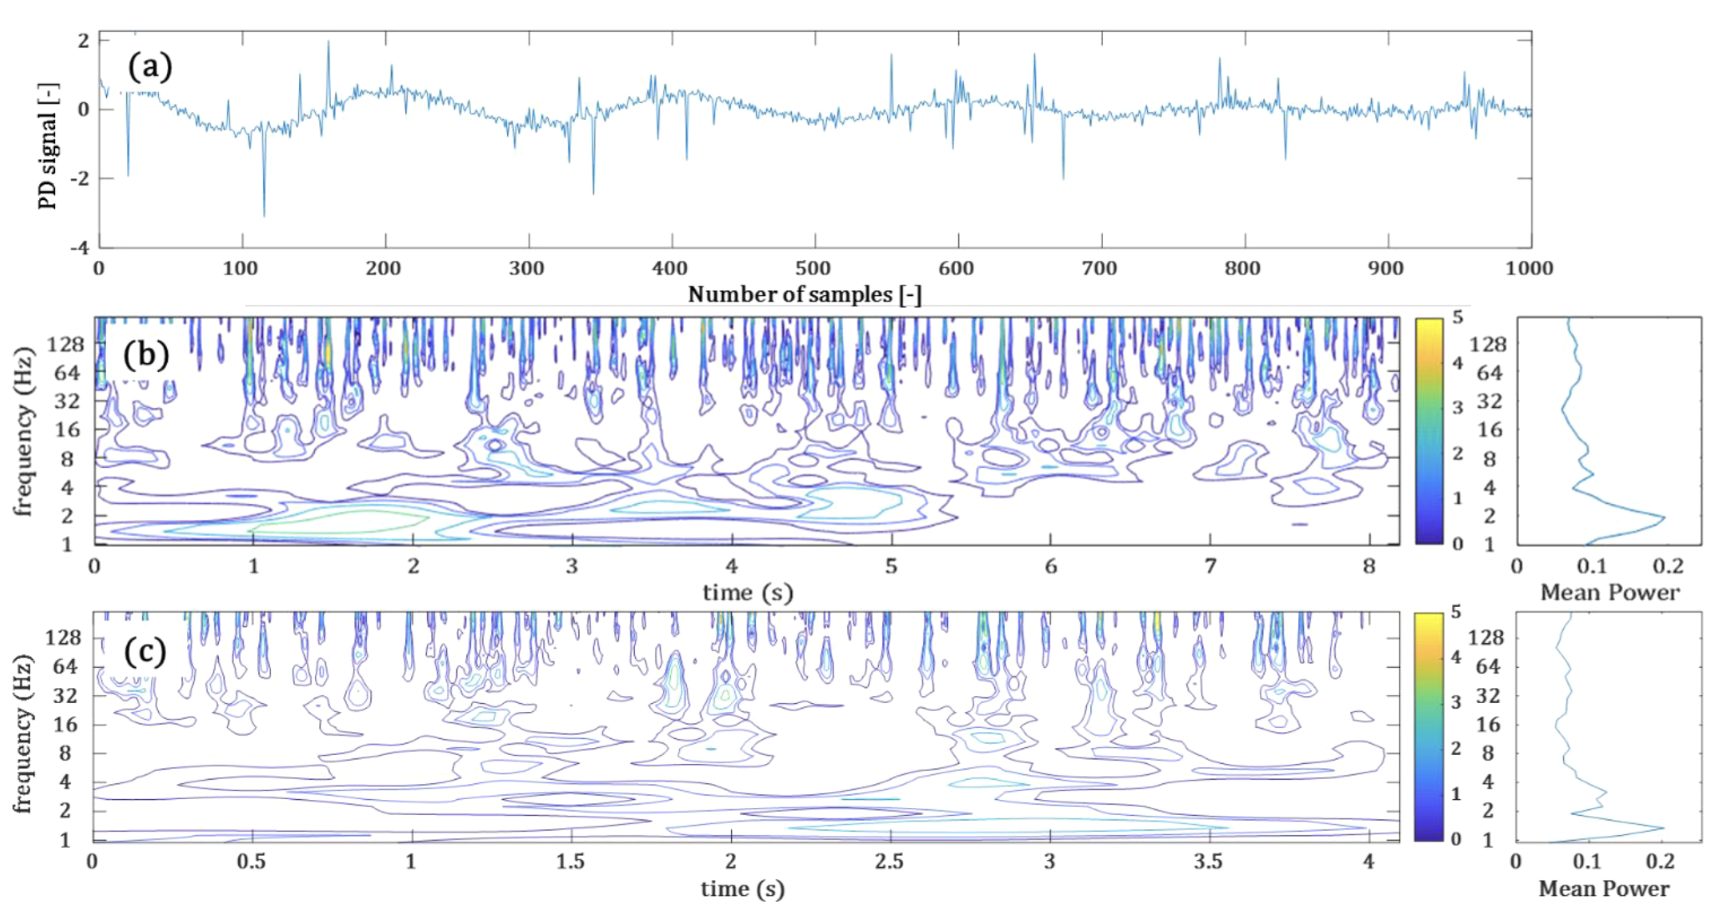
\includegraphics[width=\linewidth]{figuras/deoliveira2021-fig17-churn-pd}
  \fonte{Adaptado de \citeonline{deoliveira2021}.}
  \end{minipage}
\end{figure}

\begin{figure}[!htbp]
  \centering
  \begin{minipage}{0.85\textwidth}
  \caption[WPS do sensor óptico no padrão \textit{churn}.]{WPS do sensor óptico
  em \textit{churn}: (a) sinal e (b, c) escalogramas e perfis de potência média.
  Fluxo mássico $G$ ($\mathrm{kg\,m^{-2}\,s^{-1}}$): (b) 510 e (c) 760.}
  \label{fig:scalogram-churn-os}
  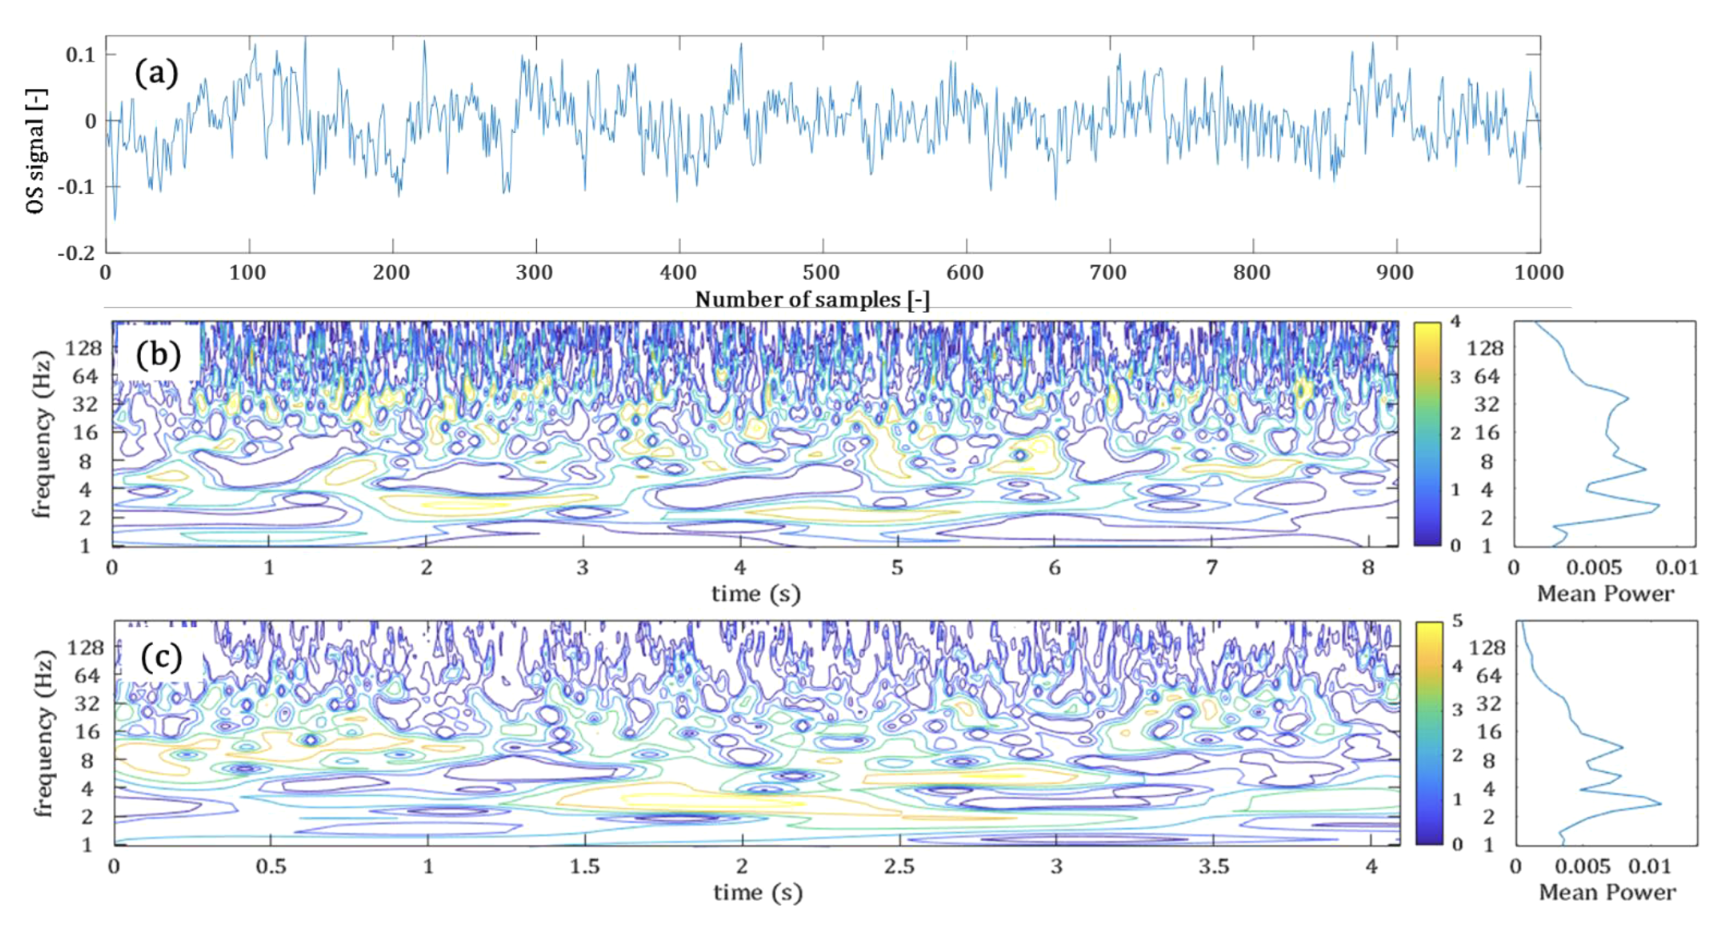
\includegraphics[width=\linewidth]{figuras/deoliveira2021-fig18-churn-os}
  \fonte{Adaptado de \citeonline{deoliveira2021}.}
  \end{minipage}
\end{figure}


\paragraph{Espectro Cruzado \textit{Wavelet} (WCS).}
O WCS mede a relação entre dois sinais $x$ e $y$ no domínio tempo-escala:

\begin{equation}\label{eq:wcs}
  C_{xy}(a, b) = W_x(a, b) \cdot W_y^*(a, b).
\end{equation}

O produto combina os coeficientes dos dois sinais na mesma escala e posição.
Seu módulo destaca regiões de potência comum, e sua fase descreve a defasagem
relativa entre as componentes \cite{torrence1998,grinsted2004}.
Como o WCS ainda depende das amplitudes dos sinais, potência comum elevada
não equivale, por si só, a coerência elevada. A conversão da diferença de
fase em atraso temporal depende da frequência analisada \cite{grinsted2004}.

\paragraph{Coerência \textit{Wavelet} (WCO).}
A coerência \textit{Wavelet} clássica $\gamma_{xy}$ é uma medida quadrática de associação,
com valores entre 0 e 1 quando o denominador é positivo:

\begin{equation}\label{eq:wco-classica}
  \gamma_{xy}(a, b) = \frac{|S\bigl[a^{-1}C_{xy}(a, b)\bigr]|^2}
                           {S\bigl[a^{-1}P_x(a, b)\bigr] \cdot S\bigl[a^{-1}P_y(a, b)\bigr]},
\end{equation}

\noindent
A normalização compara o espectro cruzado \textit{Wavelet} $C_{xy}(a,b)$ com os
espectros de potência \textit{Wavelet} $P_x(a,b)$ e $P_y(a,b)$, considerando a potência
presente em cada sinal. A suavização $S[\cdot]$ calcula médias ponderadas em uma
pequena região do mapa, reunindo instantes próximos e escalas semelhantes.
Antes dessas médias, aplica-se o fator de ponderação $a^{-1}$, correspondente ao
inverso da escala $a$. Assim, a coerência \textit{Wavelet} clássica $\gamma_{xy}(a,b)$
descreve a associação entre as oscilações dos dois sinais nessa região.
Valores da coerência \textit{Wavelet} clássica $\gamma_{xy}(a,b)$ próximos de 1 indicam
forte associação linear local, enquanto valores da coerência \textit{Wavelet}
clássica $\gamma_{xy}(a,b)$ próximos de zero indicam associação linear local fraca
\cite{grinsted2004}.

\paragraph{Formulação alternativa de Schuck e Bodmann.}

Sem a suavização $S[\cdot]$, a coerência \textit{Wavelet} clássica $\gamma_{xy}(a,b)$
seria calculada isoladamente em cada ponto do mapa. Nesse caso, a identidade
$|W_xW_y^*|^2=|W_x|^2|W_y|^2$ faria o numerador e o denominador da
\autoref{eq:wco-classica} terem o mesmo valor. A divisão resultaria, portanto, em 1
sempre que o denominador fosse diferente de zero, mesmo para sinais sem relação
física entre si. Esse resultado decorreria da própria fórmula e não demonstraria
uma associação entre os sinais \cite{torrence1998}. Ao reunir valores vizinhos antes
da divisão, a suavização $S[\cdot]$ evita esse resultado automaticamente igual a 1.
A coerência \textit{Wavelet} clássica $\gamma_{xy}(a,b)$ passa, então, a representar a
associação em uma pequena região de tempo e escala ao redor de cada ponto
\cite{grinsted2004}.

\citeonline{schuck2019} formularam uma alternativa baseada na CWT das funções de
correlação. Para processos estacionários, definiram a autocorrelação e a correlação
cruzada pela esperança matemática:

\begin{equation}\label{eq:autocorr}
  R_{xx}(\tau)=\operatorname{E}\{x(t+\tau)x^*(t)\},
\end{equation}

\begin{equation}\label{eq:crosscorr}
  R_{xy}(\tau)=\operatorname{E}\{x(t+\tau)y^*(t)\}.
\end{equation}

\noindent
A autocorrelação $R_{xx}(\tau)$ compara um sinal com uma versão deslocada
de si mesmo, enquanto a correlação cruzada $R_{xy}(\tau)$ compara dois sinais
separados pelo atraso $\tau$. A esperança matemática $\operatorname{E}\{\cdot\}$
representa a média estatística teórica desses produtos, com o conjugado complexo
do segundo fator. Sob a hipótese de estacionariedade, essas funções
dependem do atraso, sem depender da origem temporal $t$ \cite{schuck2019}.

Neste trabalho, as autocorrelações estimadas $\widehat R_{xx}$ e
$\widehat R_{yy}$ e a correlação cruzada estimada $\widehat R_{xy}$ foram
calculadas com um registro de cada sinal por comparação. O chapéu indica
que esses valores foram estimados a partir dos dados. Aplicou-se então a CWT
a essas funções, seguindo a formulação de \citeonline{schuck2019}:

\begin{equation}\label{eq:wps-alt}
  \widetilde P_x(a,b)=\left|W_{\widehat R_{xx}}(a,b)\right|,
  \qquad
  \widetilde P_y(a,b)=\left|W_{\widehat R_{yy}}(a,b)\right|,
\end{equation}

\begin{equation}\label{eq:wcs-alt}
  \widetilde C_{xy}(a,b)=W_{\widehat R_{xy}}(a,b),
\end{equation}

\begin{equation}\label{eq:wco-alt}
  \widetilde\gamma_{xy}(a,b)=
  \frac{|\widetilde C_{xy}(a,b)|^2}
       {\widetilde P_x(a,0)\,\widetilde P_y(a,0)}.
\end{equation}

\noindent
O coeficiente \textit{Wavelet} $W_{\widehat R_{xx}}(a,b)$ resulta da CWT da
autocorrelação estimada $\widehat R_{xx}$. Seu módulo fornece a potência
alternativa $\widetilde P_x(a,b)$, com cálculo análogo para a potência
alternativa $\widetilde P_y(a,b)$. A escala $a$ controla a dilatação da
\textit{Wavelet}, enquanto a posição $b$ indica onde ela é centrada no eixo
do atraso da correlação $\tau$. A CWT da correlação cruzada estimada $\widehat R_{xy}$
fornece o espectro cruzado complexo $\widetilde C_{xy}(a,b)$, que conserva
módulo e fase \cite{schuck2019}.

Na \autoref{eq:wco-alt}, divide-se o módulo ao quadrado do espectro cruzado
alternativo $\widetilde C_{xy}(a,b)$ pelo produto das potências alternativas
$\widetilde P_x(a,0)$ e $\widetilde P_y(a,0)$. Esses valores correspondem à
mesma escala $a$ e ao atraso nulo $b=0$, onde ocorrem os máximos com a Morlet
adotada. A coerência alternativa $\widetilde\gamma_{xy}(a,b)$ só é definida
quando esse produto é positivo. O mapa descreve a associação por escala $a$
e atraso relativo $b$, sem localizar o instante original de ocorrência de
um evento \cite{schuck2019}. Na aplicação deste trabalho, o atraso $b$ foi
expresso em pixels do panorama reconstruído.

A formulação pressupõe processos estacionários e depende das correlações
estimadas a partir dos registros disponíveis. A aplicação da CWT a essas
correlações dispensa a suavização da definição clássica, mas mantém a
incerteza associada à estimação \cite{schuck2019}. O procedimento discreto
adotado neste trabalho é apresentado na \autoref{sec:met-wco}.

O \autoref{qua:wco-comparativo} resume as diferenças relevantes para a leitura
dos mapas.

\begin{quadro}[!htbp]
  \centering
  \begin{threeparttable}
  \caption[Comparação entre as formulações clássica e alternativa da coerência
  \textit{Wavelet}.]{Formulações clássica e alternativa da coerência
  \textit{Wavelet}, conforme \citeonline{torrence1998},
  \citeonline{grinsted2004} e \citeonline{schuck2019}.}
  \label{qua:wco-comparativo}
  \begin{tabular}{p{3.1cm}p{5.1cm}p{5.1cm}}
    \hline
    \textbf{Aspecto} & \textbf{Clássica} & \textbf{Alternativa} \\
    \hline
    Entrada da CWT & Sinais diretamente & Funções de correlação estimadas \\
    Potência & $|W_x(a,b)|^2$ & $|W_{\widehat R_{xx}}(a,b)|$ \\
    Espectro cruzado & $W_x(a,b)W_y^*(a,b)$ & $W_{\widehat R_{xy}}(a,b)$ \\
    Normalização & Espectros suavizados em tempo e escala & Potências no atraso nulo da mesma escala \\
    Coordenada $b$ & Posição no sinal & Atraso da correlação \\
    Interpretação & Associação localizada no tempo & Associação por escala e atraso \\
    \hline
  \end{tabular}
  \fonte{Elaborada pelo autor (2026).}
  \end{threeparttable}
\end{quadro}

\citeonline{schuck2019} avaliaram a formulação com sinais sintéticos contendo
pulsos gaussianos modulados e ruído gaussiano, com razão sinal-ruído de 5\,dB e
atraso conhecido de 500 amostras entre os pulsos. Nos exemplos apresentados,
a formulação alternativa permitiu identificar o atraso e a escala dos
transientes mesmo na presença de eventos adicionais não correlacionados.

Neste trabalho, a formulação foi aplicada aos sinais de intensidade extraídos
dos panoramas. Essa aplicação exigiu considerar as condições de reconstrução
das imagens, pois as emendas entre as tiras de quadros podem introduzir
variações no sinal analisado. O \autoref{cap:metodologia} apresenta o
procedimento de reconstrução dos panoramas e as etapas de análise desses sinais.


\chapter{Metodologia}\label{cap:metodologia}

Este capítulo descreve a abordagem adotada para investigar a aplicabilidade da coerência
\textit{Wavelet} alternativa de \citeonline{schuck2019} como ferramenta de caracterização
dos padrões de escoamento bifásico no arranjo experimental do LETEF.
Em vez de utilizar os sinais dos sensores no domínio do tempo, o método construiu, para
cada ensaio, um sinal unidimensional de brilho no domínio \textit{espacial}, obtido a
partir de um panorama reconstruído das imagens da câmera de alta velocidade, e aplicou a
formulação de \citeonline{schuck2019} a pares desses sinais.
A \autoref{sec:met-visao} apresenta uma visão geral do método; as seções seguintes
descrevem os dados, o pré-processamento, o cálculo da coerência e a análise das
assinaturas espectrais, comparando os campos WPS, WCS e WCO entre ensaios de um mesmo
padrão (repetibilidade intra-padrão) e entre padrões distintos (separação inter-padrão).

% =========================================================
\section{Visão geral do método proposto}\label{sec:met-visao}
% =========================================================

A abordagem consiste em calcular a coerência \textit{Wavelet} alternativa
$\widetilde{\gamma}_{xy}(a)$ entre dois sinais espaciais de brilho $x$ e $y$, cada um
extraído do panorama reconstruído de um ensaio, e verificar se as assinaturas espectrais
resultantes são reprodutíveis dentro de um mesmo padrão de escoamento e distinguíveis
entre padrões distintos. Os dois sinais comparados são \textit{dois ensaios} (\textit{runs}):
no modo intra-padrão, dois ensaios do mesmo padrão, para avaliar a repetibilidade; no modo
inter-padrão, ensaios de padrões diferentes, para avaliar a separação. A hipótese investigada
é se a estrutura espectral do acoplamento, expressa por $\widetilde{\gamma}_{xy}(a)$ em
função da escala, se mantém consistente entre ensaios de um mesmo padrão e varia
sistematicamente de um padrão para outro, refletindo a dinâmica distinta da interface
líquido-vapor em cada regime. A coerência $\widetilde{\gamma}_{xy}(a)$ é o descritor
principal; o perfil de potência média $|\text{WPS}|$ por comprimento de onda complementa
a análise.

O \textit{pipeline} é composto pelas seguintes etapas:

\begin{enumerate}
  \item construção do sinal espacial de brilho a partir do panorama de cada ensaio;
  \item pré-processamento dos sinais;
  \item cálculo da autocorrelação de cada ensaio e da correlação cruzada entre os dois
        ensaios;
  \item aplicação da CWT nas funções de correlação e obtenção de
        $\widetilde{P}_x(a)$, $\widetilde{P}_y(a)$, $\widetilde{C}_{xy}(a)$ e da coerência
        alternativa $\widetilde{\gamma}_{xy}(a)$ no atraso nulo;
  \item análise das assinaturas espectrais (campos WCO e WCS e perfil de potência média)
        por padrão de escoamento, nos modos intra-padrão e inter-padrão.
\end{enumerate}

A \autoref{fig:pipeline} resume esquematicamente o fluxo de processamento.

\begin{figure}[htb]
  \centering
  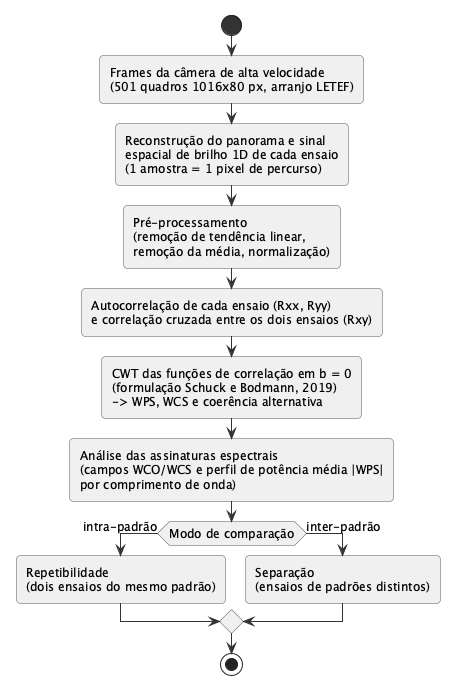
\includegraphics[width=0.55\textwidth]{figuras/pipeline-wco}
  \caption{Fluxograma do método para caracterização dos padrões de escoamento
           por coerência \textit{Wavelet} alternativa a partir de sinais espaciais de brilho.}
  \label{fig:pipeline}
  \fonte{Elaborado pelo autor.}
\end{figure}

% =========================================================
\section{Dados experimentais}\label{sec:met-dados}
% =========================================================

Os dados utilizados neste trabalho são os quadros (\textit{frames}) da câmera de alta
velocidade registrados por \citeonline{deoliveira2021} no arranjo experimental do LETEF,
descrito na \autoref{sec:arranjo}. O fluido estudado é o isobutano (R600a), a
27\textdegree{}C de temperatura de saturação. Cada ensaio corresponde a uma sequência de
501 quadros de $1016 \times 80$ pixels, registrados na seção de visualização para uma
combinação específica de fluxo mássico $G$ e fluxo de calor $q''$, abrangendo as seis
condições de padrão de escoamento identificadas naquele trabalho: bolha dispersa,
\textit{plug}, \textit{slug}, \textit{churn}, anular ondulado e anular liso.

A partir de cada sequência de quadros, reconstruiu-se um panorama do escoamento. Para cada
par de quadros consecutivos mediu-se o deslocamento horizontal do escoamento por correlação
cruzada dos perfis de brilho médios da banda central do tubo; costurou-se, então, uma tira
central de cada quadro na posição medida, formando uma imagem panorâmica cuja largura é o
deslocamento acumulado ao longo do ensaio. O panorama bidimensional foi colapsado em um
sinal unidimensional pela média das colunas, em duas variantes: a média das linhas 20 a 59
(núcleo do escoamento, denominada \textit{cropped}) e a linha central 40 (\textit{center}).
No sinal resultante, uma amostra corresponde a um pixel de percurso do escoamento no tubo:
trata-se, portanto, de um sinal puramente \textit{espacial}, sem eixo de tempo nem
frequência de amostragem associada.

A escolha do domínio espacial em vez do domínio do tempo decorre do número de amostras
disponível. No domínio do tempo, cada ensaio dispõe de apenas 501 quadros; a série temporal
efetivamente reamostrada usada como contraparte neste trabalho reduz-se a cerca de 287
amostras. Já o panorama espacial reconstruído contém, conforme o ensaio, de algumas centenas
a mais de vinte mil pixels de percurso, situando-se tipicamente na faixa de milhares de
amostras (por exemplo, os ensaios de \textit{churn} analisados têm entre 7\,584 e 9\,586
pixels). O sinal espacial oferece, assim, uma ou duas ordens de grandeza mais amostras do
que a série temporal, o que se traduz em maior resolução espectral e na ausência de um teto
de Nyquist atrelado à taxa de quadros da câmera, condição vantajosa para a estimativa das
funções de correlação exigidas pela formulação de \citeonline{schuck2019}.

Para cada ensaio, o padrão de escoamento foi previamente identificado por análise visual
das imagens da câmera de alta velocidade na seção de visualização, conforme descrito por
\citeonline{deoliveira2021}. Essa identificação prévia constitui o rótulo de referência
utilizado para avaliar se as assinaturas de coerência \textit{Wavelet} correspondem a cada
padrão. Entre os padrões, apenas o \textit{churn} ($n = 10$) e o anular ondulado ($n = 9$)
dispõem de ensaios suficientes para sustentar a análise de repetibilidade intra-padrão; os
demais (\textit{plug}, \textit{slug} e \textit{slug}--\textit{churn}) têm $n \leq 4$ e são
tratados de forma ilustrativa.

A comparação foi feita em dois modos, ambos restritos aos cinco padrões com pelo menos dois
ensaios (\textit{churn}, com dez ensaios; anular ondulado, com nove; \textit{plug}, com quatro;
\textit{slug}, com três; e \textit{slug}--\textit{churn}, com dois), que somam vinte e oito
ensaios. Os padrões com um único ensaio (bolha dispersa, anular liso e \textit{plug}--\textit{slug})
ficaram de fora por não formarem pares. No modo intra-padrão, avaliaram-se todas
as combinações de dois ensaios de um mesmo padrão, o que dá noventa e um pares (quarenta e cinco
de \textit{churn}, trinta e seis de anular ondulado, seis de \textit{plug}, três de \textit{slug}
e um de \textit{slug}--\textit{churn}). No modo inter-padrão, formaram-se os pares de ensaios de
padrões distintos, ou seja, o produto cartesiano dos ensaios de cada par de padrões, chegando-se
a duzentos e oitenta e sete pares de ensaios repartidos pelas dez combinações possíveis dos cinco
padrões. A ordem dentro de cada par define apenas qual ensaio entra como primeiro sinal
(prioridade \textit{churn}, anular ondulado e, para os demais, ordem alfabética); como a coerência
é definida por escala, essa ordem não altera seu valor. Ambos os modos empregam o cálculo de
coerência \textit{Wavelet} alternativa descrito nas seções seguintes, diferindo apenas na regra de
emparelhamento dos ensaios.

% =========================================================
\section{Pré-processamento dos sinais}\label{sec:met-preproc}
% =========================================================

Antes de calcular as funções de correlação, cada sinal espacial passou pelas seguintes
etapas de pré-processamento:

\begin{enumerate}
  \item Remoção de tendência: subtração de uma tendência linear ajustada ao sinal, para
        eliminar derivas de baixa frequência introduzidas por variações lentas de
        iluminação e pela costura do panorama, que não carregam informação sobre a
        morfologia do escoamento;
  \item Remoção da média: subtração do valor médio, eliminando a componente contínua e
        garantindo que a autocorrelação seja bem definida;
  \item Normalização: divisão pelo desvio padrão amostral, garantindo variância unitária
        e tornando as funções de correlação comparáveis entre ensaios com diferentes
        condições operacionais. A formulação de \citeonline{schuck2019} pressupõe que os
        sinais sejam realizações de processos estacionários, hipótese sob a qual as funções
        de auto e correlação cruzada estão bem definidas.
\end{enumerate}

A formulação alternativa de \citeonline{schuck2019} pressupõe processos estacionários.
No domínio espacial, essa hipótese equivale à homogeneidade estatística do panorama ao
longo do eixo de percurso: como cada ensaio de \citeonline{deoliveira2021} foi coletado com
$G$ e $q''$ fixos, em regime estabelecido, o padrão de escoamento mantém-se estatisticamente
uniforme ao longo do trecho reconstruído, conforme o protocolo experimental descrito na
\autoref{sec:arranjo}.

% =========================================================
\section{Cálculo da coerência \textit{Wavelet} alternativa}\label{sec:met-wco}
% =========================================================

O cálculo da coerência \textit{Wavelet} alternativa seguiu a formulação de
\citeonline{schuck2019}, conforme descrita na \autoref{sec:wps-wcs-wco}. As etapas foram
as seguintes:

\begin{enumerate}
  \item Autocorrelação e correlação cruzada: calcularam-se numericamente a autocorrelação
        do primeiro ensaio $R_{xx}(\tau)$, a autocorrelação do segundo ensaio
        $R_{yy}(\tau)$ e a correlação cruzada entre os dois ensaios $R_{xy}(\tau)$ a partir
        dos sinais espaciais pré-processados, para defasagens $\tau$ de $-(N-1)$ a $N-1$
        pixels, em que $N$ é o comprimento do sinal (variável de um ensaio para outro, da
        ordem de milhares de pixels), com normalização enviesada, dividindo cada soma por
        $N$;
  \item CWT das funções de correlação: aplicou-se a CWT de \textit{Wavelet} de Morlet
        complexa a cada função de correlação, avaliada em $b = 0$, sobre uma grade
        logarítmica de 200 escalas cobrindo comprimentos de onda de 50 a 3\,000 pixels,
        faixa escolhida para englobar as estruturas espaciais características dos padrões
        de escoamento. A realização concreta empregou a \textit{Wavelet} \texttt{cmor2.0-0.9549}
        da biblioteca \textit{PyWavelets} (largura de banda 2,0 e frequência central
        0,9549), conforme detalhado na \autoref{sec:met-wco-morlet};
  \item Espectros alternativos: calcularam-se o espectro de potência alternativo do
        primeiro ensaio $\widetilde{P}_x(a) = |W_{R_{xx}}(a,0)|$, o do segundo ensaio
        $\widetilde{P}_y(a) = |W_{R_{yy}}(a,0)|$ e o espectro cruzado alternativo
        $\widetilde{C}_{xy}(a) = |W_{R_{xy}}(a,0)|$, conforme as \autoref{eq:wps-alt} e
        \autoref{eq:wcs-alt};
  \item Coerência por escala: obteve-se a coerência \textit{Wavelet} alternativa
        $\widetilde{\gamma}_{xy}(a) = \widetilde{C}_{xy}(a)^2\,/\,[\widetilde{P}_x(a)\cdot\widetilde{P}_y(a)]$
        (\autoref{eq:wco-alt}), avaliada no atraso nulo, resultando em uma curva de
        coerência em função do comprimento de onda de cada escala.
\end{enumerate}

A implementação foi realizada em Python, com as bibliotecas \textit{NumPy} e \textit{SciPy}
para os cálculos de correlação e \textit{PyWavelets} (\textit{pywt}) para a CWT. Antes da
aplicação aos dados reais, a implementação foi validada com sinais sintéticos de frequência,
fase e razão sinal-ruído controladas, seguindo o procedimento descrito por
\citeonline{schuck2019}, para confirmar que as equações estão corretamente implementadas e
que o método recupera os resultados esperados.

\subsection{Parametrização da \textit{Wavelet} de Morlet}\label{sec:met-wco-morlet}

A moldura teórica da \autoref{sec:cwt} descreve a \textit{Wavelet} de Morlet complexa pela
frequência central adimensional $\omega_0 = 6$. A implementação usou a \textit{Wavelet}
complexa de Morlet \texttt{cmor2.0-0.9549} do \textit{PyWavelets}, cujos parâmetros de
largura de banda (2,0) e de frequência central (0,9549) definem a realização discreta
concreta dessa família. A conversão entre escala $a$ e comprimento de onda $\lambda$ segue
a frequência central da \textit{Wavelet}, obtida por \texttt{pywt.central\_frequency}, de
modo que cada escala da grade corresponde a um comprimento de onda em pixels. Todas as
grandezas espectrais deste capítulo são, portanto, expressas em comprimento de onda (pixels),
e não em frequência temporal.

% =========================================================
\section{Análise das assinaturas espectrais}\label{sec:met-analise}
% =========================================================

Para cada padrão de escoamento, os campos de coerência $\widetilde{\gamma}_{xy}(a)$ e de
espectro cruzado $\widetilde{C}_{xy}(a)$ de pares de ensaios foram comparados entre si,
permitindo avaliar visualmente a consistência intra-padrão e a separação inter-padrão. A
coerência alternativa é o descritor principal da análise. Como leitura complementar,
extraiu-se de cada ensaio o perfil de potência média $|\text{WPS}|$ em função do comprimento
de onda, isto é, a média do módulo dos coeficientes da CWT da autocorrelação ao longo dos
atrasos, que resume em uma curva os comprimentos de onda em que a energia espectral do
ensaio se concentra:

\begin{enumerate}
  \item Comprimento de onda dominante: escala $a^*$ em que o perfil de potência média
        $|\text{WPS}|$ é máximo, indicando o comprimento de onda característico das
        estruturas espaciais do padrão analisado;
  \item Coerência máxima: valor de pico $\widetilde{\gamma}_{xy}(a^*)$, como indicador da
        similaridade da estrutura espectral entre os dois ensaios comparados.
\end{enumerate}

Esta análise tem caráter exploratório: não se define limiar de separabilidade a priori.
A avaliação é qualitativa, baseada na consistência dos campos $\widetilde{\gamma}_{xy}(a)$
e dos perfis de potência média entre ensaios de um mesmo padrão (repetibilidade
intra-padrão) e na distinção desses campos entre padrões diferentes (separação
inter-padrão), com o objetivo de determinar se a coerência \textit{Wavelet} alternativa
constitui um descritor viável para a caracterização dos padrões de escoamento. A repetibilidade
intra-padrão foi verificada sobre os noventa e um pares de ensaios de mesmo padrão, e a separação
inter-padrão sobre os duzentos e oitenta e sete pares de ensaios de padrões distintos.

% =========================================================
\section{Aplicação passo a passo das equações: ensaio de \textit{churn}}\label{sec:met-exemplo}
% =========================================================

Para tornar concreto o encadeamento das equações, esta seção percorre as cinco etapas do
\textit{pipeline} aplicadas a dois ensaios de \textit{churn}.

% ---------------------------------------------------------
\subsection{Entrada}\label{sec:met-exemplo-entrada}
% ---------------------------------------------------------

Os sinais espaciais $x[n]$ e $y[n]$ correspondem a dois ensaios distintos classificados
como \textit{churn}, extraídos da variante \textit{cropped} do panorama (média das linhas
20 a 59). Os dois ensaios têm 9\,586 e 8\,829 pixels de percurso; como o cálculo emparelha
os sinais pelo menor comprimento, adotou-se $N = 8\,829$ amostras espaciais, com passo de
1 pixel. Após a remoção de tendência, da média e a normalização pelo desvio padrão
(\autoref{sec:met-preproc}), tem-se $\bar{x} = \bar{y} = 0$ e $\sigma_x = \sigma_y = 1$.

% ---------------------------------------------------------
\subsection{Passo~1 — Autocorrelação e correlação cruzada}\label{sec:met-exemplo-p1}
% ---------------------------------------------------------

A versão discreta da \autoref{eq:autocorr} é a função de autocorrelação $R_{xx}[m]$
do primeiro ensaio, com normalização enviesada:

\begin{equation}\label{eq:autocorr-disc}
  R_{xx}[m] = \frac{1}{N}\sum_{n=0}^{N-1-|m|} x[n]\,x[n+m],
  \qquad m = -(N{-}1), \ldots, N{-}1.
\end{equation}

\noindent
A função de correlação cruzada $R_{xy}[m]$ entre os dois ensaios é discretizada de forma
análoga a partir da \autoref{eq:crosscorr}:

\begin{equation}\label{eq:crosscorr-disc}
  R_{xy}[m] = \frac{1}{N}\sum_{n=0}^{N-1-|m|} x[n]\,y[n+m],
  \qquad m = -(N{-}1), \ldots, N{-}1.
\end{equation}

\noindent
O atraso $m$ é medido em pixels. Um eventual pico de $R_{xy}[m]$ em $m^* \neq 0$ reflete um
deslocamento de fase espacial entre os dois ensaios, e não uma relação de causa e efeito:
por serem realizações turbulentas independentes do mesmo padrão, os dois sinais não
compartilham uma fase espacial comum, de modo que a informação relevante está na estrutura
espectral das funções de correlação, não na posição do pico.

% ---------------------------------------------------------
\subsection{Passo~2 — CWT das funções de correlação}\label{sec:met-exemplo-p2}
% ---------------------------------------------------------

A CWT de \textit{Wavelet} de Morlet complexa (\autoref{sec:cwt}; realização
\texttt{cmor2.0-0.9549}, conforme \autoref{sec:met-wco-morlet}) é aplicada às funções de
autocorrelação do primeiro ensaio $R_{xx}[\tau]$, de autocorrelação do segundo ensaio
$R_{yy}[\tau]$ e de correlação cruzada entre os dois $R_{xy}[\tau]$, avaliadas em $b = 0$
(atraso nulo do domínio da transformada, que corresponde ao ponto de referência
das funções de correlação). Para uma escala $a_k$, o coeficiente é:

\begin{equation}\label{eq:cwt-disc}
  W_{R_{xx}}(a_k,\, 0) = \frac{\delta\tau}{\sqrt{a_k}}
  \sum_{m=-(N{-}1)}^{N{-}1}
  R_{xx}[m]\,\psi^*\!\!\left(\frac{-m\,\delta\tau}{a_k}\right),
\end{equation}

\noindent
em que $\delta\tau = 1\,\text{px}$ é o passo espacial e
$\psi(u)$ é a \textit{Wavelet} de Morlet complexa (\autoref{sec:cwt}). A operação é
aplicada às três funções de correlação, produzindo, para cada escala $a_k$ da grade, os
coeficientes da CWT: $W_{R_{xx}}(a_k,0)$, $W_{R_{yy}}(a_k,0)$ e $W_{R_{xy}}(a_k,0)$. Cada
escala $a_k$ corresponde a um comprimento de onda $\lambda_k$ em pixels, obtido pela
frequência central da \textit{Wavelet} (\autoref{sec:met-wco-morlet}). A amplitude dos
coeficientes reflete a atividade das funções de correlação em cada comprimento de onda,
realçando as escalas associadas às estruturas espaciais do \textit{churn}.

% ---------------------------------------------------------
\subsection{Passo~3 — Espectros alternativos}\label{sec:met-exemplo-p3}
% ---------------------------------------------------------

Aplicando as \autoref{eq:wps-alt} e \autoref{eq:wcs-alt} aos coeficientes do
\autoref{sec:met-exemplo-p2}, obtêm-se: o espectro de potência alternativo do primeiro
ensaio, $\widetilde{P}_x(a_k)$; o do segundo ensaio, $\widetilde{P}_y(a_k)$; e o espectro
cruzado alternativo entre os dois, $\widetilde{C}_{xy}(a_k)$, uma tripla de valores reais
não negativos para cada escala $a_k$. Os espectros $\widetilde{P}_x$ e $\widetilde{P}_y$
descrevem a distribuição de energia de cada ensaio por comprimento de onda, enquanto
$\widetilde{C}_{xy}$ quantifica a energia conjunta dos dois sinais em cada escala.

% ---------------------------------------------------------
\subsection{Passo~4 — Coerência alternativa}\label{sec:met-exemplo-p4}
% ---------------------------------------------------------

Aplicando a \autoref{eq:wco-alt} aos espectros do \autoref{sec:met-exemplo-p3},
obtém-se a coerência \textit{Wavelet} alternativa $\widetilde{\gamma}_{xy}(a)$,
uma curva com valores em $[0, 1]$ que expressa, para cada comprimento de onda $\lambda_k$,
o grau de similaridade da estrutura espectral entre os dois ensaios naquela escala, no
atraso nulo. O valor em cada escala indica o grau de acoplamento espectral entre os dois
ensaios naquele comprimento de onda, assumindo valor próximo da unidade quando as estruturas
espaciais se manifestam de forma consistente entre os ensaios. O procedimento é repetido para
todas as escalas da grade, produzindo a curva completa $\widetilde{\gamma}_{xy}(a)$.

% ---------------------------------------------------------
\subsection{Passo~5 — Extração das métricas espectrais}\label{sec:met-exemplo-p5}
% ---------------------------------------------------------

A partir da curva completa de coerência $\widetilde{\gamma}_{xy}(a)$ e do perfil de
potência média $|\text{WPS}|$, identificam-se:
(i)~o comprimento de onda dominante $\lambda^*$, isto é, a escala em que o perfil de
potência média é máximo, associado às estruturas espaciais do padrão descritas na
\autoref{sec:padroes}; e
(ii)~a coerência máxima $\widetilde{\gamma}_{xy}(a^*)$, como indicador da similaridade da
estrutura espectral entre os dois ensaios comparados.

Essas grandezas constituem a assinatura espectral do par de ensaios. Ao comparar os campos
de coerência e os perfis de potência de vários ensaios classificados como \textit{churn},
avalia-se a repetibilidade intra-padrão. Ao comparar ensaios de padrões diferentes, avalia-se
a separabilidade inter-padrão.


\chapter{Resultados}\label{cap:resultados}

Este capítulo relata os resultados obtidos com a aplicação da coerência \textit{Wavelet}
alternativa de \citeonline{schuck2019} aos sinais espaciais de brilho reconstruídos do panorama
das imagens, conforme a metodologia descrita no \autoref{cap:metodologia}. A apresentação segue a
ordem do \textit{pipeline}: primeiro os sinais espaciais reconstruídos, depois os campos de
espectro de potência (WPS) e o perfil de potência média por padrão, em seguida os campos de
coerência (WCO), e por fim as duas leituras comparativas visadas pelo trabalho, a repetibilidade
intra-padrão e a separação inter-padrão. A inspeção dos campos é qualitativa. A
\autoref{sec:res-limite-estat} complementa essa leitura com a quantificação estatística da
repetibilidade do perfil de potência média para os quatro padrões com mais de dois ensaios.

% =========================================================
\section{Campanhas de processamento intra e inter-padrão}\label{sec:res-visao}
% =========================================================

O cálculo da coerência \textit{Wavelet} alternativa foi executado em duas campanhas
complementares sobre os ensaios elegíveis descritos na \autoref{sec:met-dados}. A campanha
intra-padrão cobriu os noventa e um pares de ensaios de um mesmo padrão, e a campanha inter-padrão
cobriu os duzentos e oitenta e sete pares de ensaios de padrões distintos. As duas campanhas
empregaram o mesmo cálculo, diferindo apenas na regra de emparelhamento dos ensaios: a campanha
intra-padrão compara dois ensaios do \textit{mesmo} padrão, para verificar se a assinatura
espectral \textit{se repete}, e a inter-padrão compara ensaios de padrões \textit{diferentes},
para verificar se a assinatura \textit{distingue} um padrão do outro.

Para cada par de ensaios, o processamento produziu os campos de espectro de potência
$\widetilde{P}_x(a)$ e $\widetilde{P}_y(a)$ de cada ensaio, o campo de espectro cruzado
$\widetilde{C}_{xy}(a)$ e o campo de coerência $\widetilde{\gamma}_{xy}(a)$, além dos perfis de
potência média $|\text{WPS}|$ por comprimento de onda. Cada par foi processado nas duas variantes
do sinal espacial descritas na \autoref{sec:met-dados}: a variante \textit{cropped}, obtida pela
média das linhas 20 a 59 do panorama, e a variante \textit{center}, obtida da linha central 40.
As figuras deste capítulo referem-se à variante \textit{cropped}, que reúne o núcleo do escoamento.

O \autoref{quad:res-ensaios} relaciona todos os ensaios processados, com o padrão rotulado, o
nível de fluxo mássico $G$ e de fluxo de calor $q$ de cada ponto operacional e o comprimento $N$ do
sinal espacial, igual à largura do panorama reconstruído em pixels. O comprimento varia de alguns
milhares a mais de vinte mil pixels, acompanhando a velocidade do escoamento: ensaios de regime
rápido percorrem a seção de visualização em menos quadros e produzem panoramas mais curtos, ao
passo que ensaios de regime mais lento produzem panoramas mais longos. Os ensaios de regime anular
ondulado concentram-se nos comprimentos mais longos, e os intermitentes (\textit{plug} e
\textit{slug}), nos mais curtos.

\begin{quadro}[htb]
  \centering
  \caption{Ensaios processados, por padrão, com o nível de fluxo mássico $G$ e de fluxo de calor
           $q$ do ponto operacional e o comprimento $N$ do sinal espacial (largura do panorama
           reconstruído, em pixels, na variante \textit{cropped}).}
  \label{quad:res-ensaios}
  \begin{tabular}{l l c c r}
    \hline
    \textbf{Ensaio} & \textbf{Padrão} & \textbf{$G$} & \textbf{$q$} & \textbf{$N$ (px)} \\
    \hline
    m03q05 & \textit{Churn} & 3 &  5 &  9586 \\
    m04q10 & \textit{Churn} & 4 & 10 &  8829 \\
    m04q20 & \textit{Churn} & 4 & 20 &  9344 \\
    m05q10 & \textit{Churn} & 5 & 10 &  7001 \\
    m05q20 & \textit{Churn} & 5 & 20 &  7391 \\
    m05q40 & \textit{Churn} & 5 & 40 &  9937 \\
    m06q10 & \textit{Churn} & 6 & 10 &  7584 \\
    m06q20 & \textit{Churn} & 6 & 20 & 10044 \\
    m07q20 & \textit{Churn} & 7 & 20 &  8255 \\
    m07q40 & \textit{Churn} & 7 & 40 & 10349 \\
    \hline
    m03q10 & Anular ondulado & 3 & 10 & 14224 \\
    m03q20 & Anular ondulado & 3 & 20 & 23079 \\
    m03q40 & Anular ondulado & 3 & 40 & 20743 \\
    m04q40 & Anular ondulado & 4 & 40 & 14960 \\
    m04q80 & Anular ondulado & 4 & 80 & 22636 \\
    m05q80 & Anular ondulado & 5 & 80 & 17524 \\
    m06q40 & Anular ondulado & 6 & 40 & 14772 \\
    m06q80 & Anular ondulado & 6 & 80 & 18665 \\
    m07q80 & Anular ondulado & 7 & 80 & 16658 \\
    \hline
    m05q01    & \textit{Plug} & 5 &  1 & 5940 \\
    m05q05\_2 & \textit{Plug} & 5 &  5 & 4510 \\
    m06q01    & \textit{Plug} & 6 &  1 & 7798 \\
    m07q05    & \textit{Plug} & 7 &  5 & 7358 \\
    \hline
    m04q01    & \textit{Slug} & 4 & 1 & 5071 \\
    m05q05\_1 & \textit{Slug} & 5 & 5 & 6323 \\
    m06q05    & \textit{Slug} & 6 & 5 & 7787 \\
    \hline
    m04q05 & \textit{Slug}--\textit{churn} & 4 &  5 & 5460 \\
    m07q10 & \textit{Slug}--\textit{churn} & 7 & 10 & 9101 \\
    \hline
  \end{tabular}
  \fonte{Elaborado pelo autor.}
\end{quadro}

% =========================================================
\section{Panoramas reconstruídos por padrão}\label{sec:res-panorama}
% =========================================================

Antes de descrever os sinais e os campos espectrais, convém observar a imagem que lhes dá origem.
O \textit{panorama} de cada ensaio é a reconstrução espacial descrita na
\autoref{sec:met-dados}: uma tira de altíssima razão de aspecto, costurada quadro a quadro, em que
o eixo horizontal corresponde à posição ao longo do percurso do escoamento no tubo e cada coluna
registra o brilho naquela posição. O sinal espacial de brilho analisado adiante é extraído
diretamente desse panorama, pela média das linhas 20 a 59 na variante \textit{cropped}. Observar o
panorama ajuda a reconhecer, de forma visual e direta, a textura característica de cada padrão
antes de reduzi-la a uma curva unidimensional.

A \autoref{fig:res-panorama-plug} e a \autoref{fig:res-panorama-slug} mostram os panoramas de
\textit{plug} e de \textit{slug}. Nos dois padrões, intermitentes, o escoamento alterna bolhas
alongadas discretas com grandes trechos de líquido entre elas, de modo que o panorama exibe
estruturas claras bem espaçadas sobre um fundo mais uniforme. A distinção entre \textit{plug} e
\textit{slug} é gradual: as bolhas do \textit{slug} são mais longas e mais frequentes do que as do
\textit{plug}. A \autoref{fig:res-panorama-churn} mostra o panorama de \textit{churn}, de aparência
densa e desorganizada, sem estruturas discretas bem definidas, refletindo o caráter agitado e
caótico desse regime. A \autoref{fig:res-panorama-annular} mostra o panorama de anular ondulado,
em que um filme contínuo recobre a parede e a interface apresenta uma ondulação fina e regular ao
longo de todo o percurso, textura visualmente mais homogênea do que a do \textit{churn}.

A comparação visual entre os quatro panoramas revela que os padrões se distinguem sobretudo pela
\textit{escala} e pela \textit{regularidade} das estruturas, e não por uma forma facilmente
descritível a olho. Os regimes intermitentes (\textit{plug} e \textit{slug}) apresentam estruturas
grandes e espaçadas; \textit{churn} apresenta estruturas pequenas e desorganizadas; e o anular
ondulado apresenta uma ondulação fina e repetitiva. Essa observação qualitativa antecipa o
resultado central do capítulo: a característica que separa os padrões é a distribuição de energia
por comprimento de onda, quantificada no espectro de potência da \autoref{sec:res-wps}, e não a
forma bruta do sinal unidimensional dela derivado.

\begin{figure}[htbp]
  \centering
  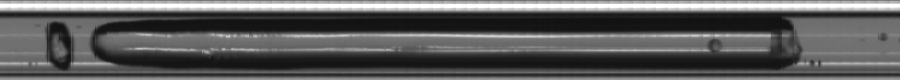
\includegraphics[width=\textwidth]{figuras/v8-panorama-plug}
  \caption{Trecho inicial do panorama espacial reconstruído de um ensaio de \textit{plug}
           (primeiras 900 colunas, de um total de 5940). O eixo horizontal corresponde à posição
           ao longo do percurso do escoamento; bolhas alongadas discretas alternam-se com trechos
           de líquido mais uniformes.}
  \label{fig:res-panorama-plug}
  \fonte{Elaborado pelo autor.}
\end{figure}

\begin{figure}[htbp]
  \centering
  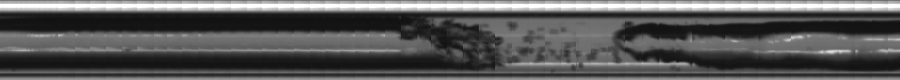
\includegraphics[width=\textwidth]{figuras/v8-panorama-slug}
  \caption{Trecho inicial do panorama espacial reconstruído de um ensaio de \textit{slug}
           (primeiras 900 colunas, de um total de 5071). As bolhas alongadas são mais longas e
           mais frequentes do que no \textit{plug}, mantido o fundo de líquido entre elas.}
  \label{fig:res-panorama-slug}
  \fonte{Elaborado pelo autor.}
\end{figure}

\begin{figure}[htbp]
  \centering
  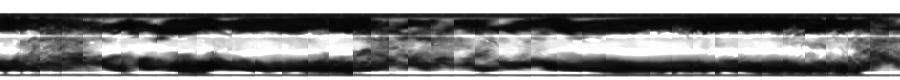
\includegraphics[width=\textwidth]{figuras/v8-panorama-churn}
  \caption{Trecho inicial do panorama espacial reconstruído de um ensaio de \textit{churn}
           (primeiras 900 colunas, de um total de 9586). A textura é densa e desorganizada, sem
           estruturas discretas bem definidas, refletindo o caráter agitado do regime.}
  \label{fig:res-panorama-churn}
  \fonte{Elaborado pelo autor.}
\end{figure}

\begin{figure}[htbp]
  \centering
  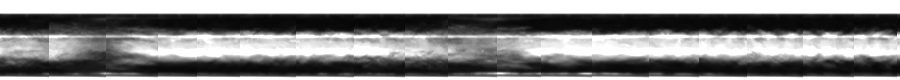
\includegraphics[width=\textwidth]{figuras/v8-panorama-annular}
  \caption{Trecho inicial do panorama espacial reconstruído de um ensaio de anular ondulado
           (primeiras 900 colunas, de um total de 23079). Um filme contínuo recobre a parede e a
           interface exibe uma ondulação fina e regular ao longo do percurso.}
  \label{fig:res-panorama-annular}
  \fonte{Elaborado pelo autor.}
\end{figure}

% =========================================================
\section{Sinais espaciais reconstruídos}\label{sec:res-sinais}
% =========================================================

Os sinais espaciais de brilho reconstruídos do panorama apresentaram-se como séries de milhares de
amostras por ensaio, com uma amostra por pixel de percurso do escoamento no tubo. Após a remoção de
tendência, da média e a normalização pelo desvio padrão, cada sinal ficou centrado em zero e com
variância unitária, expresso em unidades de desvio padrão. A \autoref{fig:res-sinais} mostra os
sinais de dois ensaios de \textit{churn}, sobrepostos no painel inferior. O brilho oscila ao longo
do eixo de percurso sem tendência residual, refletindo a passagem sucessiva das estruturas do
escoamento pela seção de visualização.

A mesma reconstrução foi obtida para os demais padrões, ilustrada nas
\autoref{fig:res-sinais-annular}, \autoref{fig:res-sinais-plug} e \autoref{fig:res-sinais-slug} para
anular ondulado, \textit{plug} e \textit{slug}, respectivamente. Os ensaios de \textit{plug} e de
\textit{slug} foram reconstruídos e analisados mesmo dispondo de poucos ensaios, quatro e três,
respectivamente, de modo que a sua inclusão tem caráter ilustrativo; essa limitação de amostragem é
retomada na discussão. Em
unidades de desvio padrão, os sinais crus dos quatro padrões têm aparência semelhante, uma oscilação
irregular em torno de zero, sem que a inspeção direta do sinal no tempo revele qual padrão o
originou. A característica que distingue os padrões não está na forma bruta do sinal, mas na
distribuição de energia por comprimento de onda, examinada no espectro de potência da
\autoref{sec:res-wps}.

\begin{figure}[htbp]
  \centering
  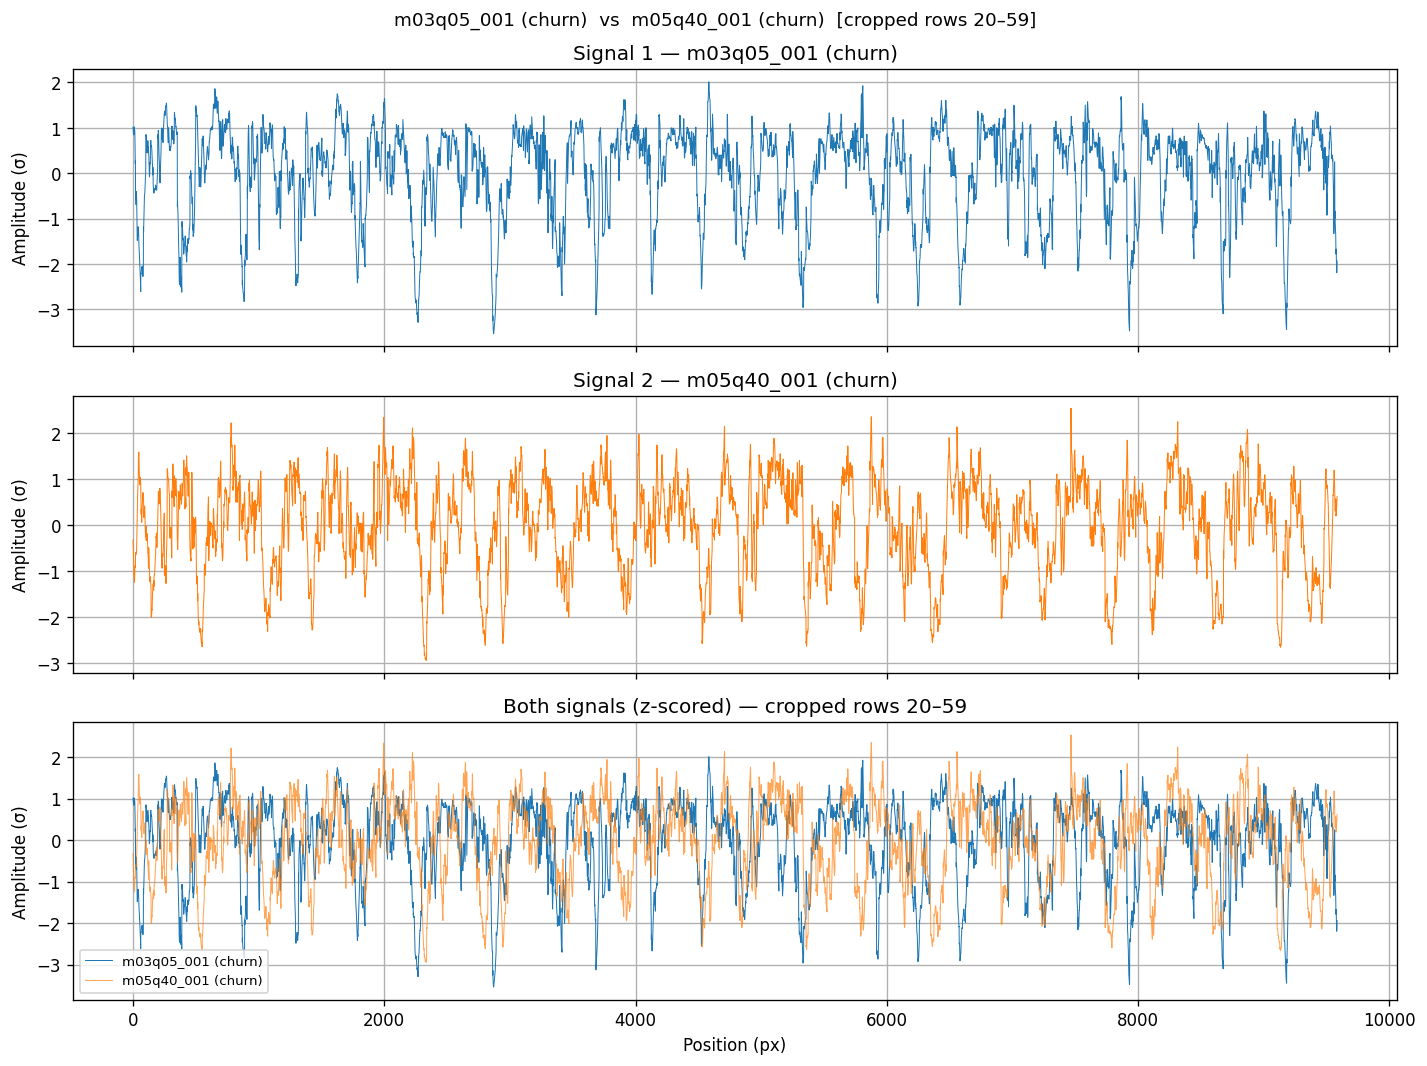
\includegraphics[width=0.92\textwidth]{figuras/v8-churn-churn-signals}
  \caption{Sinais espaciais de brilho de dois ensaios de \textit{churn}, na variante
           \textit{cropped} (média das linhas 20 a 59 do panorama), após pré-processamento.
           Painéis superior e central: cada ensaio isoladamente. Painel inferior: os dois sinais
           sobrepostos, em unidades de desvio padrão, ao longo da posição em pixels.}
  \label{fig:res-sinais}
  \fonte{Elaborado pelo autor.}
\end{figure}

\begin{figure}[htbp]
  \centering
  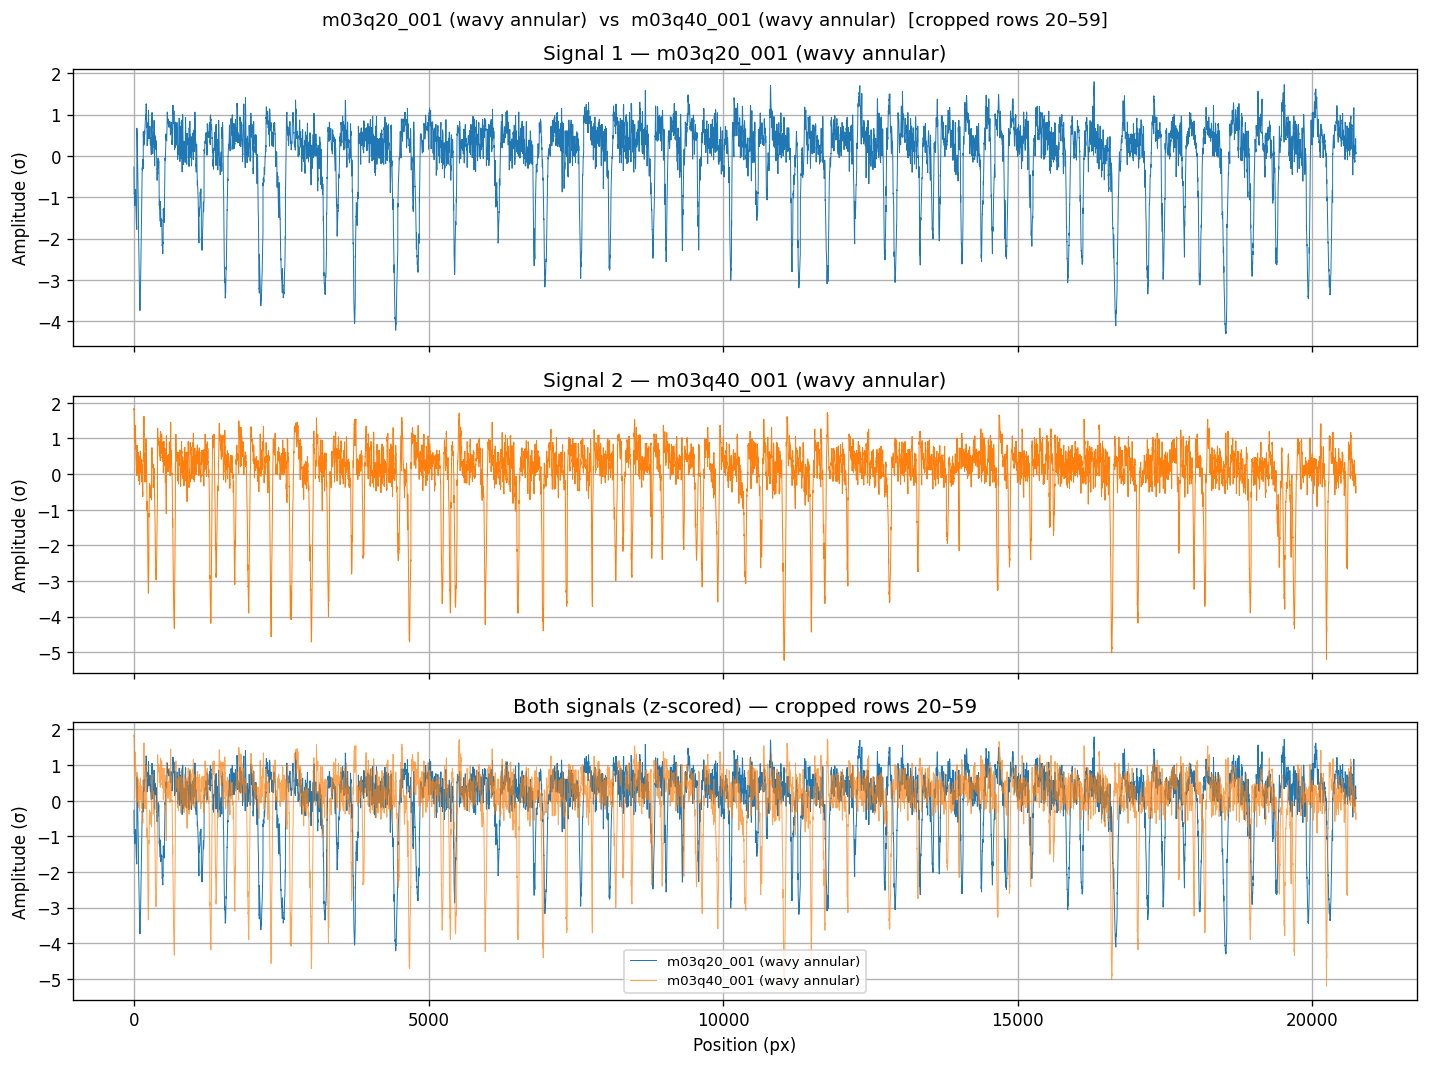
\includegraphics[width=0.92\textwidth]{figuras/v8-annular-signals}
  \caption{Sinais espaciais de brilho de dois ensaios de anular ondulado, na variante
           \textit{cropped}. Mesma disposição de painéis da \autoref{fig:res-sinais}.}
  \label{fig:res-sinais-annular}
  \fonte{Elaborado pelo autor.}
\end{figure}

\begin{figure}[htbp]
  \centering
  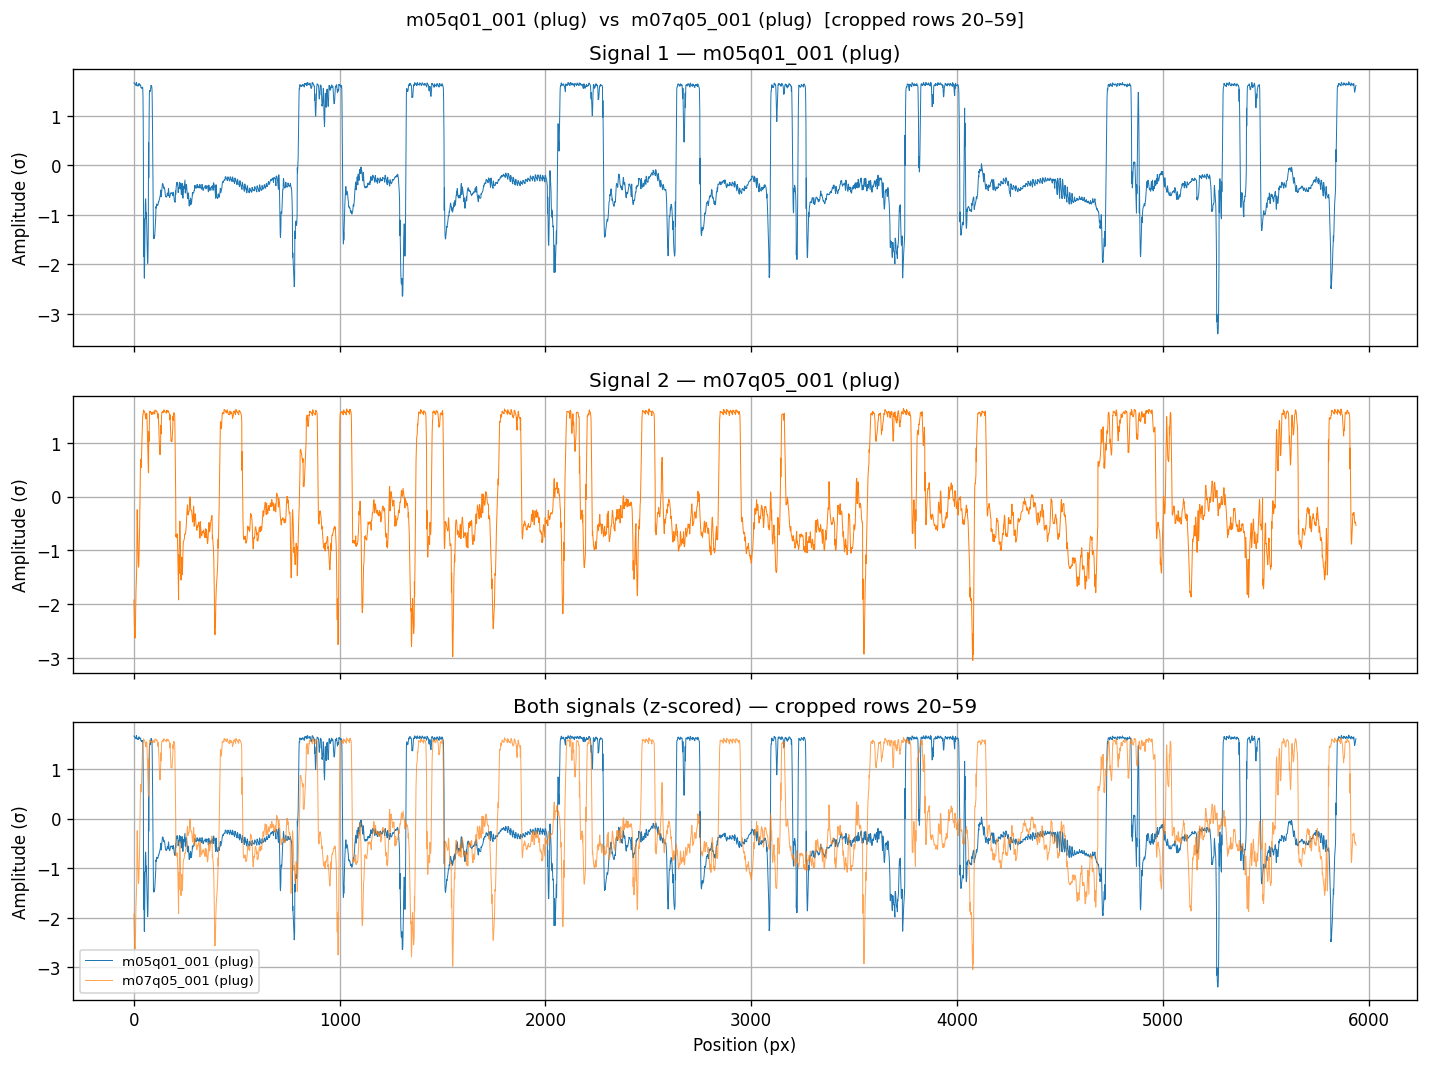
\includegraphics[width=0.92\textwidth]{figuras/v8-plug-signals}
  \caption{Sinais espaciais de brilho de dois ensaios de \textit{plug}, na variante
           \textit{cropped}. Mesma disposição de painéis da \autoref{fig:res-sinais}.}
  \label{fig:res-sinais-plug}
  \fonte{Elaborado pelo autor.}
\end{figure}

\begin{figure}[htbp]
  \centering
  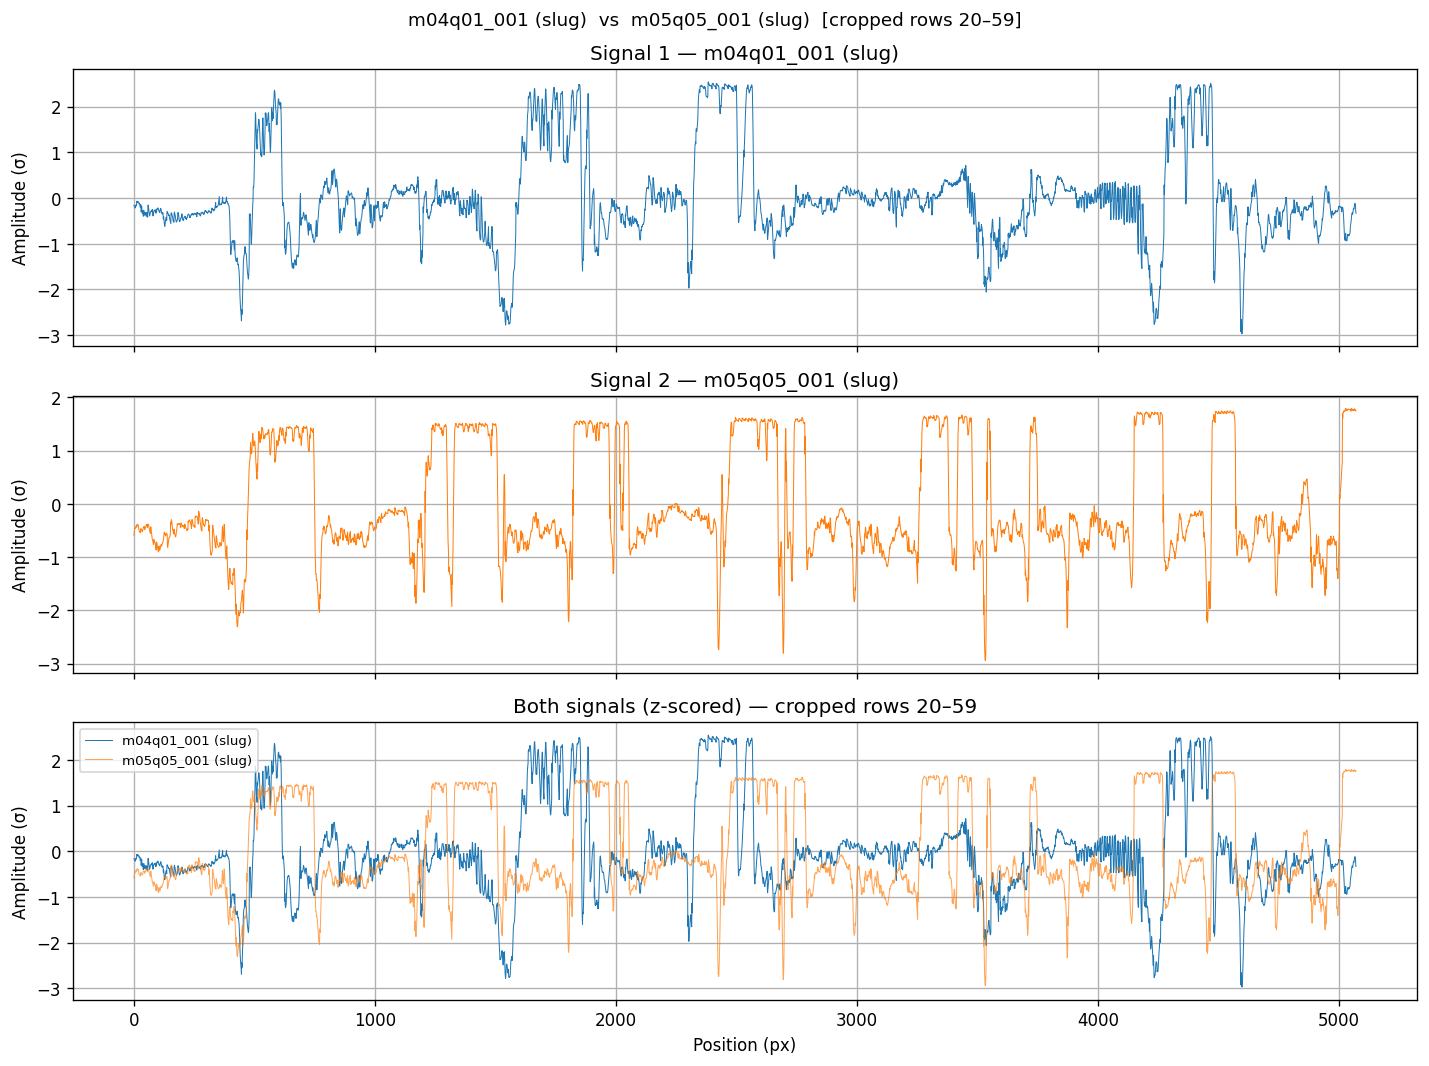
\includegraphics[width=0.92\textwidth]{figuras/v8-slug-signals}
  \caption{Sinais espaciais de brilho de dois ensaios de \textit{slug}, na variante
           \textit{cropped}. Mesma disposição de painéis da \autoref{fig:res-sinais}.}
  \label{fig:res-sinais-slug}
  \fonte{Elaborado pelo autor.}
\end{figure}

% =========================================================
\section{Espectro de potência e perfil de potência média}\label{sec:res-wps}
% =========================================================

Os campos de espectro de potência $\widetilde{P}_x(a)$ e $\widetilde{P}_y(a)$, obtidos da CWT das
funções de autocorrelação de cada ensaio, concentraram sua energia em uma faixa de comprimento de
onda bem delimitada. Em termos simples, a \textit{autocorrelação} mede o quanto o sinal de um
ensaio se parece consigo mesmo quando deslocado ao longo do percurso, revelando os tamanhos de
estrutura (comprimentos de onda) que se repetem no escoamento. A formulação de
\citeonline{schuck2019} parte dessas funções de correlação, e não do sinal bruto. O
\textit{espectro de potência} resultante indica quanta energia o padrão concentra em cada tamanho
de estrutura, e o \textit{perfil de potência média} $|\text{WPS}|$ resume essa informação em uma
única curva, cujo máximo aponta o comprimento de onda dominante do padrão. Nos ensaios de
\textit{churn} e de anular ondulado, essa concentração situou-se
na região de centenas de pixels de comprimento de onda, com o perfil de potência média
$|\text{WPS}|$ exibindo um máximo pronunciado nessa faixa e caindo para os comprimentos de onda mais
curtos e mais longos. Os painéis superiores da \autoref{fig:res-wps} mostram esse comportamento para
dois ensaios de \textit{churn}: os campos WPS apresentam um lóbulo central de magnitude elevada em
torno do atraso nulo, e os perfis de potência média ao lado exibem o pico correspondente na mesma
faixa de comprimento de onda.

\begin{figure}[htbp]
  \centering
  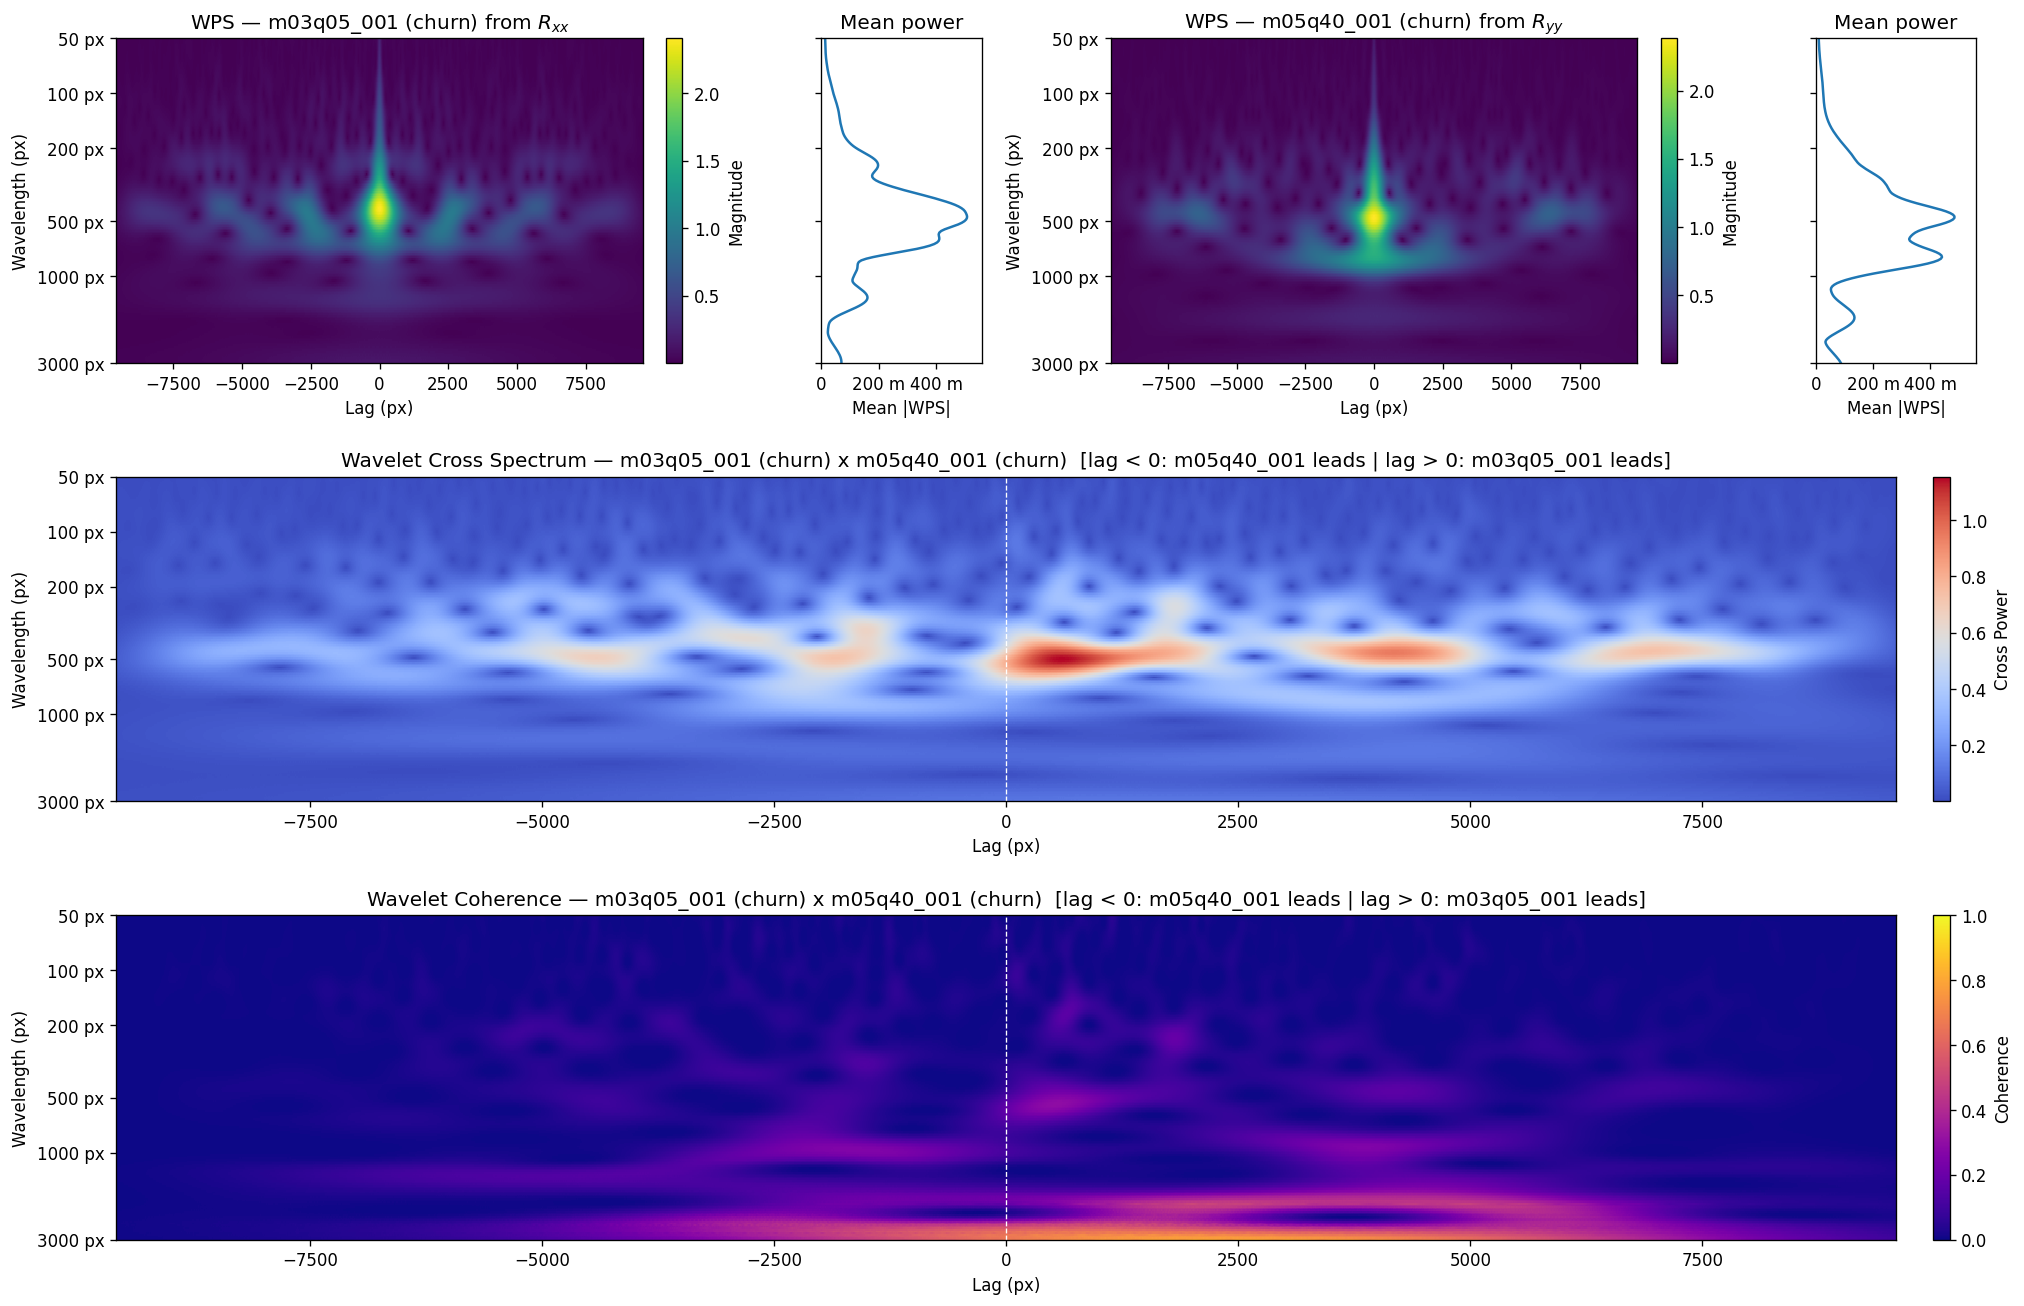
\includegraphics[width=\textwidth]{figuras/v8-churn-churn-wavelet}
  \caption{Campos espectrais de um par de ensaios de \textit{churn} (variante \textit{cropped}).
           Linha superior: espectro de potência $\widetilde{P}_x$ e $\widetilde{P}_y$ de cada
           ensaio, com o respectivo perfil de potência média $|\text{WPS}|$ ao lado. Linha central:
           espectro cruzado $\widetilde{C}_{xy}$. Linha inferior: coerência
           $\widetilde{\gamma}_{xy}$. Eixo vertical em comprimento de onda (pixels), eixo horizontal
           em atraso (pixels).}
  \label{fig:res-wps}
  \fonte{Elaborado pelo autor.}
\end{figure}

Essa faixa dominante mostrou-se a característica mais estável dos campos obtidos. O perfil de
potência média resumiu em uma única curva o comprimento de onda em que a energia espectral de cada
ensaio se concentra, e foi essa curva que apresentou o comportamento mais regular e mais fácil de
comparar entre ensaios, tanto na inspeção intra-padrão quanto na inter-padrão descritas adiante.

Para cada ensaio elegível, extraiu-se o comprimento de onda dominante $\lambda^*$, definido na
\autoref{sec:met-analise} como a posição do máximo do perfil de potência média $|\text{WPS}|$
na variante \textit{cropped}. O \autoref{quad:res-lambda} reúne a faixa de $\lambda^*$ observada em
cada padrão. Os ensaios de anular ondulado concentraram o máximo de potência na faixa mais estreita,
entre cerca de 350 e 570 pixels (mediana em torno de 490 pixels), ao passo que os de \textit{churn}
mantiveram o máximo majoritariamente entre cerca de 430 e 790 pixels (mediana em torno de 630
pixels), com um ensaio isolado deslocado para comprimentos de onda mais longos. Os padrões com
poucos ensaios apresentaram dispersão maior: \textit{plug} espalhou-se entre cerca de 220 e 710
pixels, enquanto \textit{slug} e \textit{slug}--\textit{churn} espalharam-se por uma faixa ampla,
chegando ao limite superior da grade de comprimentos de onda em um dos ensaios, o que reflete o
número reduzido de amostras desses padrões.

\begin{quadro}[htb]
  \centering
  \caption{Comprimento de onda dominante $\lambda^*$ (máximo do perfil de potência média
           $|\text{WPS}|$) por padrão, na variante \textit{cropped}, para os ensaios elegíveis
           de cada padrão. A coluna ``Coerência'' resume a leitura qualitativa da coerência no
           atraso nulo.}
  \label{quad:res-lambda}
  \begin{tabular}{l c c c c}
    \hline
    \textbf{Padrão} & \textbf{Ensaios} & \textbf{Faixa de $\lambda^*$ (px)} & \textbf{Mediana (px)} & \textbf{Coerência} \\
    \hline
    \textit{Churn}                      & 10 & 434--1264 & 629 & baixa/irregular \\
    Anular ondulado                     &  9 & 353--567  & 491 & baixa/irregular \\
    \textit{Plug}                       &  4 & 220--711  & 550 & baixa/irregular \\
    \textit{Slug}                       &  3 & 682--1213 & 711 & baixa/irregular \\
    \textit{Slug}--\textit{churn}       &  2 & 910--3000 & --- & baixa/irregular \\
    \hline
  \end{tabular}
  \fonte{Elaborado pelo autor.}
\end{quadro}

Os demais padrões apresentaram o mesmo arranjo de campos, deslocando apenas a posição da faixa
dominante. A \autoref{fig:res-wps-annular} mostra o par de anular ondulado, cujo perfil de potência
média concentra o máximo na faixa mais estreita e mais curta entre os padrões, em torno de 490
pixels. A \autoref{fig:res-wps-plug} e a \autoref{fig:res-wps-slug} mostram os pares de \textit{plug}
e de \textit{slug}, com o máximo mais disperso e deslocado para comprimentos de onda mais longos,
coerente com o número reduzido de ensaios registrado no \autoref{quad:res-lambda}. Em todos os casos,
a linha inferior de coerência permaneceu escura na maior parte da faixa, sem uma banda que
acompanhasse o máximo de potência, comportamento retomado na \autoref{sec:res-wco}.

\begin{figure}[htbp]
  \centering
  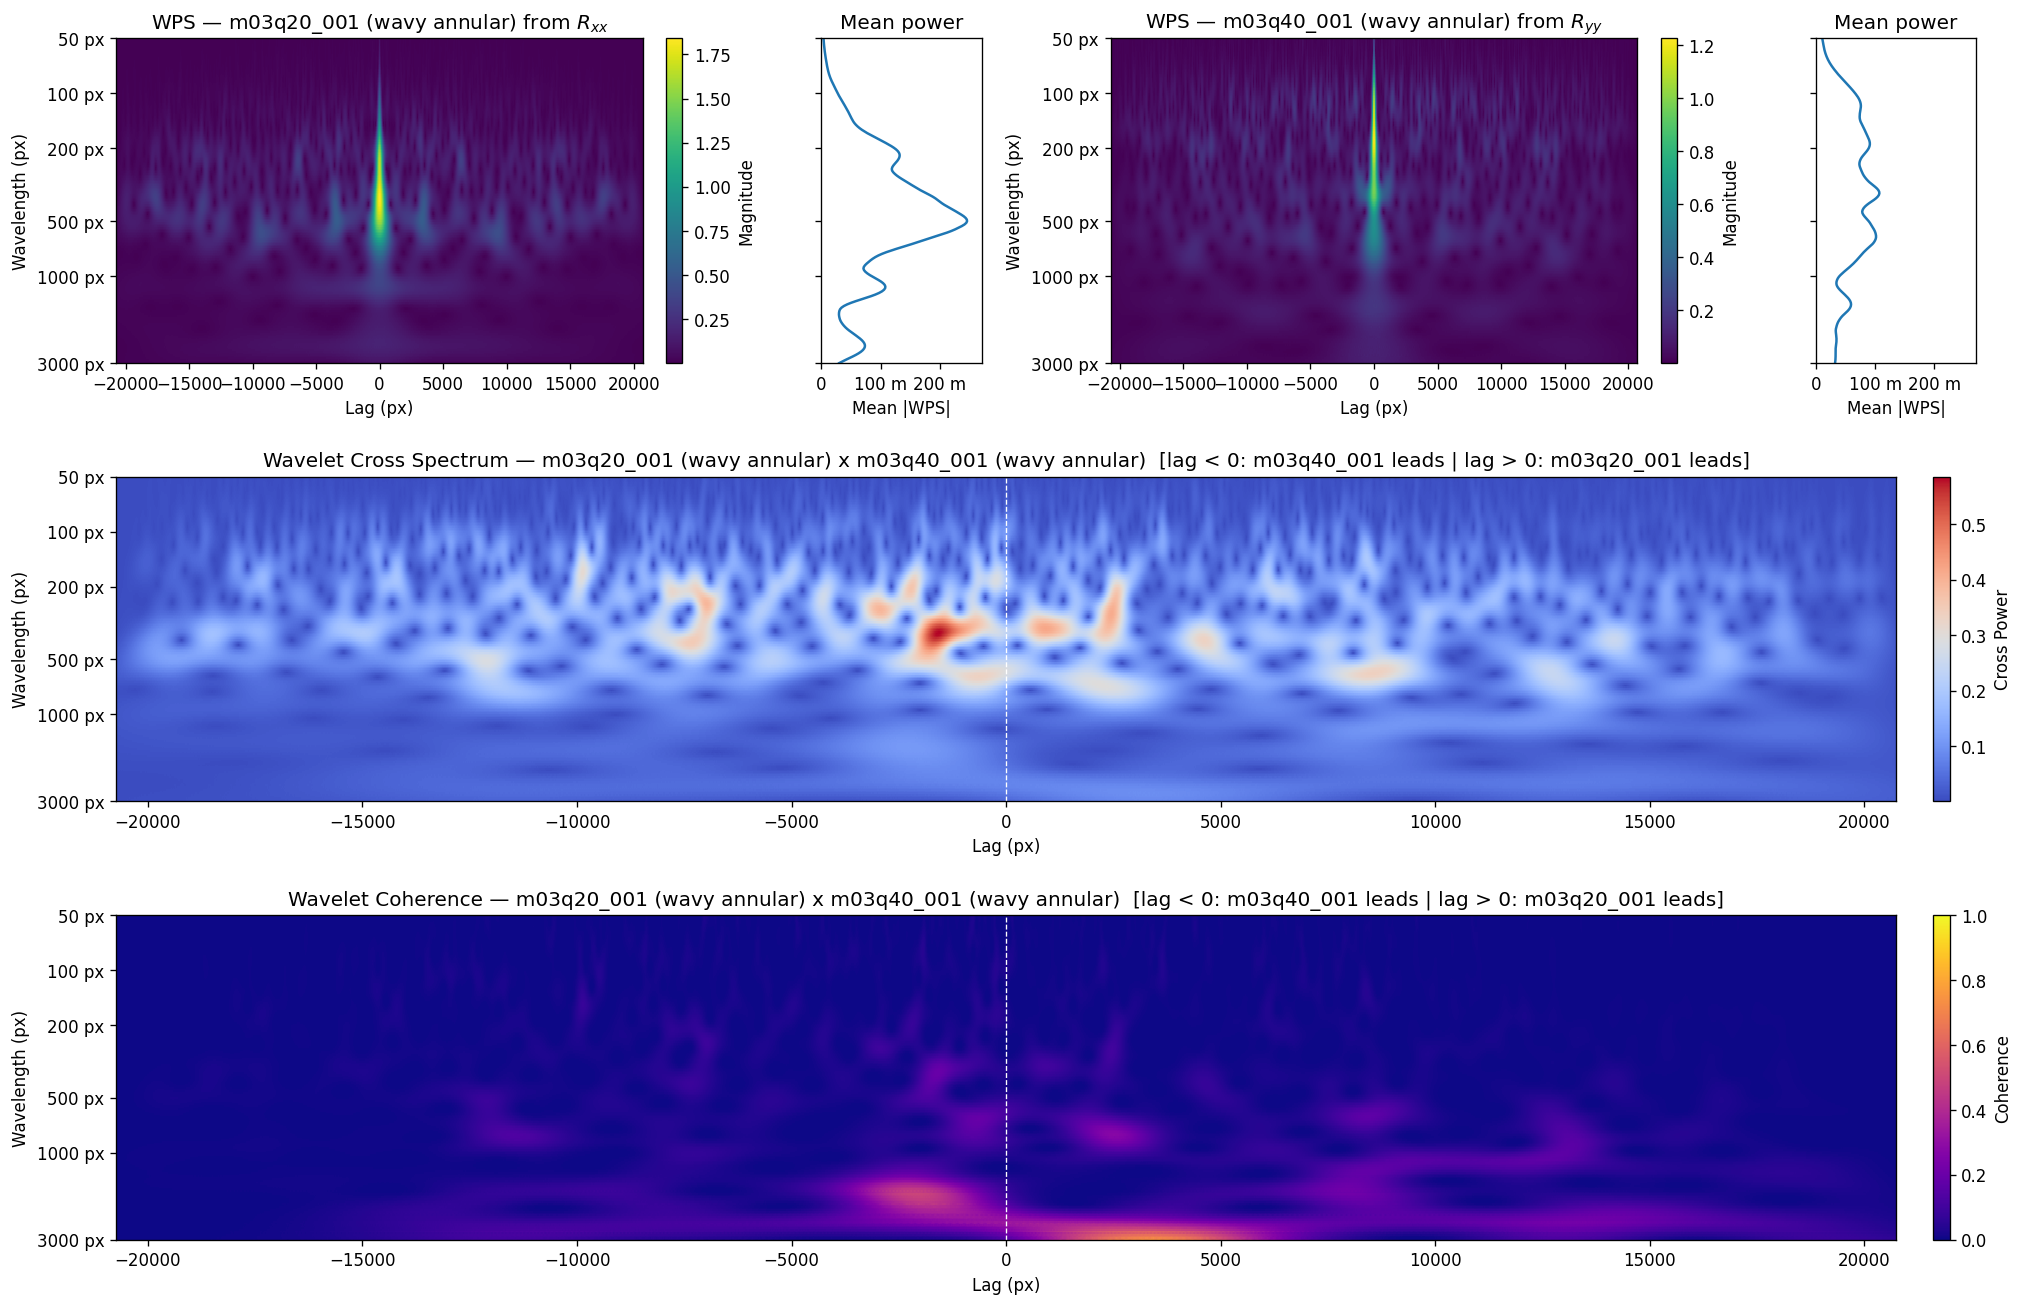
\includegraphics[width=\textwidth]{figuras/v8-annular-wavelet}
  \caption{Campos espectrais de um par de ensaios de anular ondulado (variante \textit{cropped}).
           Mesma disposição de painéis da \autoref{fig:res-wps}. O perfil de potência média
           concentra o máximo na faixa mais estreita e curta entre os padrões.}
  \label{fig:res-wps-annular}
  \fonte{Elaborado pelo autor.}
\end{figure}

\begin{figure}[htbp]
  \centering
  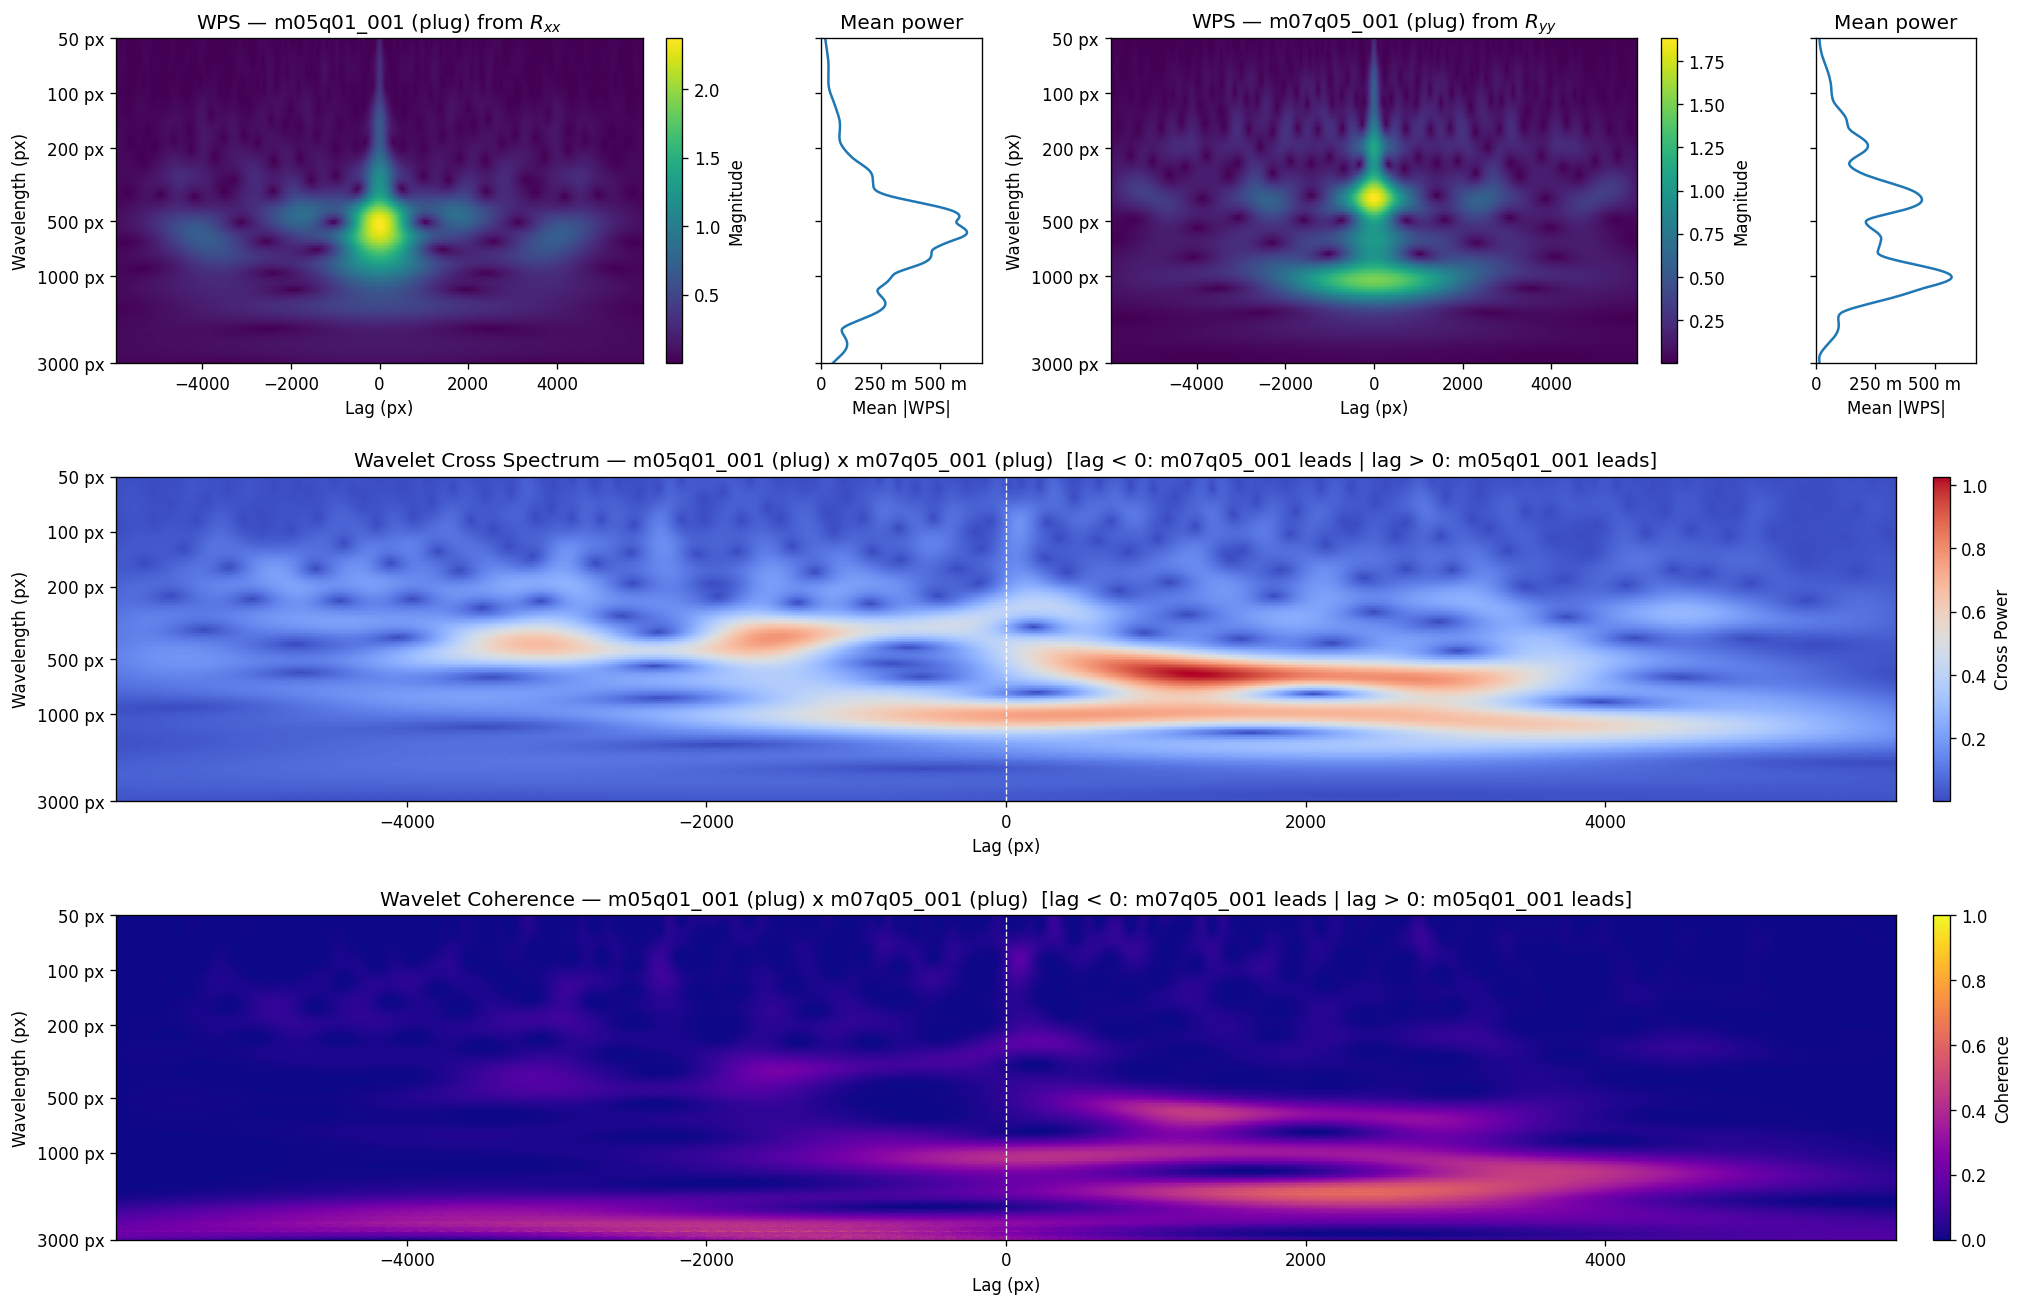
\includegraphics[width=\textwidth]{figuras/v8-plug-wavelet}
  \caption{Campos espectrais de um par de ensaios de \textit{plug} (variante \textit{cropped}).
           Mesma disposição de painéis da \autoref{fig:res-wps}.}
  \label{fig:res-wps-plug}
  \fonte{Elaborado pelo autor.}
\end{figure}

\begin{figure}[htbp]
  \centering
  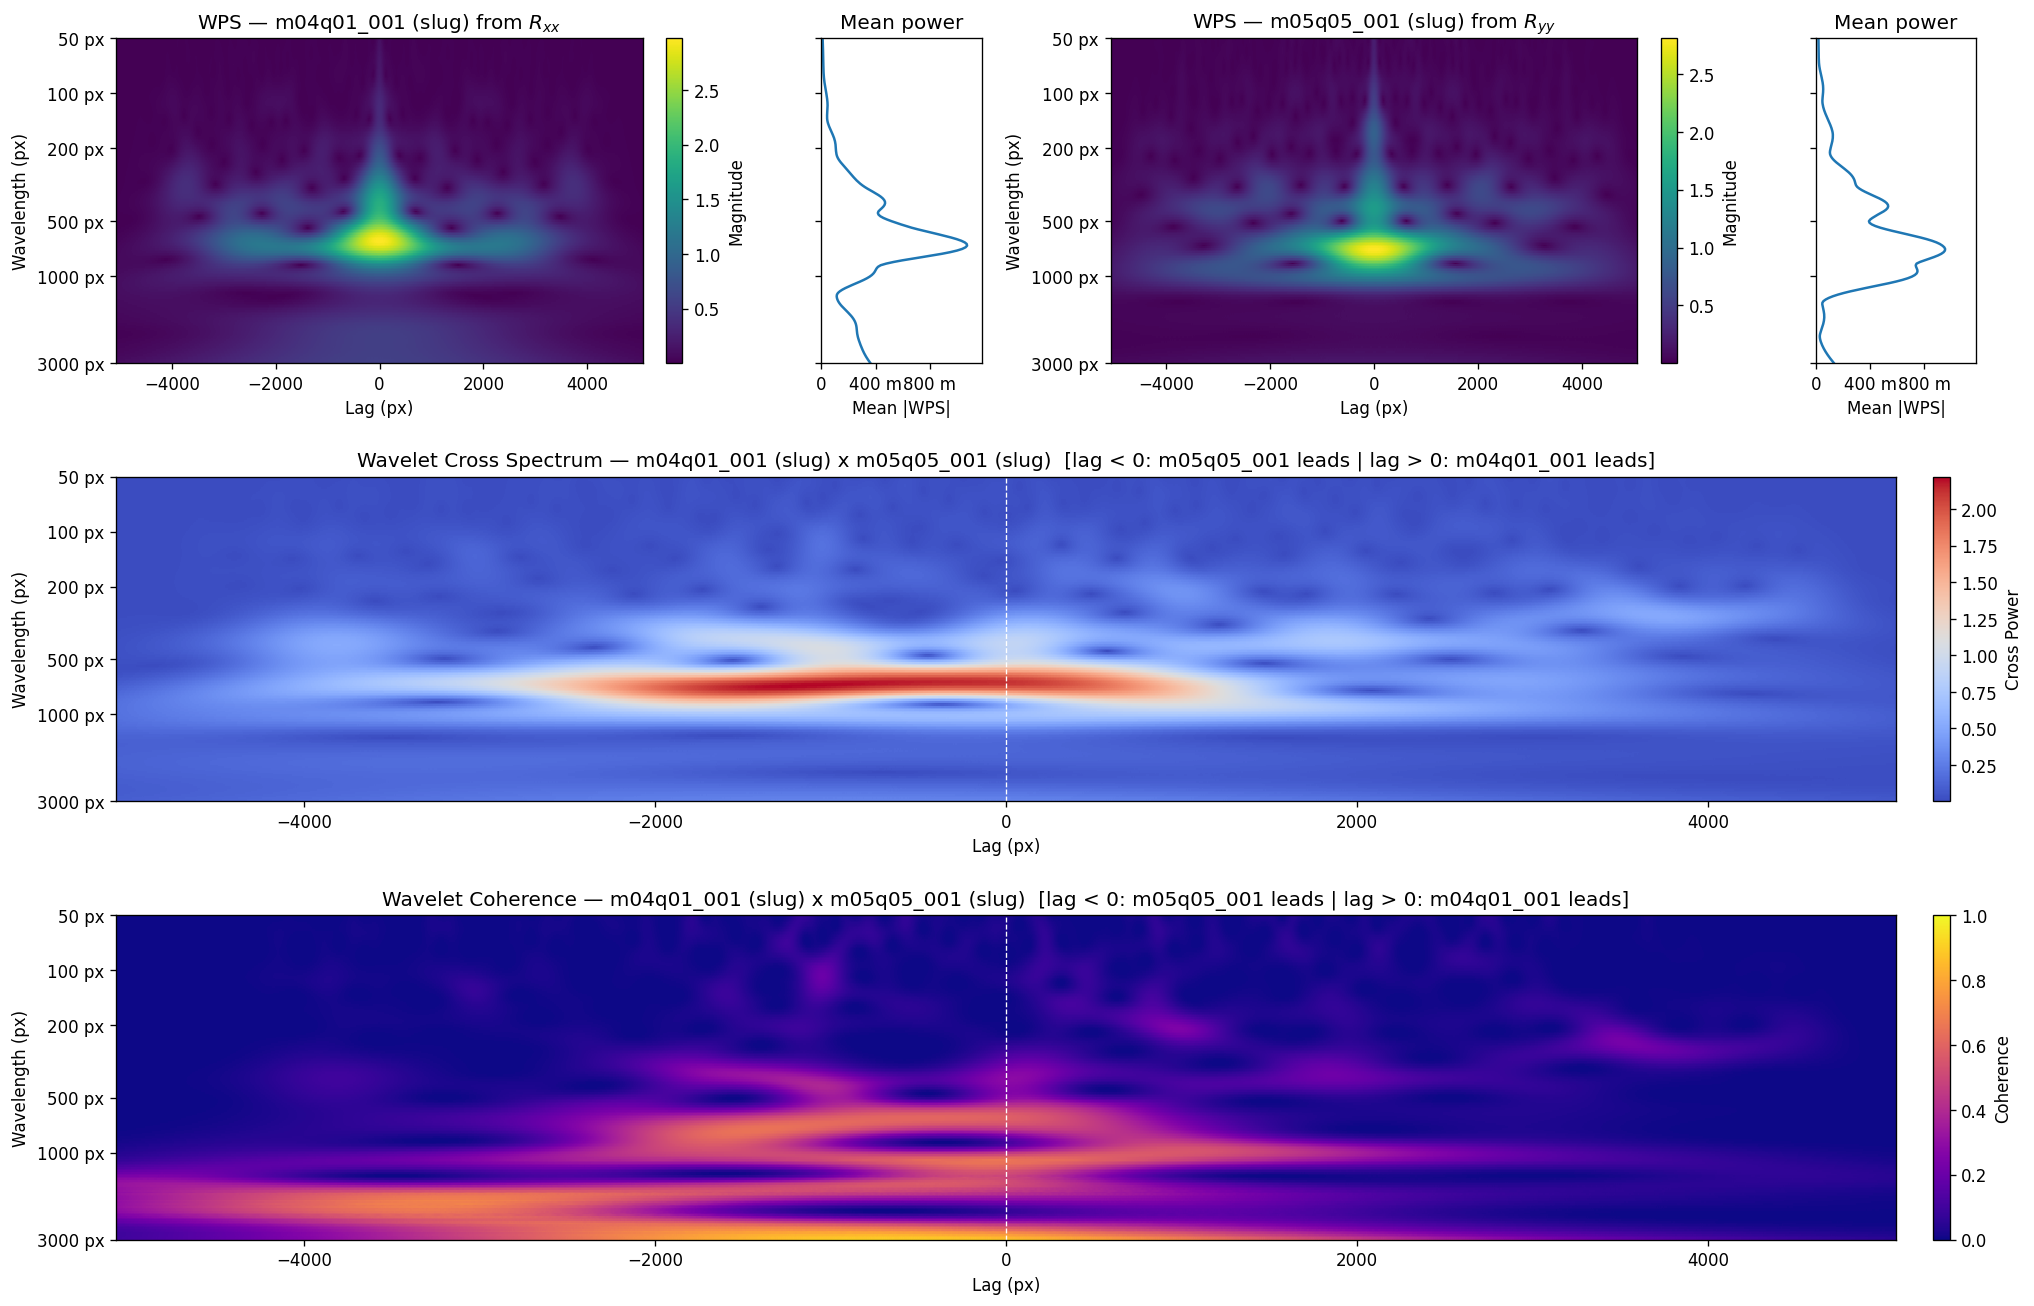
\includegraphics[width=\textwidth]{figuras/v8-slug-wavelet}
  \caption{Campos espectrais de um par de ensaios de \textit{slug} (variante \textit{cropped}).
           Mesma disposição de painéis da \autoref{fig:res-wps}.}
  \label{fig:res-wps-slug}
  \fonte{Elaborado pelo autor.}
\end{figure}

% =========================================================
\section{Campo de coerência \textit{Wavelet} alternativa}\label{sec:res-wco}
% =========================================================

O campo de coerência $\widetilde{\gamma}_{xy}(a)$, descritor principal deste trabalho, foi obtido
para todos os pares das duas campanhas. Antes de descrever o que se observou, convém explicar o
que cada campo representa. O \textit{espectro cruzado} (WCS) mede a energia que os dois ensaios
têm em comum em cada tamanho de estrutura. A \textit{coerência} (WCO), derivada dele, varia de
zero a um e indica o quanto os dois ensaios ``andam juntos'' em cada comprimento de onda, no
atraso nulo. A expectativa era de que dois ensaios de um mesmo padrão, por compartilharem o mesmo
tipo de estrutura, apresentassem coerência elevada na faixa dominante. Na inspeção dos campos, a
coerência avaliada no atraso nulo
apresentou-se em geral baixa e irregular ao longo dos comprimentos de onda, mesmo entre ensaios de
um mesmo padrão. Os valores de coerência mais altos concentraram-se nos comprimentos de onda
mais longos, nos quais a largura finita do campo abrange poucos períodos espaciais e a coerência
fica mal determinada. Por isso, a coerência elevada observada nessa região de ondas longas não
constitui evidência de acoplamento entre os ensaios. A linha inferior da \autoref{fig:res-wps} ilustra esse comportamento para o par de
ensaios de \textit{churn}: o campo de coerência permanece escuro na maior parte da faixa de
comprimentos de onda em torno do atraso nulo, sem uma banda de coerência elevada que acompanhe a
faixa dominante identificada nos perfis de potência média.

Esse resultado indica que a coerência \textit{Wavelet} alternativa, tomada no atraso nulo entre
pares de ensaios, não descreveu os padrões de escoamento com a precisão esperada para o arranjo e os
sinais utilizados. A caracterização mais consistente veio do perfil de potência média
$|\text{WPS}|$, cujo comportamento é retomado nas comparações a seguir.

% =========================================================
\section{Repetibilidade intra-padrão}\label{sec:res-intra}
% =========================================================

Na campanha intra-padrão, os campos de vários pares de ensaios de um mesmo padrão foram comparados
entre si. Os perfis de potência média $|\text{WPS}|$ dos ensaios de anular ondulado apresentaram o
comprimento de onda dominante na faixa mais concentrada entre os padrões, conforme o
\autoref{quad:res-lambda}, indicando que a posição do máximo de potência é a característica mais
reprodutível desse padrão. Os ensaios de \textit{churn} mantiveram o máximo na mesma ordem de
grandeza de um ensaio para outro, porém com dispersão maior, incluindo um ensaio com o máximo
deslocado para comprimentos de onda mais longos. Em ambos os padrões, a posição do máximo de potência
repetiu-se de forma mais evidente do que qualquer característica do campo de coerência. Os padrões
com menos ensaios (\textit{plug}, \textit{slug} e \textit{slug}--\textit{churn}) foram examinados de
forma ilustrativa, por disporem de poucos pares, e exibiram dispersão ainda maior do comprimento de
onda dominante, conforme os campos das \autoref{fig:res-wps-plug} e \autoref{fig:res-wps-slug}.

O campo de coerência $\widetilde{\gamma}_{xy}(a)$, por sua vez, não reproduziu essa regularidade:
entre pares de ensaios de um mesmo padrão a coerência no atraso nulo permaneceu baixa e sem uma banda
estável, de modo que a repetibilidade intra-padrão ficou muito mais evidente no perfil de potência
média do que no campo de coerência.

% =========================================================
\section{Separação inter-padrão}\label{sec:res-inter}
% =========================================================

Na campanha inter-padrão, os campos de pares de ensaios de padrões distintos foram comparados para
verificar se as assinaturas espectrais se distinguem de um padrão para outro. A
\autoref{fig:res-inter} mostra um par formado por um ensaio de \textit{churn} e um de anular
ondulado. Os perfis de potência média dos dois ensaios apresentaram faixas dominantes parcialmente
sobrepostas, na mesma ordem de comprimento de onda, de modo que a separação entre os dois padrões
por esse descritor mostrou-se sutil. Essa sobreposição é coerente com as faixas de comprimento de
onda dominante do \autoref{quad:res-lambda}: a faixa do anular ondulado está contida na faixa mais
ampla do \textit{churn}, de modo que o comprimento de onda dominante, isoladamente, não separa os
dois padrões, apenas desloca a mediana de um em relação ao outro. Os ensaios intermitentes de
\textit{plug} e de \textit{slug}, examinados de forma ilustrativa por disporem de poucos ensaios,
situam o comprimento de onda dominante em valores em geral mais longos e mais dispersos do que os
de anular ondulado, coerente com estruturas maiores e mais espaçadas; essa leitura, porém, apoia-se
em um número reduzido de ensaios e não sustenta uma separação inter-padrão firme. O campo de
coerência no atraso nulo, novamente baixo e irregular, não forneceu uma distinção nítida entre os
padrões.

\begin{figure}[htbp]
  \centering
  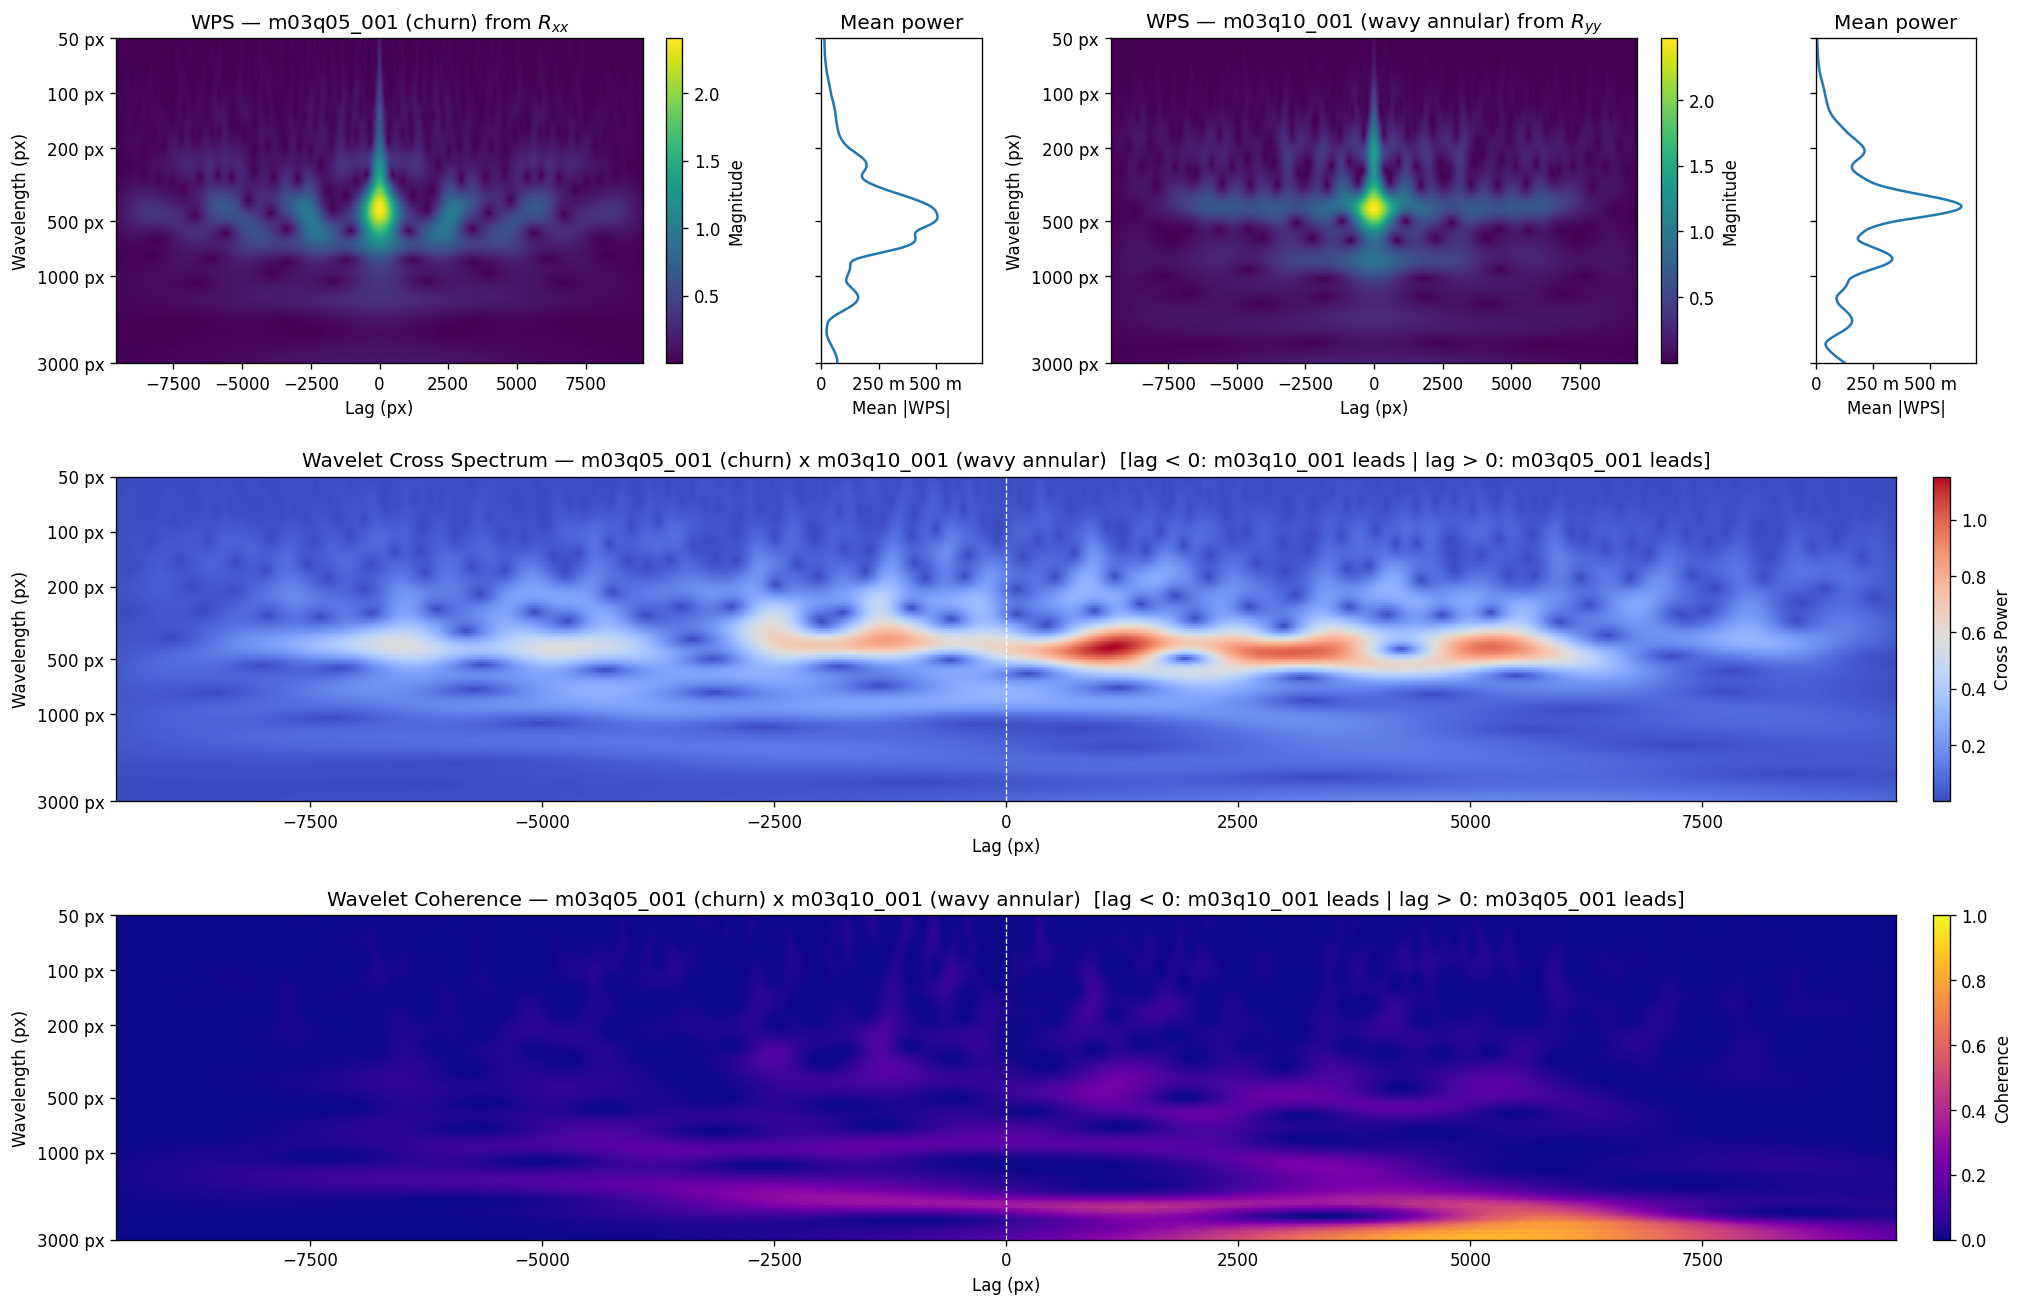
\includegraphics[width=\textwidth]{figuras/v8_1-churn-annular-wavelet}
  \caption{Campos espectrais de um par inter-padrão, um ensaio de \textit{churn} e um de anular
           ondulado (variante \textit{cropped}). Mesma disposição de painéis da
           \autoref{fig:res-wps}. Os perfis de potência média apresentam faixas dominantes
           parcialmente sobrepostas entre os dois padrões.}
  \label{fig:res-inter}
  \fonte{Elaborado pelo autor.}
\end{figure}

As combinações entre padrões foram inspecionadas de forma sistemática, abrangendo os duzentos e
oitenta e sete pares formados pelo produto dos ensaios de cada par de padrões (\textit{churn},
anular ondulado, \textit{plug}, \textit{slug} e \textit{slug}--\textit{churn}). O comportamento
ilustrado na \autoref{fig:res-inter} repetiu-se nas demais combinações: a coerência no atraso nulo
manteve-se baixa e irregular, sem distinção nítida entre padrões, e as faixas dominantes de
$\lambda^*$ apresentaram apenas sobreposição parcial. Cada par foi registrado como figura no
conjunto de resultados, o que assegura a rastreabilidade da inspeção visual, embora não se tenham
extraído descritores numéricos por par.

A quantificação da separação entre padrões em nível de ensaio é apresentada na
\autoref{sec:res-limite-estat}, em que a matriz de distância espectral e o teste ANOSIM fornecem a
evidência estatística correspondente. Ela abrange os quatro padrões com mais de dois ensaios
(\textit{churn}, anular ondulado, \textit{plug} e \textit{slug}); o \textit{slug}--\textit{churn},
com apenas dois ensaios, permaneceu de caráter ilustrativo.

% =========================================================
\section{Quantificação estatística da repetibilidade}\label{sec:res-limite-estat}
% =========================================================

A leitura qualitativa dos campos foi complementada por uma quantificação estatística da
repetibilidade do descritor espectral, destinada a medir objetivamente o quanto ensaios de um mesmo
padrão de escoamento se parecem entre si em comparação com ensaios de padrões diferentes. Essa
quantificação confirma e dimensiona o que a inspeção visual já indicava: a semelhança intra-padrão
existe, mas é sutil --- não uma distinção evidente, como a que separa duas classes de objetos
claramente distintas, e sim uma semelhança modesta, do tipo que se percebe entre dois exemplares
aparentados, com um ``ar de família'' acompanhado de considerável variação dentro de cada grupo. A
análise abrangeu os quatro padrões com mais de dois ensaios, \textit{churn} (dez ensaios), anular
ondulado (nove), \textit{plug} (quatro) e \textit{slug} (três), totalizando vinte e seis ensaios; o
\textit{slug}--\textit{churn}, com apenas dois ensaios, ficou de fora por não sustentar uma leitura
de grupo. As subseções a seguir apresentam, de forma didática, o propósito de cada etapa, o
resultado esperado e o que de fato se obteve.

% ---------------------------------------------------------
\subsection{Métrica de distância espectral entre ensaios}\label{sec:res-estat-distancia}
% ---------------------------------------------------------

O descritor submetido à análise não foi o campo de coerência, mas o perfil de potência média
$|\text{WPS}|$ por ensaio, que foi a característica mais reprodutível identificada na inspeção dos
campos. Para cada ensaio tomou-se o perfil de potência média na coluna de atraso nulo, branqueado
por escala pela remoção do decaimento espectral comum de fundo, de modo que o descritor retenha a
\emph{forma} do espectro, isto é, em quais tamanhos de estrutura a energia se concentra, e não a sua
amplitude bruta. Para que todos os ensaios tenham o mesmo comprimento, as séries foram truncadas ao
tamanho do menor ensaio de \textit{churn}. Por essa razão, o descritor usado aqui difere do perfil
de potência média de sinal completo que originou o comprimento de onda dominante $\lambda^*$ do
\autoref{quad:res-lambda}, cujos valores não devem ser lidos como entrada direta do teste.

A semelhança entre dois ensaios foi medida pela \emph{correlação de Pearson} entre seus perfis: um
número que resume o quanto duas curvas sobem e descem juntas, próximo de um quando têm a mesma forma
e próximo de zero quando não guardam relação. A partir dela define-se a \emph{distância} entre dois
ensaios $i$ e $j$ como um menos essa correlação,

\begin{equation}\label{eq:dist-pearson}
  d_{ij} = 1 - \rho(\mathbf{z}_i, \mathbf{z}_j),
\end{equation}

\noindent em que $\mathbf{z}_i$ e $\mathbf{z}_j$ são os perfis de potência branqueados dos dois
ensaios e $\rho$ é a correlação de Pearson entre eles. Em termos do cálculo, $\rho$ compara os dois
perfis frequência a frequência: para cada frequência verifica se os dois ensaios estão
simultaneamente acima ou abaixo da sua própria energia média e, somando essas concordâncias ao longo
de todo o espectro, resume em um único número se as duas curvas sobem e descem em sintonia. Vale
próximo de um quando os perfis têm picos e vales nas mesmas frequências (mesma forma espectral), em
torno de zero quando não há relação entre eles e torna-se negativo quando têm formas opostas --- um
com pico onde o outro tem vale ---, caso em que a distância da \autoref{eq:dist-pearson} ultrapassa a
unidade. Por depender apenas da forma relativa das curvas, e não de sua amplitude bruta, $\rho$ é
insensível à escala de energia de cada ensaio. Assim, ensaios de forma idêntica têm distância
nula e ensaios sem relação têm distância próxima de um. Calculando essa distância para todos os pares
obtém-se uma matriz de distâncias entre os vinte e seis ensaios, representada no
\autoref{fig:res-dmatrix}. Nela, os blocos na diagonal reúnem os ensaios de um mesmo padrão. A
predominância de tons mais claros (menor distância) nesses blocos, em relação aos blocos fora da
diagonal, é a manifestação visual da semelhança intra-padrão que a análise quantifica. Chama a
atenção um ensaio de \textit{plug} (o ensaio 21) cujas linha e coluna são escuras em quase toda a
extensão: sua assinatura espectral é atípica, anticorrelacionada com a da maioria dos demais
ensaios. Trata-se de variação real desse ensaio, mantida na análise e não removida, e explica em
parte por que o grupo \textit{plug} é internamente heterogêneo.

\begin{figure}[htbp]
  \centering
  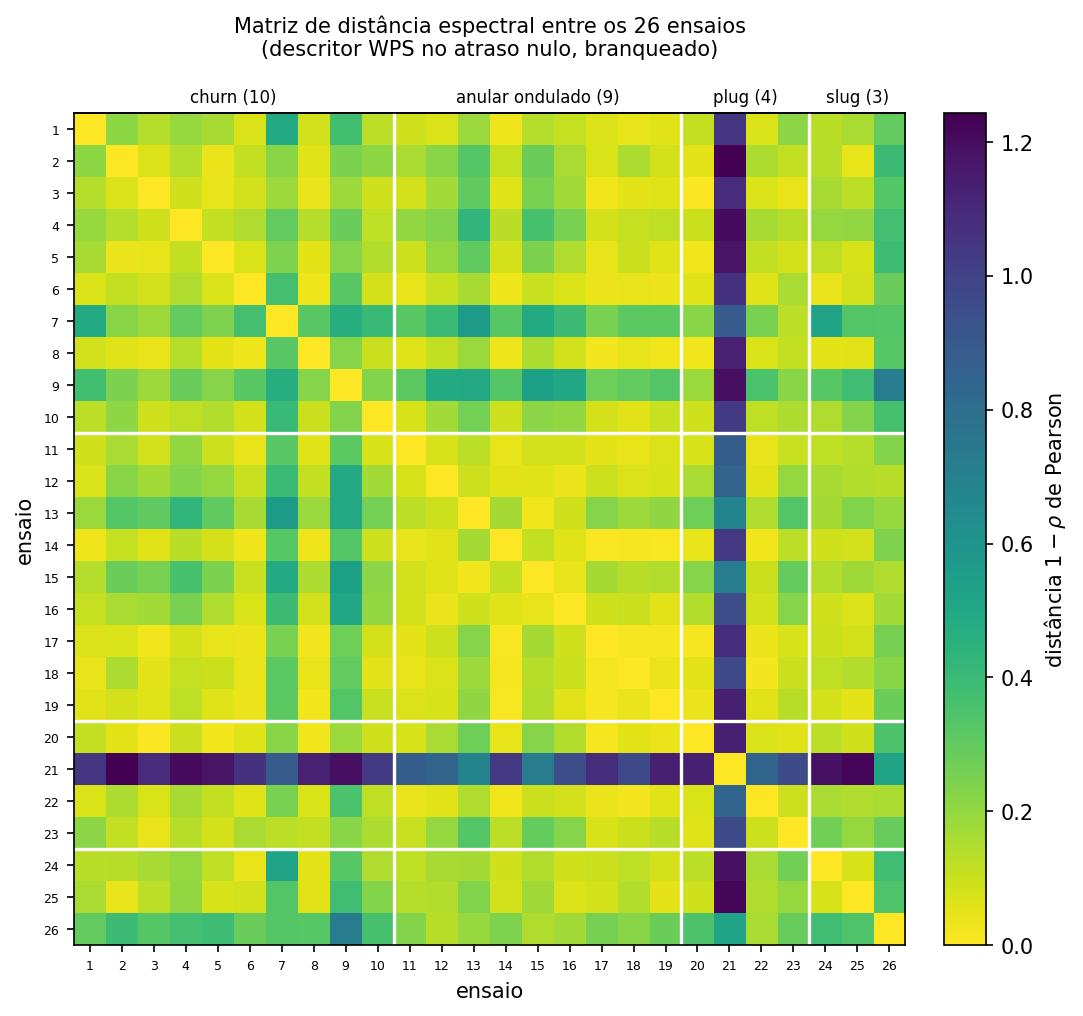
\includegraphics[width=0.78\textwidth]{figuras/v8-estat-dmatrix}
  \caption{Matriz de distância espectral ($1$ menos a correlação de Pearson entre os perfis de
           potência branqueados) entre os vinte e seis ensaios, ordenados por padrão
           (\textit{churn}, ensaios 1 a 10; anular ondulado, 11 a 19; \textit{plug}, 20 a 23;
           \textit{slug}, 24 a 26). Cores mais claras indicam ensaios mais parecidos; as linhas
           brancas separam os quatro padrões, e os blocos na diagonal correspondem a pares de um
           mesmo padrão. A cruz escura no ensaio 21 (um \textit{plug}) assinala um ensaio de
           assinatura atípica, anticorrelacionado com quase todos os demais.}
  \label{fig:res-dmatrix}
  \fonte{Elaborado pelo autor.}
\end{figure}

% ---------------------------------------------------------
\subsection{Teste de similaridade entre grupos (ANOSIM)}\label{sec:res-estat-anosim}
% ---------------------------------------------------------

Sobre a matriz de distâncias aplicou-se o coeficiente $R$ de ANOSIM, um teste simples de
comparação entre grupos. Ele ordena todas as $M = \binom{n}{2}$ distâncias da menor para a maior,
atribuindo a cada uma um posto, e compara o posto médio das distâncias ``mesmo padrão'' com o das
distâncias ``padrões diferentes'' por meio do coeficiente

\begin{equation}\label{eq:anosim-r}
  R = \frac{\bar{r}_{\text{entre}} - \bar{r}_{\text{dentro}}}{M/2},
\end{equation}

\noindent em que $\bar{r}_{\text{entre}}$ e $\bar{r}_{\text{dentro}}$ são os postos médios das
distâncias entre padrões distintos e dentro de um mesmo padrão, respectivamente, e $M = \binom{n}{2}$
é o número total de pares de distâncias entre os $n$ ensaios.

O cálculo dos dois postos médios parte de uma única ordenação e segue três passos:

\begin{enumerate}
  \item \textbf{Ranquear.} Todas as $M$ distâncias da matriz são ordenadas em conjunto, sem
        distinguir sua natureza: a menor recebe o posto $1$, a seguinte o posto $2$, e assim por
        diante até a maior, que recebe o posto $M$.
  \item \textbf{Rotular.} Cada par é então classificado conforme os ensaios que o compõem ---
        ``mesmo padrão'', quando ambos pertencem ao mesmo regime, ou ``padrões diferentes'', caso
        contrário.
  \item \textbf{Comparar.} Calcula-se a média dos \emph{postos} (não das distâncias) em cada grupo,
        obtendo $\bar{r}_{\text{dentro}}$ e $\bar{r}_{\text{entre}}$, e toma-se a diferença entre as
        duas.
\end{enumerate}

\noindent Por operar sobre postos, e não sobre os valores absolutos das distâncias, o coeficiente é
insensível à escala da métrica. A diferença $\bar{r}_{\text{entre}} - \bar{r}_{\text{dentro}}$ mede,
então, o quanto os pares de mesmo padrão se concentram entre as menores distâncias da matriz: se os
ensaios de um mesmo regime forem sistematicamente os mais próximos, esses pares ocupam os postos
baixos, $\bar{r}_{\text{dentro}}$ fica pequeno e a diferença torna-se positiva; se o rótulo não tiver
relação com a distância, os dois postos médios se igualam e a diferença se anula. O denominador
$M/2$ é apenas o fator que normaliza essa diferença para o intervalo $[-1, 1]$, correspondendo ao
valor máximo que o numerador pode assumir sob separação perfeita.

O coeficiente $R$ vale próximo de zero quando os dois grupos são indistinguíveis e próximo
de um quando os ensaios de um mesmo padrão são sistematicamente mais próximos entre si do que os de
padrões diferentes. Esperava-se um valor alto, caso os padrões se separassem bem pelo descritor
espectral. O valor observado, tomando os quatro padrões em conjunto, foi $R = 0{,}20$, indicando que
ensaios de um mesmo padrão são, em média, apenas \emph{modestamente} mais próximos entre si do que
ensaios de padrões distintos. Esse valor é coerente com o \autoref{fig:res-estat-ecdf}, que mostra as
distribuições acumuladas empíricas (ECDF) das distâncias intra-padrão e inter-padrão. A ECDF é a
curva que, para cada valor de distância no eixo horizontal, informa a fração de pares de ensaios
com distância menor ou igual a esse valor, de modo que a curva deslocada para a esquerda indica
distâncias sistematicamente menores. A curva intra-padrão situa-se de forma consistente à esquerda
da inter-padrão, com as distâncias de mesmo padrão sistematicamente menores, embora o deslocamento
entre as duas curvas seja pequeno.

\begin{figure}[htbp]
  \centering
  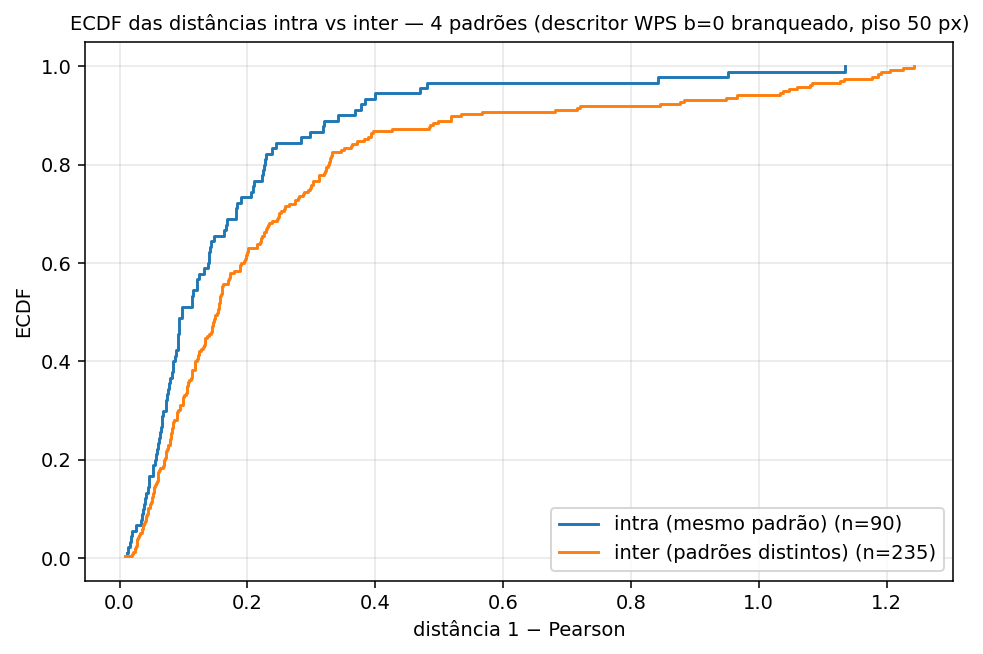
\includegraphics[width=0.82\textwidth]{figuras/v8-estat-ecdf}
  \caption{Distribuição acumulada (ECDF) das distâncias espectrais entre ensaios: dentro de um
           mesmo padrão (\textit{intra}, noventa pares) e entre padrões distintos (\textit{inter},
           duzentos e trinta e cinco pares). A curva intra-padrão, deslocada para a esquerda,
           traduz a separação sutil quantificada por $R = 0{,}20$.}
  \label{fig:res-estat-ecdf}
  \fonte{Elaborado pelo autor.}
\end{figure}

Com quatro padrões, um único coeficiente global esconde quais padrões de fato se separam. Por isso
calculou-se também o $R$ de ANOSIM para cada um dos seis pares de padrões, restringindo a matriz aos
dois grupos de cada vez. O \autoref{quad:res-anosim-pares} reúne esses valores. A leitura par-a-par
revela uma estrutura clara: o anular ondulado é o padrão mais distinto, separando-se bem de todos os
regimes mais lentos, com o maior $R$ de todos frente ao \textit{slug} ($0{,}52$) e separação clara
frente ao \textit{plug} ($0{,}32$). O \textit{slug} é o padrão intermitente que mais contrasta, tanto
com o anular quanto com o \textit{churn} ($0{,}22$). Em contrapartida, \textit{churn} e \textit{plug}
são praticamente indistinguíveis por este descritor ($R = 0{,}03$), e a separação entre \textit{churn}
e anular ondulado permanece fraca ($0{,}18$), reproduzindo o valor já observado quando apenas esses
dois padrões eram comparados. O par \textit{plug}--\textit{slug} ($0{,}11$) apoia-se em poucos pares
de ensaios e deve ser lido com cautela.

\begin{quadro}[htb]
  \centering
  \caption{Coeficiente $R$ de ANOSIM par-a-par entre os quatro padrões, calculado restringindo a
           matriz de distância aos dois grupos de cada par.}
  \label{quad:res-anosim-pares}
  \begin{tabular}{@{}p{0.40\textwidth} c c p{0.28\textwidth}@{}}
    \hline
    \textbf{Par de padrões} & \textbf{$R$} & \textbf{Pares} & \textbf{Leitura} \\
    \hline
    anular ondulado $\times$ \textit{slug}  & $0{,}52$ & 66  & separação mais forte \\
    anular ondulado $\times$ \textit{plug}  & $0{,}32$ & 78  & separação clara \\
    \textit{churn} $\times$ \textit{slug}   & $0{,}22$ & 78  & separação moderada \\
    \textit{churn} $\times$ anular ondulado & $0{,}18$ & 171 & fraca \\
    \textit{plug} $\times$ \textit{slug}    & $0{,}11$ & 21  & fraca, $n$ pequeno \\
    \textit{churn} $\times$ \textit{plug}   & $0{,}03$ & 91  & praticamente indistinguíveis \\
    \hline
  \end{tabular}
  \fonte{Elaborado pelo autor.}
\end{quadro}

% ---------------------------------------------------------
\subsection{Significância por teste de permutação}\label{sec:res-estat-permuta}
% ---------------------------------------------------------

Para avaliar se um $R$ dessa magnitude poderia surgir por acaso, construiu-se uma ``régua do
acaso'' por reamostragem: embaralham-se os rótulos de padrão entre os ensaios e recalcula-se $R$
para cada reatribuição, obtendo a distribuição de valores que o coeficiente assumiria se os rótulos
não guardassem relação com a semelhança espectral. Sob essas reatribuições aleatórias o coeficiente
distribui-se em torno de zero, com percentil noventa e cinco em torno de $0{,}18$, de modo que o
valor observado de $0{,}20$ situa-se logo acima dessa régua, indicando uma separação modesta, com
considerável sobreposição entre os grupos.

O embaralhamento, porém, não pode ser totalmente livre. Cada ensaio foi coletado sob uma combinação
de fluxo de calor e fluxo mássico, e essas condições acompanham o padrão na grade experimental. Se
os rótulos fossem embaralhados sem restrição, confundir-se-ia o efeito do padrão com o efeito da
condição de operação. Por isso as reatribuições foram permitidas apenas \emph{dentro} de estratos de
condição semelhante, controlando um fator operacional de cada vez --- uma estratificação por fluxo
de calor e, separadamente, uma por fluxo mássico. A estratificação por fluxo de calor é mal
condicionada, pois com quatro padrões vários de seus estratos ficam puros ou quase puros em padrão,
deixando pouco a permutar, e forneceu $p = 0{,}019$ apenas como linha de comparação. A estratificação
por fluxo mássico, melhor condicionada por misturar os quatro padrões em seus estratos centrais, é a
referência honesta e forneceu $p = 0{,}030$. Sem controle algum de condição, o valor seria $p =
0{,}017$. O \autoref{quad:res-anosim} reúne esses valores.

\begin{quadro}[htb]
  \centering
  \caption{Resumo do teste de repetibilidade (ANOSIM sobre a matriz de distância espectral, quatro
           padrões).}
  \label{quad:res-anosim}
  \begin{tabular}{@{}p{0.46\textwidth} c p{0.34\textwidth}@{}}
    \hline
    \textbf{Grandeza} & \textbf{Valor} & \textbf{Leitura} \\
    \hline
    $R$ de ANOSIM global (observado)            & $0{,}20$  & separação fraca a moderada, porém real \\
    $p$ — estrat. por fluxo mássico             & $0{,}030$ & bem condicionado, referência \\
    $p$ — estrat. por fluxo de calor            & $0{,}019$ & mal condicionado (estratos puros) \\
    $p$ — sem estratificação                    & $0{,}017$ & contexto, sem controle de confusão \\
    percentil 95 de $R$ sob rótulos embaralhados & $\approx 0{,}18$ & régua do acaso \\
    \hline
  \end{tabular}
  \fonte{Elaborado pelo autor.}
\end{quadro}

% ---------------------------------------------------------
\subsection{Controle de fatores de confusão operacionais}\label{sec:res-estat-confound}
% ---------------------------------------------------------

Uma preocupação legítima é que a semelhança medida fosse apenas reflexo de ensaios coletados em
condições próximas, e não do padrão em si. Dois ensaios podem ter assinaturas parecidas simplesmente
por terem sido coletados a fluxos de calor ou de massa semelhantes, independentemente do regime de
escoamento. Para separar esses efeitos, mediu-se, sobre todos os pares de ensaios, o quanto a
distância espectral entre dois ensaios acompanha a diferença de cada condição operacional e o quanto
acompanha o fato de pertencerem ou não ao mesmo padrão. Se a distância crescesse junto com a
diferença de fluxo de calor, a ``semelhança'' seria mera proximidade operacional; se diminuísse
quando os dois ensaios compartilham o padrão, o efeito seria do próprio padrão. O
\autoref{quad:res-confound} sintetiza essas comparações. As três correlações são todas de magnitude
pequena --- a mais forte, a do padrão, responde por cerca de $2\%$ da variância das distâncias
($r^2 \approx 0{,}02$) ---, de modo que nenhum dos fatores explica a maior parte da variação. Vale
notar, ainda, que as duas primeiras linhas comparam a distância com variáveis \emph{contínuas}
(diferenças de fluxo), ao passo que a terceira a compara com um indicador \emph{binário} (mesmo
padrão ou não); por isso as três magnitudes não são diretamente comparáveis em escala, e a leitura
abaixo é qualitativa, não um ranqueamento numérico estrito. Ainda assim, a diferença de fluxo de
calor e a de fluxo mássico apresentam correlação pequena com a distância, afastando a hipótese de
que a semelhança seja proximidade operacional, enquanto o efeito de pertencer ao mesmo padrão é o de
maior magnitude dos três e tem o sinal esperado (pares de um mesmo padrão são mais próximos). Com os
quatro padrões, portanto, o efeito do padrão prevalece sobre os dois fatores operacionais, embora de
forma modesta --- um quadro mais limpo do que o observado quando apenas dois padrões eram
comparados.

\begin{quadro}[htb]
  \centering
  \caption{Relação entre a distância espectral e os fatores que acompanham o padrão (correlação de
           Pearson sobre todos os pares de ensaios). As duas primeiras linhas usam diferenças
           contínuas de condição; a terceira, um indicador binário de mesmo padrão --- as
           magnitudes, todas pequenas, não são diretamente comparáveis em escala.}
  \label{quad:res-confound}
  \begin{tabular}{@{}p{0.40\textwidth} c p{0.40\textwidth}@{}}
    \hline
    \textbf{Fator comparado à distância} & \textbf{Correlação} & \textbf{Interpretação} \\
    \hline
    diferença de fluxo de calor $|\Delta q|$ & $-0{,}10$ & semelhança não é proximidade em $q$ \\
    diferença de fluxo mássico $|\Delta m|$   & $-0{,}05$ & efeito de $m$ pequeno sobre a distância \\
    pertencer ao mesmo padrão                 & $-0{,}14$ & efeito do padrão, modesto porém o maior \\
    \hline
  \end{tabular}
  \fonte{Elaborado pelo autor.}
\end{quadro}


\raggedbottom
\setlength{\parskip}{0.2cm}
\setlength{\maxdepth}{\tccmaxdepth}
\makeatletter
\setlength{\@maxdepth}{\tccoutputdepth}
\makeatother
\chapter{Análise e Discussão}\label{cap:discussao}

Este capítulo interpreta os resultados do \autoref{cap:resultados} e os situa em relação à
literatura. A discussão organiza-se em torno de três pontos: a leitura dos campos de coerência e de
potência obtidos, a comparação do método executado com os trabalhos anteriores no mesmo arranjo e na
análise espectral de padrões de escoamento, e as limitações que delimitam o alcance das conclusões.

% =========================================================
\section{Interpretação dos campos obtidos}\label{sec:disc-interpretacao}
% =========================================================

A coerência \textit{Wavelet} alternativa foi adotada como descritor principal, na expectativa de que
o acoplamento espectral entre dois ensaios de um mesmo padrão se manifestasse como uma banda de
coerência elevada nos comprimentos de onda característicos daquele padrão. Os campos obtidos, porém,
apresentaram coerência baixa e irregular no atraso nulo, sem uma banda estável que acompanhasse a
faixa dominante do espectro de potência. Uma leitura consistente com esse comportamento é a de que
dois ensaios distintos de um mesmo padrão, ainda que reproduzam o mesmo tipo de estrutura de
escoamento, não compartilham uma fase espacial comum: por serem realizações turbulentas
independentes, coletadas em instantes e condições microscopicamente distintas, o alinhamento entre
as estruturas de um ensaio e as do outro não se mantém ao longo do percurso. Como a coerência mede a
constância da relação de fase entre os dois sinais em cada escala, a ausência de uma fase espacial
comum reduz a coerência avaliada no atraso nulo, mesmo quando os dois ensaios têm energia espectral
concentrada na mesma faixa de comprimento de onda.

O perfil de potência média $|\text{WPS}|$ descreveu os padrões de forma mais consistente justamente
porque não depende da relação de fase entre os ensaios. O espectro de potência resume a distribuição
de energia de cada ensaio por comprimento de onda, uma grandeza que se mostrou reprodutível dentro de
cada padrão. Essa observação alinha-se ao uso de descritores espectrais escalares por ensaio na
literatura de identificação de padrões de escoamento. \citeonline{nguyen2010} aplicaram a
transformada \textit{Wavelet} contínua a sinais de fração de vazio e extraíram o coeficiente de
energia \textit{Wavelet} local e a escala efetiva como critérios objetivos de discriminação dos
padrões, e \citeonline{sun2012} identificaram padrões gás-líquido pela entropia dos coeficientes da
decomposição \textit{Wavelet} das flutuações de pressão. Em ambos os casos, o descritor que separa os
padrões deriva da distribuição de energia espectral do próprio sinal, e não de uma medida de fase
relativa entre sinais, o que é coerente com o desempenho comparativamente melhor do perfil de
potência média observado neste trabalho. A hipótese de estacionariedade sobre a qual a formulação de
\citeonline{schuck2019} se apoia permanece necessária tanto para o espectro de potência quanto para a
coerência; a diferença de desempenho entre os dois descritores diz respeito à dependência de fase, e
não à validade da hipótese.

% =========================================================
\section{Comparação com a literatura}\label{sec:disc-literatura}
% =========================================================

O trabalho de \citeonline{deoliveira2021}, conduzido no mesmo arranjo experimental do LETEF,
caracterizou os padrões de escoamento aplicando a transformada \textit{Wavelet} contínua aos sinais
dos sensores no domínio do tempo e extraindo as frequências características de cada padrão. A
abordagem executada neste trabalho difere daquela em dois aspectos: o domínio de análise, que passou
do tempo para o espaço, com o sinal reconstruído do panorama das imagens em vez dos sinais dos
sensores; e o descritor, que passou do espectro de potência de um sinal individual para a coerência
alternativa entre pares de ensaios. A parte do método que mais se aproximou dos resultados daquele
trabalho foi justamente o perfil de potência média, que, assim como a caracterização de
\citeonline{deoliveira2021}, resume a energia espectral de cada ensaio, agora em função do
comprimento de onda espacial.

Em relação à formulação clássica da coerência \textit{Wavelet} \cite{torrence1998,grinsted2004}, a
formulação alternativa de \citeonline{schuck2019} dispensa a suavização no plano tempo-escala. Na
definição clássica, a coerência é construída a partir de espectros cruzados suavizados, e a
suavização é o que impede que a medida seja trivialmente unitária, funcionando como um coeficiente de
correlação localizado no plano tempo-frequência \cite{grinsted2004}. A formulação alternativa
substitui essa suavização pelo cálculo sobre as funções de correlação avaliadas no atraso nulo. A
aplicação dessa formulação a sinais espaciais de brilho, no contexto de identificação de padrões de
escoamento bifásico, não havia sido reportada, e os resultados aqui obtidos indicam que o
comportamento da coerência alternativa entre ensaios distintos merece cautela: o descritor foi
sensível à ausência de fase espacial comum entre realizações independentes, ponto que a literatura
clássica trata pela suavização e que a variante de \citeonline{schuck2019} trata de outra forma.

% =========================================================
\section{Limitações}\label{sec:disc-limitacoes}
% =========================================================

Três limitações delimitam o alcance dos resultados. A primeira é o número reduzido de ensaios por
padrão: apenas \textit{churn} e anular ondulado dispõem de ensaios suficientes para sustentar uma
leitura de repetibilidade, enquanto \textit{plug}, \textit{slug} e \textit{slug}--\textit{churn} têm
poucos ensaios e foram examinados de forma ilustrativa. A segunda é a possível influência das
condições operacionais: como cada ensaio foi coletado sob uma combinação específica de fluxo mássico
e fluxo de calor, a variação da assinatura espectral entre padrões pode estar parcialmente associada
à variação dessas condições, e a separação entre o efeito do padrão e o efeito das condições
operacionais não foi isolada. A terceira é o desempenho da coerência alternativa aquém do esperado
como descritor discriminante, discutido na \autoref{sec:disc-interpretacao}, que deslocou o peso da
caracterização para o perfil de potência média. A quantificação estatística formal dessas leituras,
por fim, não foi executada e permanece como encaminhamento no \autoref{cap:conclusao}.


\chapter{Conclusão}\label{cap:conclusao}

Este trabalho investigou a aplicabilidade da coerência \textit{Wavelet} alternativa de Schuck e
Bodmann como descritor dos padrões de escoamento bifásico no arranjo experimental do LETEF,
calculada sobre sinais espaciais de brilho reconstruídos do panorama das imagens da câmera de alta
velocidade, em vez dos sinais dos sensores no domínio do tempo. As seções a seguir sintetizam o que
foi realizado e obtido, discutem o atendimento aos objetivos e apontam os encaminhamentos para
trabalhos futuros.

% =========================================================
\section{Síntese do trabalho}\label{sec:conc-sintese}
% =========================================================

Implementou-se o cálculo da coerência \textit{Wavelet} alternativa a partir das funções de
autocorrelação e correlação cruzada de pares de sinais espaciais, com a transformada \textit{Wavelet}
contínua de Morlet complexa avaliada no atraso nulo, e aplicou-se o método a duas campanhas: a
intra-padrão, sobre os noventa e um pares de ensaios de um mesmo padrão, e a inter-padrão, sobre os
duzentos e oitenta e sete pares de ensaios de padrões distintos. As duas campanhas geraram os campos
de potência, de espectro cruzado e de coerência, além dos perfis de potência média por comprimento
de onda, para cada par de ensaios e nas duas variantes do sinal espacial.

Os resultados mostraram que a coerência \textit{Wavelet} alternativa, tomada como descritor
principal, não descreveu os padrões de escoamento com a precisão esperada: os campos de coerência no
atraso nulo apresentaram-se baixos e irregulares, mesmo entre ensaios de um mesmo padrão. A
caracterização mais consistente veio do perfil de potência média, que concentrou a energia espectral
de cada ensaio em uma faixa de comprimento de onda reprodutível dentro de cada padrão, e foi essa
leitura que melhor evidenciou a repetibilidade intra-padrão. Na comparação inter-padrão, as faixas
dominantes de \textit{churn} e de anular ondulado apresentaram-se parcialmente sobrepostas, de modo
que a separação entre esses padrões mostrou-se sutil.

% =========================================================
\section{Atendimento aos objetivos}\label{sec:conc-objetivos}
% =========================================================

O objetivo geral, investigar a aplicabilidade da coerência \textit{Wavelet} alternativa como
descritor dos padrões de escoamento a partir de sinais espaciais de brilho, foi cumprido: o método
foi implementado, validado com sinais sintéticos e aplicado às duas campanhas sobre os ensaios do
arranjo do LETEF, e sua adequação foi avaliada quanto à repetibilidade intra-padrão e à separação
inter-padrão. A resposta obtida foi que a coerência alternativa, nesse arranjo e com esses sinais,
tem poder discriminante limitado, ao passo que o perfil de potência média se mostrou o descritor
mais promissor.

Os objetivos específicos também foram atendidos: revisou-se a literatura sobre padrões de escoamento
em microcanais e sobre a análise espectral de sinais para sua caracterização; apresentou-se a
fundamentação teórica da transformada \textit{Wavelet} contínua, do espectro de potência, do
espectro cruzado e da coerência nas formulações clássica e alternativa; e descreveu-se a metodologia
de reconstrução do panorama, de pré-processamento e de cálculo da coerência a partir dos sinais
espaciais, aplicada e documentada com os resultados das duas campanhas.

% =========================================================
\section{Trabalhos futuros}\label{sec:conc-futuros}
% =========================================================

O encaminhamento mais imediato será a quantificação estatística das leituras qualitativas obtidas.
Um teste de permutação que tome o ensaio como unidade de replicação poderá avaliar formalmente se a
distância entre assinaturas espectrais separa os padrões além do esperado ao acaso, respeitando a
dependência entre pares que compartilham o mesmo ensaio. Antes da comparação, um branqueamento dos
espectros de potência poderá remover a componente comum de fundo e realçar as diferenças entre
padrões. Será igualmente necessário controlar a influência das condições operacionais, avaliando se a
separação observada persiste quando o fluxo mássico e o fluxo de calor são mantidos comparáveis entre
os padrões. Por fim, a validação do método com sinais sintéticos de fase e razão sinal-ruído
controladas poderá ser ampliada, de modo a delimitar em que condições a coerência alternativa
recupera o acoplamento esperado, esclarecendo os limites observados neste trabalho.


% ----------------------------------------------------------
% ELEMENTOS PÓS-TEXTUAIS
% ----------------------------------------------------------
\postextual
% ----------------------------------------------------------

% ----------------------------------------------------------
% Referências bibliográficas
% ----------------------------------------------------------
\bibliography{referencias} % caminho para o arquivo bib


%% ----------------------------------------------------------
% Apêndices
% ----------------------------------------------------------

% ---
% Inicia os apêndices
% ---
\begin{apendicesenv}

% Imprime uma página indicando o início dos apêndices
\partapendices

% ----------------------------------------------------------
\chapter{Quisque libero justo}
% ----------------------------------------------------------

\lipsum[50]

% ----------------------------------------------------------
\chapter{Nullam elementum urna vel imperdiet sodales elit ipsum pharetra ligula
ac pretium ante justo a nulla curabitur tristique arcu eu metus}
% ----------------------------------------------------------
\lipsum[55-57]

\end{apendicesenv}
% --- % Adiciona os apêndices (sem conteúdo no TCC I)

%
% ----------------------------------------------------------
% Anexos
% ----------------------------------------------------------

% ---
% Inicia os anexos
% ---
\begin{anexosenv}

% Imprime uma página indicando o início dos anexos
\partanexos

% ---
\chapter{Morbi ultrices rutrum lorem.}
% ---
\lipsum[30]

% ---
\chapter{Cras non urna sed feugiat cum sociis natoque penatibus et magnis dis
parturient montes nascetur ridiculus mus}
% ---

\lipsum[31]

% ---
\chapter{Fusce facilisis lacinia dui}
% ---

\lipsum[32]

\end{anexosenv} % Adiciona os anexos (sem conteúdo no TCC I)

%---------------------------------------------------------------------
% INDICE REMISSIVO
%---------------------------------------------------------------------
%\phantompart
%\printindex
%---------------------------------------------------------------------

\end{document}
